%TC:group hflisting 0 0
%TC:group hlisting 0 0
%TC:group tikzpicture 0 0
%TC:group tabular 1 1
%TC:group table 0 1

%TC:ignore
\documentclass[
    12pt,
    a4paper,
    twoside,
    openright,
    BCOR=7mm,
    ]{scrbook}

\usepackage[svgnames]{xcolor}
\usepackage{calc}
\usepackage{listings}
\usepackage{tabularx}
\usepackage{amssymb,amsmath}
\usepackage[unicode=true]{hyperref}
\usepackage{longtable}
\usepackage{caption}
\usepackage{wrapfig}
\usepackage{subcaption}
\usepackage{titling}
\usepackage{pifont}
\usepackage{needspace}
\usepackage [disable] {todonotes}

\usepackage{tikz}
\usetikzlibrary{backgrounds,shapes,arrows,fit,trees}

\usepackage[backend=biber]{biblatex}
\addbibresource{refs.bib}
\DefineBibliographyStrings{english}{%
  bibliography = {References},
}

\hypersetup{breaklinks=true,
            bookmarks=true,
            pdfauthor={Samuel Pattuzzi},
            pdftitle={GPU Accelerating the Ypnos Programming Language},
            pagebackref=true,
            colorlinks=false,
            pdfborder={0 0 0}}

\def\sectionautorefname{Section}
\def\subsectionautorefname{Section}
\def\chapterautorefname{Chapter}

\urlstyle{same}  % don't use monospace font for urls
\setlength{\parindent}{0pt}
\setlength{\parskip}{6pt plus 2pt minus 1pt}
\setlength{\emergencystretch}{3em}  % prevent overfull lines
\setcounter{secnumdepth}{2}
%\setcounter{secnumdepth}{0}

%Define block quotes
\usepackage[utf8]{inputenc}

\usepackage{libertine} % or any other font package (or none)
\usepackage[T1]{fontenc}

\newcommand*\quotefont{\fontfamily{LinuxLibertineO-LF}} % selects Libertine for quote font
\usepackage{tikz}
\usepackage{framed}
% Make commands for the quotes
\newcommand*{\openquote}{\tikz[remember picture,overlay,xshift=-15pt,yshift=-10pt]
     \node (Q) {\quotefont\fontsize{60}{60}\selectfont``};\kern0pt}
\newcommand*{\closequote}{\tikz[remember picture,overlay,xshift=15pt,yshift=10pt]
     \node (CQ) {\quotefont\fontsize{60}{60}\selectfont''};}

\newcommand{\demotesections}{%
  \let\section\subsection% Modify \section to be \subsection
  \let\subsection\subsubsection% Modify \subsection to be \subsubsection
  \let\subsubsection\paragraph% Modify \subsubsection to be \paragraph
  \let\paragraph\subparagraph% Modify \paragraph to be \subparagraph
  %\let\subparagraph\relax% Make \subparagraph a no-op
}

\def\arraystretch{1.5}

% select a colour for the shading
\definecolor{shadecolor}{named}{Azure}
% wrap everything in its own environment
\newenvironment{shadequote}%
{\begin{snugshade}\begin{quote}\openquote}
{\hfill\closequote\end{quote}\end{snugshade}}

\lstnewenvironment{hflisting}[1][]
  {\lstset{language=Haskell,float=tb,captionpos=b,breaklines=true,#1}}% \begin{javalisting}[...]
  {} % \end{javalisting}

\lstnewenvironment{hlisting}[1][]
  {\lstset{language=Haskell,captionpos=b,#1}}% \begin{javalisting}[...]
  {} % \end{javalisting}

\lstset{
  frame=tb,
  basicstyle=\small\ttfamily,
  flexiblecolumns=false,
  basewidth={0.5em,0.45em},
  literate={+}{{$+$}}1 {/}{{$/$}}1 {*}{{$*$}}1 {=}{{$=$}}1
           {>}{{$>$}}1 {<}{{$<$}}1 {\\}{{$\lambda$}}1
           {\\\\}{{\char`\\\char`\\}}1
           {->}{{$\rightarrow$}}2 {>=}{{$\geq$}}2 {<-}{{$\leftarrow$}}2
           {<=}{{$\leq$}}2 {=>}{{$\Rightarrow$}}2
           {\ .}{{$\circ$}}2 {\ .\ }{{$\circ$}}2
           {>>}{{>>}}2 {>>=}{{>>=}}2
           {|}{{$\mid$}}1
} % set nice haskell symbols

\newcommand\wordcount{%TC:group hflisting 0 0
%TC:group hlisting 0 0
%TC:group tikzpicture 0 0
%TC:group tabular 1 1
%TC:group table 0 1

%TC:ignore
\documentclass[
    12pt,
    a4paper,
    twoside,
    openright,
%    BCOR=1cm,
    ]{scrbook}

\usepackage[svgnames]{xcolor}
\usepackage{calc}
\usepackage{listings}
\usepackage{amssymb,amsmath}
\usepackage[unicode=true]{hyperref}
\usepackage{longtable}
\usepackage{caption}
\usepackage{wrapfig}
\usepackage{subcaption}
\usepackage{titling}
\usepackage{pifont}
\usepackage{needspace}
\usepackage [disable] {todonotes}

\usepackage{tikz}
\usetikzlibrary{backgrounds,shapes,arrows,fit,trees}

\usepackage[backend=biber]{biblatex}
\addbibresource{refs.bib}
\DefineBibliographyStrings{english}{%
  bibliography = {References},
}

\hypersetup{breaklinks=true,
            bookmarks=true,
            pdfauthor={Samuel Pattuzzi},
            pdftitle={GPU Accelerating the Ypnos Programming Language},
            pagebackref=true,
            colorlinks=false,
            pdfborder={0 0 0}}

\def\sectionautorefname{Section}
\def\subsectionautorefname{Section}
\def\chapterautorefname{Chapter}

\urlstyle{same}  % don't use monospace font for urls
\setlength{\parindent}{0pt}
\setlength{\parskip}{6pt plus 2pt minus 1pt}
\setlength{\emergencystretch}{3em}  % prevent overfull lines
\setcounter{secnumdepth}{2}
%\setcounter{secnumdepth}{0}

%Define block quotes
\usepackage[utf8]{inputenc}

\usepackage{libertine} % or any other font package (or none)
\usepackage[T1]{fontenc}

\newcommand*\quotefont{\fontfamily{LinuxLibertineO-LF}} % selects Libertine for quote font
\usepackage{tikz}
\usepackage{framed}
% Make commands for the quotes
\newcommand*{\openquote}{\tikz[remember picture,overlay,xshift=-15pt,yshift=-10pt]
     \node (Q) {\quotefont\fontsize{60}{60}\selectfont``};\kern0pt}
\newcommand*{\closequote}{\tikz[remember picture,overlay,xshift=15pt,yshift=10pt]
     \node (CQ) {\quotefont\fontsize{60}{60}\selectfont''};}

\newcommand{\demotesections}{%
  \let\section\subsection% Modify \section to be \subsection
  \let\subsection\subsubsection% Modify \subsection to be \subsubsection
  \let\subsubsection\paragraph% Modify \subsubsection to be \paragraph
  \let\paragraph\subparagraph% Modify \paragraph to be \subparagraph
  %\let\subparagraph\relax% Make \subparagraph a no-op
}

\def\arraystretch{1.5}

% select a colour for the shading
\definecolor{shadecolor}{named}{Azure}
% wrap everything in its own environment
\newenvironment{shadequote}%
{\begin{snugshade}\begin{quote}\openquote}
{\hfill\closequote\end{quote}\end{snugshade}}

\lstnewenvironment{hflisting}[1][]
  {\lstset{language=Haskell,float=tb,captionpos=b,breaklines=true,#1}}% \begin{javalisting}[...]
  {} % \end{javalisting}

\lstnewenvironment{hlisting}[1][]
  {\lstset{language=Haskell,captionpos=b,#1}}% \begin{javalisting}[...]
  {} % \end{javalisting}

\lstset{
  frame=tb,
  basicstyle=\small\ttfamily,
  flexiblecolumns=false,
  basewidth={0.5em,0.45em},
  literate={+}{{$+$}}1 {/}{{$/$}}1 {*}{{$*$}}1 {=}{{$=$}}1
           {>}{{$>$}}1 {<}{{$<$}}1 {\\}{{$\lambda$}}1
           {\\\\}{{\char`\\\char`\\}}1
           {->}{{$\rightarrow$}}2 {>=}{{$\geq$}}2 {<-}{{$\leftarrow$}}2
           {<=}{{$\leq$}}2 {=>}{{$\Rightarrow$}}2
           {\ .}{{$\circ$}}2 {\ .\ }{{$\circ$}}2
           {>>}{{>>}}2 {>>=}{{>>=}}2
           {|}{{$\mid$}}1
} % set nice haskell symbols

\newcommand\wordcount{%TC:group hflisting 0 0
%TC:group hlisting 0 0
%TC:group tikzpicture 0 0
%TC:group tabular 1 1
%TC:group table 0 1

%TC:ignore
\documentclass[
    12pt,
    a4paper,
    twoside,
    openright,
%    BCOR=1cm,
    ]{scrbook}

\usepackage[svgnames]{xcolor}
\usepackage{calc}
\usepackage{listings}
\usepackage{amssymb,amsmath}
\usepackage[unicode=true]{hyperref}
\usepackage{longtable}
\usepackage{caption}
\usepackage{wrapfig}
\usepackage{subcaption}
\usepackage{titling}
\usepackage{pifont}
\usepackage{needspace}
\usepackage [disable] {todonotes}

\usepackage{tikz}
\usetikzlibrary{backgrounds,shapes,arrows,fit,trees}

\usepackage[backend=biber]{biblatex}
\addbibresource{refs.bib}
\DefineBibliographyStrings{english}{%
  bibliography = {References},
}

\hypersetup{breaklinks=true,
            bookmarks=true,
            pdfauthor={Samuel Pattuzzi},
            pdftitle={GPU Accelerating the Ypnos Programming Language},
            pagebackref=true,
            colorlinks=false,
            pdfborder={0 0 0}}

\def\sectionautorefname{Section}
\def\subsectionautorefname{Section}
\def\chapterautorefname{Chapter}

\urlstyle{same}  % don't use monospace font for urls
\setlength{\parindent}{0pt}
\setlength{\parskip}{6pt plus 2pt minus 1pt}
\setlength{\emergencystretch}{3em}  % prevent overfull lines
\setcounter{secnumdepth}{2}
%\setcounter{secnumdepth}{0}

%Define block quotes
\usepackage[utf8]{inputenc}

\usepackage{libertine} % or any other font package (or none)
\usepackage[T1]{fontenc}

\newcommand*\quotefont{\fontfamily{LinuxLibertineO-LF}} % selects Libertine for quote font
\usepackage{tikz}
\usepackage{framed}
% Make commands for the quotes
\newcommand*{\openquote}{\tikz[remember picture,overlay,xshift=-15pt,yshift=-10pt]
     \node (Q) {\quotefont\fontsize{60}{60}\selectfont``};\kern0pt}
\newcommand*{\closequote}{\tikz[remember picture,overlay,xshift=15pt,yshift=10pt]
     \node (CQ) {\quotefont\fontsize{60}{60}\selectfont''};}

\newcommand{\demotesections}{%
  \let\section\subsection% Modify \section to be \subsection
  \let\subsection\subsubsection% Modify \subsection to be \subsubsection
  \let\subsubsection\paragraph% Modify \subsubsection to be \paragraph
  \let\paragraph\subparagraph% Modify \paragraph to be \subparagraph
  %\let\subparagraph\relax% Make \subparagraph a no-op
}

\def\arraystretch{1.5}

% select a colour for the shading
\definecolor{shadecolor}{named}{Azure}
% wrap everything in its own environment
\newenvironment{shadequote}%
{\begin{snugshade}\begin{quote}\openquote}
{\hfill\closequote\end{quote}\end{snugshade}}

\lstnewenvironment{hflisting}[1][]
  {\lstset{language=Haskell,float=tb,captionpos=b,breaklines=true,#1}}% \begin{javalisting}[...]
  {} % \end{javalisting}

\lstnewenvironment{hlisting}[1][]
  {\lstset{language=Haskell,captionpos=b,#1}}% \begin{javalisting}[...]
  {} % \end{javalisting}

\lstset{
  frame=tb,
  basicstyle=\small\ttfamily,
  flexiblecolumns=false,
  basewidth={0.5em,0.45em},
  literate={+}{{$+$}}1 {/}{{$/$}}1 {*}{{$*$}}1 {=}{{$=$}}1
           {>}{{$>$}}1 {<}{{$<$}}1 {\\}{{$\lambda$}}1
           {\\\\}{{\char`\\\char`\\}}1
           {->}{{$\rightarrow$}}2 {>=}{{$\geq$}}2 {<-}{{$\leftarrow$}}2
           {<=}{{$\leq$}}2 {=>}{{$\Rightarrow$}}2
           {\ .}{{$\circ$}}2 {\ .\ }{{$\circ$}}2
           {>>}{{>>}}2 {>>=}{{>>=}}2
           {|}{{$\mid$}}1
} % set nice haskell symbols

\newcommand\wordcount{%TC:group hflisting 0 0
%TC:group hlisting 0 0
%TC:group tikzpicture 0 0
%TC:group tabular 1 1
%TC:group table 0 1

%TC:ignore
\documentclass[
    12pt,
    a4paper,
    twoside,
    openright,
%    BCOR=1cm,
    ]{scrbook}

\usepackage[svgnames]{xcolor}
\usepackage{calc}
\usepackage{listings}
\usepackage{amssymb,amsmath}
\usepackage[unicode=true]{hyperref}
\usepackage{longtable}
\usepackage{caption}
\usepackage{wrapfig}
\usepackage{subcaption}
\usepackage{titling}
\usepackage{pifont}
\usepackage{needspace}
\usepackage [disable] {todonotes}

\usepackage{tikz}
\usetikzlibrary{backgrounds,shapes,arrows,fit,trees}

\usepackage[backend=biber]{biblatex}
\addbibresource{refs.bib}
\DefineBibliographyStrings{english}{%
  bibliography = {References},
}

\hypersetup{breaklinks=true,
            bookmarks=true,
            pdfauthor={Samuel Pattuzzi},
            pdftitle={GPU Accelerating the Ypnos Programming Language},
            pagebackref=true,
            colorlinks=false,
            pdfborder={0 0 0}}

\def\sectionautorefname{Section}
\def\subsectionautorefname{Section}
\def\chapterautorefname{Chapter}

\urlstyle{same}  % don't use monospace font for urls
\setlength{\parindent}{0pt}
\setlength{\parskip}{6pt plus 2pt minus 1pt}
\setlength{\emergencystretch}{3em}  % prevent overfull lines
\setcounter{secnumdepth}{2}
%\setcounter{secnumdepth}{0}

%Define block quotes
\usepackage[utf8]{inputenc}

\usepackage{libertine} % or any other font package (or none)
\usepackage[T1]{fontenc}

\newcommand*\quotefont{\fontfamily{LinuxLibertineO-LF}} % selects Libertine for quote font
\usepackage{tikz}
\usepackage{framed}
% Make commands for the quotes
\newcommand*{\openquote}{\tikz[remember picture,overlay,xshift=-15pt,yshift=-10pt]
     \node (Q) {\quotefont\fontsize{60}{60}\selectfont``};\kern0pt}
\newcommand*{\closequote}{\tikz[remember picture,overlay,xshift=15pt,yshift=10pt]
     \node (CQ) {\quotefont\fontsize{60}{60}\selectfont''};}

\newcommand{\demotesections}{%
  \let\section\subsection% Modify \section to be \subsection
  \let\subsection\subsubsection% Modify \subsection to be \subsubsection
  \let\subsubsection\paragraph% Modify \subsubsection to be \paragraph
  \let\paragraph\subparagraph% Modify \paragraph to be \subparagraph
  %\let\subparagraph\relax% Make \subparagraph a no-op
}

\def\arraystretch{1.5}

% select a colour for the shading
\definecolor{shadecolor}{named}{Azure}
% wrap everything in its own environment
\newenvironment{shadequote}%
{\begin{snugshade}\begin{quote}\openquote}
{\hfill\closequote\end{quote}\end{snugshade}}

\lstnewenvironment{hflisting}[1][]
  {\lstset{language=Haskell,float=tb,captionpos=b,breaklines=true,#1}}% \begin{javalisting}[...]
  {} % \end{javalisting}

\lstnewenvironment{hlisting}[1][]
  {\lstset{language=Haskell,captionpos=b,#1}}% \begin{javalisting}[...]
  {} % \end{javalisting}

\lstset{
  frame=tb,
  basicstyle=\small\ttfamily,
  flexiblecolumns=false,
  basewidth={0.5em,0.45em},
  literate={+}{{$+$}}1 {/}{{$/$}}1 {*}{{$*$}}1 {=}{{$=$}}1
           {>}{{$>$}}1 {<}{{$<$}}1 {\\}{{$\lambda$}}1
           {\\\\}{{\char`\\\char`\\}}1
           {->}{{$\rightarrow$}}2 {>=}{{$\geq$}}2 {<-}{{$\leftarrow$}}2
           {<=}{{$\leq$}}2 {=>}{{$\Rightarrow$}}2
           {\ .}{{$\circ$}}2 {\ .\ }{{$\circ$}}2
           {>>}{{>>}}2 {>>=}{{>>=}}2
           {|}{{$\mid$}}1
} % set nice haskell symbols

\newcommand\wordcount{\input{diss.sum}}

\usepackage{fancyheadings}
\pagestyle{fancy}

\title{GPU Accelerating the Ypnos Programming Language}
\author{Samuel Pattuzzi\\ Robinson College}
\date{\today}
%TC:endignore

\begin{document}
\frontmatter

\input{title.tex}

\listoftodos

\input{frontmatter.tex}

\mainmatter

\chapter{Introduction}

In this project I created a compiler\footnote{We take compiler to mean the
  translation from Ypnos AST to an intermediary and so not the whole compiler
  stack.} for the Ypnos programming language that targets modern GPUs (Graphical
Processing Units) allowing for massive speed-ups of programs in this
language. The language allows programmers to use a very concise syntax to
describe certain types of parallel grid operations. Using this syntax it is now
possible to target machines both with and without compatible GPUs.

\section{Motivation}

GPUs have always been excellent exploiters of SIMD parallelism for graphics
applications. In recent years, however, the GPU pipeline has become more general
than ever. Beyond just providing programmable shaders\footnote{A shader is a
  small program used in graphics applications for simulating lighting effects on
  scenes and objects.} the platform has been opened up, allowing general
programming of GPUs, such as video codec acceleration and even scientific
computing. The ubiquity and low cost of this hardware creates an opportunity for
researchers, professionals and hobbyists alike.

The programming model enforced by the APIs of a GPU can be a significant hurdle
to programming. The APIs of such general purpose GPU (GPGPU) tends to be
low-level but at the same time restricted in ways that may be unfamiliar to the
user. Particularly, memory access within a thread is limited to allow effective
parallelism.

An alternative to using these lowest level APIs is higher level computational
paradigms which expose the SIMD parallelism of a program. Often these paradigms
are not as powerful, but allow for very concise programs within a certain field
of interest. For example, in the field of scientific computing many operations
can be described in terms of matrix operations, so a matrix manipulation library
could expose the SIMD parallelism needed.

The approach taken in the Ypnos programming language is to target a type of
computation common to graphics algorithms and scientific models. By taking a
simple and easy to learn paradigm and combining it with a declarative API, Ypnos
is able to exploit as much SIMD parallelism as needed under the
surface.

Furthermore, Ypnos is back-end agnostic, meaning its programs can easily be
transported from a GPU to a multi-core CPU or even clustered computers. Prior to
this project, Ypnos supported only CPU execution; this project implements a GPU
backend.

\section{Related work}

Ypnos was originally proposed by Orchard et al.\cite{ypnos-damp10}, as a
language embedded within Haskell with a CPU prototype. Haskell supports GPU
computation via the Accelerate library~\cite{acc-damp11}. I will briefly
introduce the reader to both, giving a grounding for the work to come.

\subsection{Ypnos}
\label{sec:ypnos}

\begin{hflisting}[label={lst:ypsyn1},caption={A simple mean function. Computes
    the mean of the neighbourhood of cells.}, float=h]
avg2D :: Grid (Dim X :* Dim Y) a -> a
avg2D = [fun| X*Y:|_  a _|
                  |b @c d|
                  |_  e _| -> (a + b + c + d + e )/5|]
out = run avg2D in -- Running the stencil on `in' to produce `out'
\end{hflisting}

\emph{Stencil computations} are an idiom used in parallel programming.  They
comprise a \emph{kernel} (or \emph{stencil}) which is applied to each element of
an array\footnote{In Ypnos, arrays are known as \emph{grids} to abstract from
  the implementation details.} of data. The kernel computes a new value for an
array location using its old value and the old values of its neighbouring
cells. Convolutions are a well-known example of stencil computation. An example
stencil is given in \autoref{lst:ypsyn1}. A more in depth explanation is given
in \autoref{sec:introduction-ypnos}.

The idiom is particularly useful in the fields of graphical processing and
scientific computing, where some typical applications include Gaussian blur,
Laplacian of Gaussian (an example of differential equation approximation), edge
detection and many other filter based methods. In the scientific domain, they
are used in the simulation of physical systems via fluid, stress or heat
dynamics.

Ypnos is an \emph{embedded domain specific language} (EDSL) for stencil
computations embedded within the Haskell programming
language~\cite{ypnos-damp10, ypnos-dsl11}. This allows Ypnos to share much of
the syntax and implementation of its host language. Haskell is a particularly
good fit for stencil computations as its purity allows the programmer to write
parallel programs without worrying about the interaction and sharing of state.

\subsection{Accelerate}

\emph{Accelerate}~\cite{acc-damp11} is also an EDSL for the Haskell language.
It implements parallel array computations on the GPU. Modern GPUs provide vast
amounts of SIMD parallelism via general purpose interfaces (GPGPU). Accelerate
uses matrix operations to expose SIMD parallelism to the GPU. This model is
easier for a programmer with a mathematical background to understand and exploit
error free.

Accelerate primarily targets GPUs which support NVIDIA's CUDA extension for
GPGPU programming. The library uses algorithmic skeletons for online CUDA code
generation~\cite{cole1989}. It provides operations such as \texttt{map},
\texttt{zip} and \texttt{fold} and implements its own stencil convolution
function.

We will revisit Accelerate in \autoref{sec:intr-axle}.


\chapter{Preparation}

This chapter introduces the subject detail required to understand the subsequent
chapters of the dissertation. This includes a brief introduction to some of
Haskell's more advanced features, the Ypnos programming language and the
Accelerate library.

Furthermore, this chapter discusses some of the foundational planning and design
choices. This includes the analysis of the initial system requirements, choice
of tools, libraries, programming languages, as well as software engineering
methodology.

\section{Requirements Analysis}
\label{sec:reqanal}

\newcommand{\low}{\ding{108}}
\newcommand{\medium}{\low\low}
\newcommand{\high}{\low\medium}

\newcommand{\mc}[1]{\multicolumn{2}{p{8cm}|}{#1}}
\newcommand{\stripe}[1]{\hline\multicolumn{5}{c}{#1}\\\hline}
\newcommand{\tblheaders}[1]{#1\\ \hline}
\newcommand{\tick}{\ding{52}}

\begin{table}[h]
\centering
\caption{Categorization of the main project requirements. The \emph{Ext} column marks requirements which are considered extensions.\label{tbl:reqanal}}
\begin{tabular}{l l|l|l|l|l}
  \tblheaders{\mc{\textbf{Requirements}} & \textbf{Priority} & \textbf{Difficulty} & \textbf{Risk} & \textbf{Ext}}

  \stripe{\textbf{Functional}}

  \mc{Stencil compilation -- compilation of Ypnos stencil syntax to functions runnable on the GPU.} & \high & \high & \medium &  \\

  \mc{Primitive support -- implementation of the primitive functions on the GPU:} & & & \\
  & Run & \high & \medium & \medium &  \\
  & Reduce & \high & \medium & \medium & \\
  & Iterate & \low & \low & \low & \tick \\
  & Zip & \low & \high & \low & \tick \\

  \stripe{\textbf{Non-Functional}}

  \mc{Correct translation -- ensure that the stencil translation is correct.} & \high & \medium & \high & \\

  \mc{Better scaling than CPU -- verify that the GPU implementation outperforms the CPU implementation.} & \high & \medium & \medium & \\

  \mc{Usable API -- ensure that the API presented to the programmer is usable.} & \medium & \medium & \medium & \tick \\

\end{tabular}
\end{table}

Requirements analysis undertaken in the early stages of this project allowed me
to proceed smoothly and identify potential points of failure early. Each major
goal of the project was categorized according to priority, difficulty and risk
(see \autoref{tbl:reqanal}).

The \emph{priority} signifies the importance to the completion of the project:
essential requirements have been marked as high and optional extensions as
low. Other important factors not mentioned in the proposal have also been
included and marked as medium priority. The \emph{difficulty} gave an estimate
of how hard certain requirements would be to achieve and so help provide an
estimate of how much resource should be dedicated. The \emph{risk} embodies the
initial uncertainty about the implementation details. A high risk requirement is
one that could easily take more time than initially foreseen.

The goals were further divided into \emph{functional} and \emph{non-functional}
requirements. Functional requirements specify what had to be implemented and
built during the course of the project. Non-functional requirements specify how
the system should perform and be tested.

An extra requirement was introduced since the proposal, namely a \emph{usable
  API}. Practically, this means that converting between CPU and GPU
implementations of the same program should require minimal code changes.

High risk and high priority requirements needed special attention to prevent the
project from falling behind schedule. In scheduling the tasks, I took a
risk-driven approach: trying to implement the highest risk functional
requirements first and test the highest risk non-functional requirements
early. At the same time, to ensure compilation correctness I took a test-driven
approach to development. I will talk about this in more detail in
\autoref{sec:tdd}.

From the dependency analysis of \autoref{fig:task-dep} a clear ordering to
the tasks is visible. The following order was adopted for the project: stencil
compilation, correctness verification, essential primitives, evaluation,
extensions.

\begin{figure}[h]
  \centering
  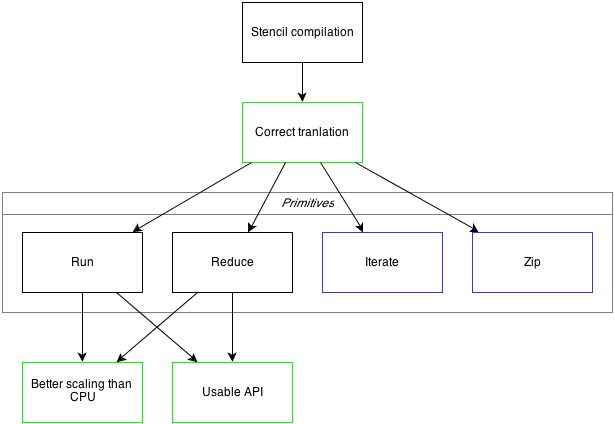
\includegraphics[width=\textwidth ]{figs/ypnos-task-dependency.pdf}
  \caption{This figure depicts the major task dependencies. The black boxes
    represent functional requirements, whereas the green boxes depict
    non-functional ones. Blue boxes are extensions.}
  \label{fig:task-dep}
\end{figure}

\section{Choice of Tools}

In this project I made use of both development tools, such as programming
languages and source control, as well as libraries for software reuse. Below, I
discuss the advantages and disadvantages of the tools, languages, and libraries
chosen

To familiarise myself with Ypnos, Accelerate and other tools, I started with
implementing sample functions in both. The main sample function was an average
stencil (which calculates the mean of its neighbour cell). Example code for this
stencil was given in \autoref{lst:ypsyn1} and will be discussed in detail in
\autoref{sec:introduction-ypnos}.

\subsection{Programming Languages}

Haskell was the obvious choice of programming language, given that Ypnos is
already developed in it. Having not programmed in Haskell before, I had to
become familiar with its more advanced features which were required by my
project (see \autoref{chap:impl}): \emph{type classes}, \emph{type families} and
\emph{data families}.

Haskell has excellent tools for developing compilers: strong typing, pattern
matching and mature parsing libraries
(Parsec\footnote{\url{http://hackage.haskell.org/package/parsec}}).
Furthermore, using the same language as the original implementation allowed for
much code reuse.

\subsection{Development Tools}

To aid the fetching of dependencies and the building of various targets I used
the \emph{Cabal} build system for
Haskell\footnote{\url{http://www.haskell.org/cabal/}}. Cabal features automatic
dependencies resolution and fetching as well as project building tools. By
writing some toy functions to test my knowledge of the Ypnos language I was also
able to set up a test build system in Cabal that I would later use in the rest
of my project. Cabal was chosen as it allowed me to automatically fetch and
install all the dependencies for my project as well as manage their versions and
compatibility.

\emph{Git} version control was used extensively throughout this project for
logging and backup. Although I was already quite familiar with this system, the
project allowed me to make use of some of Git's more advanced features such as
\emph{stashing}, \emph{sub-projects} and \emph{branching}. It was chosen
primarily for these advanced features as well as tight integration with free
hosting services such as \emph{Github}. This allowed my project to be frequently
backed up to the cloud.

\subsection{Libraries}
\subsubsection{Accelerate}

\emph{Accelerate} is a Haskell library which provides GPU accelerated array
computations. It is the only GPU programming library in Haskell which is
sufficiently powerful for my needs.

I chose Accelerate because of the native Haskell support and stencil
operations. It allowed me to abstract away from compiling to low-level C code
and, instead, concentrate on translating to a more abstract and general API.

Accelerate is discussed further in \autoref{sec:intr-axle}.

\subsubsection{CUDA}

\emph{CUDA} is a General Purpose GPU platform for NVidia devices\cite{cuda}. It
is the oldest framework of its kind but has recently been joined by the more
cross-platform OpenCL. The reason I chose CUDA over OpenCL was that the library
support in Haskell had the most stable support for it (though some experimental
support for OpenCL also exists).

As I do not own a machine with a CUDA enabled graphics card, I was using a
remote machine located in the Computer Laboratory. The sample functions allowed
me to set up the machine with the drivers and configuration required in order to
run the Accelerate library.

\section{Software Engineering Techniques}

This section highlights the software engineering approach taken in the
development of this project.

\subsection{Iterative Development}
\label{sec:iterdev}

Given my unfamiliarity with Haskell and GPU programming I followed the
\emph{iterative} model~\cite{cockburn08} to integrate exploration with
development. The end goal is to satisfy the project requirements. This and the
time constraints are the limiting factors of the iterative cycle.

\begin{figure}
  \centering
  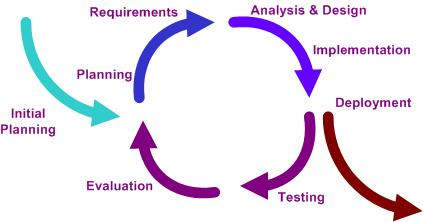
\includegraphics{./figs/Iterative_development_model_V2.jpg}
  \caption{One possible iterative development cycle. In the case of my project
    the deployment stage happened at the deadline and did not include a roll-out
    to actual customers. \\ \emph{Image courtesy of Wikipedia}}
  \label{fig:iterative}
\end{figure}

An iteratively developed project starts with an inception phase in which initial
requirements and goals are layed out. The project then proceeds through cycles
which consist of the following stages (see \autoref{fig:iterative}):

\begin{itemize}
\item
  Gathering requirements
\item
  Design
\item
  Coding
\item
  Testing
\item
  Evaluation
\end{itemize}

The first and last stages in the cycle merge together as requirements for the
next iteration feed off the examination of the last. After each cycle there is
an optional deployment phase in which the product is released. This phase is
omitted from the project.

Throughout the project various solution were attempted in phases and
re-evaluated based on issues found in the last iteration.  Iteration finished
when the requirements were met and the time limit reach.

\subsection{Test-Driven Development}
\label{sec:tdd}

The correctness of my implementation was a central goal. In order to achieve
this I took a test-driven approach to development: while writing the
implementation I was simultaneously writing unit tests for the code.  The
approach allowed me to quickly and effectively find bugs which had not already
been found by the Haskell type system.

\emph{QuickCheck} is the Haskell unit testing library\cite{claessen2011} used
throughout this project. QuickCheck and the testing methodology are discussed in
more detail in \autoref{sec:correctness}.

\section{Introduction to Ypnos}
\label{sec:introduction-ypnos}

Ypnos is an existing language with a fully formed syntax and a partial reference
implementation. Before I could start coding the translation from Ypnos to GPU, I
first had to understand and appreciate the reasoning behind the current choices
in the language and implementation.
\begin{figure}[!h]
\centering
% Define block styles
\tikzstyle{block} = [rectangle, draw,
    text width=6em, text centered, minimum height=4em]
\tikzstyle{ypnos} = [block, fill=blue!20]
\tikzstyle{haskell} = [block, fill=yellow!20]
\tikzstyle{bin} = [block, fill=gray!30]
\tikzstyle{surround} = [block, fill=gray!20]
\tikzstyle{line} = [draw, -latex']

\begin{tikzpicture}[row sep=0.5em]
  % Place nodes
  \def\x{7em}
  \node (9) {};
  \matrix[right=of 9] (1)
  {
    \node (title1) {Phase 1};\\
    \node [ypnos] (ypnos1) {Ypnos syntax}; \\
    \node [haskell] (haskell1) {Haskell code}; \\
    \node [ypnos] (libs) {Ypnos primitives}; \\
  };
  \matrix[right=\x of 1] (2)
  {
    \node (title2) {Phase 2}; \\
    \node [haskell] (haskell2) {Haskell code}; & \\
    \node [ypnos] (libs2) {Ypnos primitives}; & \\
  };
  \matrix[right=\x of 2] (3)
  {
    \node (title3) {Phase 3}; \\
    \node [bin] (bin) {Binary};\\
  };
  \begin{pgfonlayer}{background}
    \node [surround] (hasprim1) [fit = (haskell1) (libs)] {};
    \node [surround] (hasprim2) [fit = (haskell2) (libs2)] {};
    \node [surround] (background1) [fit = (title1) (hasprim1)] {};
    \node [surround] (background2) [fit = (title2) (hasprim2)] {};
    \node [surround] (background3) [fit = (title3) (bin)] {};
    \node [haskell] (hasprim1) [fit = (haskell1) (libs)] {};
    \node [haskell] (hasprim2) [fit = (haskell2) (libs2)] {};
  \end{pgfonlayer}
  % Draw edges
  \path [line] (background1) --
  node [midway, text width=6em, text centered, below] {Compile-time macros}
  (background2);
  \path [line] (background2) --
  node  [midway, below] {Compile} (background3);
\end{tikzpicture}
\caption{The compilation stages of an Ypnos program.\label{fig:comp-stages}}
\end{figure}

Ypnos consists of a library with various primitives used as the building blocks
of programs. Ypnos also provides some custom syntax via macros (see
\autoref{fig:comp-stages}).

\subsection{Grids}

The core data type in Ypnos is the \emph{grid}. As previously mentioned in
\autoref{sec:ypnos}, the grid is Ypnos' generalisation of the array. Unlike
the array, an Ypnos grid is implementation agnostic and could be implemented
differently with different backends.

Ypnos is designed with higher dimensions in mind so the grid may be
multi-dimensional (1D, 2D, etc.). In theory, the variable dimensionality of the
grids allows Ypnos stencil operations to be n-dimensional (although the
implementation doesn't currently support this).

\subsection{Parallelisation}

The stencil as a pattern is particularly good at exposing SIMD parallelism. On
systems like GPUs the amount of data sharing allowed is
restricted\footnote{Access to global shared memory (between thread blocks) is
  expensive. Instead thread block local memory should be used.}, which means
that operations on the different cores must be highly data parallel.

By \emph{subdivision} we are able to split a large grid into many subgrids (see
\autoref{fig:sten-decomp}). The stencils can operate over their subgrids in
parallel because the write-back points of each stencil never overlap. Therefore,
the stencils can safely read from a shared source grid.

\begin{figure}[h]
\centering
\begin{subfigure}{0.45\textwidth}
\centering
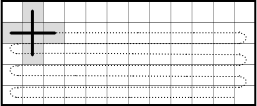
\includegraphics[width=0.95\textwidth]{figs/stencil-diagram.pdf}
\caption{Before subdivision}
\end{subfigure}
~
\begin{subfigure}{0.45\textwidth}
\centering
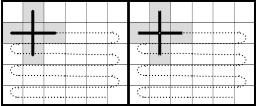
\includegraphics[width=0.95\textwidth]{figs/stencil-parallelised.pdf}
\caption{After subdivision}
\end{subfigure}
\caption{Subdivision of a grid for a 5-point stencil. The cursor location is
  shifted across the whole grid to produce a new grid.}
\label{fig:sten-decomp}
\end{figure}

\subsection{Stencil Syntax}

The Ypnos language provides a custom syntax for defining stencil functions as
well as a collection of primitive operations for their manipulation and use.

The code for a simple two dimensional averaging stencil is shown in
\autoref{lst:ypsyn2}.

\begin{hlisting}[label={lst:ypsyn2},caption={The simple mean function from \autoref{lst:ypsyn1}}]
avg2D :: Grid (Dim X :* Dim Y) a -> a
avg2D = [fun| X*Y:|_  a _|
                  |b @c d|
                  |_  e _| -> (a + b + c + d + e )/5|]
out = run avg2D in -- Running the stencil on `in' to produce `out'
\end{hlisting}

Compare this with the much more verbose imperative version of the same stencil
in \autoref{lst:avgimp}.  The \texttt{fun} macro is used to provide a
special \emph{grid pattern} syntax. The basic syntax of Ypnos can be summarised
as follows:

\begin{tabular}{p{0.1\textwidth} p{0.8\textwidth}}

  \texttt{X*Y:} & The syntax defines the dimensionality of the
  stencil. \texttt{X} and \texttt{Y} are both dimension variables (as is
  \texttt{Z}). They are combined usingthe \texttt{*} operator.  \\

\texttt{|} & The arguments are enclosed within pipe characters.  Their
arrangement in code is typically indented to reflect their grid shape.  \\

\texttt{a,b,\_} & Arguments can either be named or wildcard denoted
respectively with either a variable name or an underscore.  \\

\texttt{@} & This annotation denotes the variable is the cursor, the central cell whose position is used for the
result of the stencil (see \autoref{sec:primitives}).  \\

\texttt{->} & Delimiter that separates the grid pattern and the stencil body. It
appears to be normal Haskell syntax apart from recursion and function
definition.
\\

\end{tabular}

A generic stencil has a type of \texttt{Grid D a -> a} where \texttt{D} is the
dimensionality and \texttt{a} -- the element type. The dimensionality would take
the form \texttt{Dim X :* Dim Y} for a 2D grid.

\begin{hflisting}[label=lst:avgimp, caption={An imperative implementation of the
    average function. Note that the \texttt{in} index values have been laid out in the shape of the grid.}]
double in [M][N]; // Input array
double out [M][N]; // Output array
for (i = 1; i < M-1; i++){
  for (j = 1; j < N-1; j++){
    out[i][j] =
                 (in[i-1][j] +
     in[i][j-1] + in[i][j] + in[i][j+1]
                + in[i+1][j]) / 5;
  }
}
\end{hflisting}

\subsection{Primitives}
\label{sec:primitives}

As well as the syntax for stencil functions, Ypnos provides a library of
primitive operations. The primitives can be combined to create complex
accelerated computations over grids. The main primitive in Ypnos is \emph{run}
(see \autoref{lst:run-red}), which applies the stencil computation to a
grid.

\begin{hflisting}[label={lst:run-red}, caption={The basic \texttt{run},
\texttt{reduce} and, \texttt{reduceR} primitive as defined in the original Ypnos
paper\cite{ypnos-damp10}. \texttt{reduceR} provides a more general version of
the reducer allowing for intermediary values.}]

run :: (Grid D a -> b) -> Grid D a -> Grid D b

reduce :: (a -> a -> a) -> Grid D a -> a

reduceR :: Reducer a b -> Grid D a -> a
mkReducer :: exists b. (a -> b -> b)
                    -> (b -> b -> b)
                    ->  b
                    -> (b -> c)
                    -> Reducer a
\end{hflisting}

The application is done by moving the stencil cursor over each location in the
grid (we saw this illustrated in \autoref{fig:sten-decomp}). The arguments of
the stencil are taken from positions in the grid relative to the cursor. The
value is then computed using the specified computation and put into the same
cursor location in a \emph{new} grid.

In some locations near the edge of the grid there may not be enough neighbours
to satisfy a stencil. In this case Ypnos provides a special syntax for dealing
with these \emph{boundaries}. The implementation of boundaries is beyond the
scope of this project. However, a brief description of their behaviour will aid
the reader's understanding.

For each boundary of the grid, outside of which the stencil may access, a value
is computed by a user defined function. The function may use the current
location index and values from the grid (accessed via a specially bound
variable). A common boundary -- the \emph{mirror} boundary -- works by providing
the closest value inside the grid when an outside access is made. This is the
boundary that I have tacitly assumed to be default in my implementation.

Another vital primitive of the Ypnos language is the \emph{reduce} primitive
whose purpose is to summarise the contents of a grid in one value (see
\autoref{lst:run-red}). It may be used to compute functions such as the mean,
sum or minimum/maximum.

The primitive uses an associative operator (of type \texttt{a -> a -> a}) to
combine all the elements of the grid to one value. A more general version of
this operator, \emph{reduceR}, also exists (see \autoref{lst:run-red}),
which supports an intermediary type (or partial value).

The \emph{Reducer} data type takes the following parameters:

\begin{itemize}
\itemsep1pt\parskip0pt\parsep0pt
\item
  a function reducing an element and a partial value to a partial value,
\item
  a function reducing two partial values,
\item
  a default partial value
\item
  and a conversion from a partial value to the final value.
\end{itemize}

This Reducer is passed into the \emph{reduceR} primitive taking the place of the
associative operator in the reduce primitive. Clearly, reduce can be implemented
in terms of reduceR and so the latter is the more general.

\section{Introduction to Accelerate}
\label{sec:intr-axle}

We have already mentioned Accelerate as one of the implementors of stencil
convolution. In fact, Accelerate is an excellent target for intermediary code
compilation. While the stencil semantics of Accelerate and Ypnos differ in some
respects, the former is powerful enough to represent the latter. Therefore, the
project will target the Accelerate language instead of CUDA.

Accelerate uses the Haskell type system to differentiate between arrays
on the CPU and GPU. It does this by introducing a type encapsulating GPU
operations. There is a further \emph{stratification} of this type into
scalar and array values. Scalar computations may be composed into
array computations.

\subsection{GPU Computation}

For a process on the CPU to execute a CUDA program it must first send
the program and the data to the GPU. When the result is ready it must be copied
back into the main memory of the process concerned. I will call these two
procedure \emph{copy-on} and \emph{copy-off} respectively (see
\autoref{fig:copyonoff}).

\begin{figure}[tb]
  \includegraphics[width=\textwidth]{figs/copyonoff.pdf}
  \caption{An illustration of copy-on and copy-off times.  }
  \label{fig:copyonoff}
\end{figure}

Accelerate represents this difference in the type system. The \texttt{Acc} type
denotes an operation on the GPU. For the purposes of Accelerate, the only
operations allowed on the GPU are those over arrays. As such, \texttt{Array sh
  e} denotes an array of shape \texttt{sh} and element type \texttt{e}.
\texttt{Acc (Array sh e)} denotes the same but in GPU memory and encapsulate an
operation. This means that when such an array is evaluated a CUDA program must
be executed on the GPU.

Arrays are signalled for use on the GPU via the \texttt{use} primitive.  They
are copied-on, executed and copied-off via \texttt{run}. This primitive is
responsible for the run-time compilation and actual data transfer. All other
operations build an abstract syntax tree (AST) to be compiled by the
\texttt{run} primitive. Together \texttt{use} and \texttt{run} form the
constructors and destructors of the \texttt{Acc} data type (see
\autoref{lst:runuse}).

\begin{hflisting}[label={lst:runuse}, caption=The basic constructors and
  destructors for moving arrays too and from the GPU in Accelerate.]
use :: Array sh e -> Acc (Array sh e)
run :: Acc (Array sh e) -> Array sh e
\end{hflisting}

\subsection{Stratified Language}

The main form of operation in Accelerate is over arrays. However, it is often
desirable to build arrays out of multiple scalar values or functions over
scalars. A classic example of this is the map function which transforms an
entire array by a function over the individual values\footnote{In fact, the map
  function is conceptually similar to stencil application. The difference being
  that stencils take into account the neighbourhood of a cell to compute
  the next value whereas map takes only the central value.}(\autoref{lst:map}). For this reason, in addition to the \texttt{Acc} type,
Accelerate also provides the \texttt{Exp} type where the former represents
collective operations and the latter represents scalar computations. The two
types correspond to the two different types of AST built: one for scalar and the
other for array operations.

\begin{hflisting}[label={lst:map}, caption=The type of the \texttt{map}
  operation as defined by Accelerate.]
map :: (Exp a -> Exp b) -> Acc (Array sh a) -> Acc (Array sh b)
\end{hflisting}

Scalar operations do not support any type of iteration or recursion in order to
prevent divergent operation at run-time. However, most other Haskell code is
allowed. This is achieved by the Haskell type class mechanism (for ad-hoc
polymorphism, discussed further in \autoref{sec:typeclasses})-- Accelerate
provides instances of \texttt{Exp a} for most common classes.

For example, to support addition, subtraction and other numerical operations,
Accelerate provides an instance of the type class \texttt{Num}. This means that
operations can be typed as shown in \autoref{lst:num}.

\begin{hlisting}[label={lst:num}, caption=The type of addition overloaded by Accelerate.]
(+) :: Exp a -> Exp a -> Exp a
1 + 2 + 3 :: Exp Integer
\end{hlisting}

\subsection{Stencil Support}

Whilst \texttt{map} for an array applies a scalar function to every element in
an array, Accelerate provides support for running stencil computations via the
\texttt{stencil} function (see \autoref{lst:sten}).

\begin{hflisting}[label={lst:sten}, caption={The type of the stencil application
  function in Accelerate. Including an example instance of the
  \texttt{Stencil} type class. Many others are also possible.}]
stencil :: Stencil sh a sten =>
           (sten -> Exp b) ->
           Boundary a ->
           Acc (Array sh a) ->
           Acc (Array sh b)

instance Stencil DIM2 a ((Exp a, Exp a, Exp a)
                        ,(Exp a, Exp a, Exp a)
                        ,(Exp a, Exp a, Exp a))
\end{hflisting}

The first parameter is a function which represents the stencil. We see that
\texttt{sten}, the type of the stencil argument, takes the form of a tuple grid
of \texttt{Exp a} element type. This allows Accelerate to use Haskell's function
syntax to define stencils.

The second parameter is the type of boundary. In Accelerate, the types of
boundary allowed are fixed as opposed to Ypnos boundaries which can be fully
specified. One of the types allowed is \texttt{Mirror} (see
\autoref{sec:primitives}).

With these two parameters we have defined an operation which performs the
stencil convolution. An example stencil function is given in
\autoref{lst:ypsten}.

\begin{hlisting}[label={lst:ypsten}, caption={The ``average'' stencil defined
  using Accelerate's syntax.}]
avg :: Exp a => Stencil3x3 a -> Exp a
avg (( _, a, _ )
    ,( b, c, d )
    ,( _, e, _ )) = (a + b + c + d + e) / 5

type Stencil3x3 = ((Exp a, Exp a, Exp a)
                  ,(Exp a, Exp a, Exp a)
                  ,(Exp a, Exp a, Exp a))
\end{hlisting}

\section{Summary}

In this section we have seen an analysis of the project's requirements which
allowed me to prioritise the work for the project. Based on the requirements a
choice of tools and libraries was made. An iterative approach to development was
chosen to meet as many of the requirements as possible in the time given.

At the beginning of the project, time was spent on familiarisation with the
tools and libraries as well as the Ypnos language itself. Complex parts of the
Haskell language were investigated and understood (type classes and
families). The Accelerate library, central to the project, was investigated and
``toy'' programs were implemented in both Ypnos and Accelerate.

\chapter{Implementation}
\label{chap:impl}

The work of the implementation can be roughly split into two large chunks: the
compilation of stencils and the implementation of the primitives. In this
project I am aiming for both an accurate and fast translation as well as one
which is easy for the programmer to use.

In this chapter I will highlight the major implementation approaches taken for
the stencil compilation and primitives as well as an example usage of the
system.

\section{Iterative Development}

The iterative development approach was followed throughout the implementation of
this project. \autoref{tbl:iter} describes the phases of development: each
phase consisted of a working code prototype and a small usability evaluation. In
the following sections I will describe each approach taken in more detail.

\begin{table}
\begin{tabular}{l l | p{11cm}}
  \hline
  Phase 1 & Motivation & Create a working translation and run primitive using Accelerate.\\
  & Produced & The non-unifying approach to primitives and compile time approach to stencil translation with centring (\autoref{sec:non-unify-appr} and \autoref{sec:typesysapp}).
  \\
  Phase 2 & Motivation & Reduce the code changes the programmer must perform and unify the CPU and GPU run primitives.\\
  & Produced & The run and reduce primitives using type class parameters (\autoref{lst:redgrid})
  \\
  Phase 3 & Motivation & Make the return type of the reducer more useful to the user.\\
  & Produced & The run and reduce primitives using data families (\autoref{lst:rundatafam}).
  \\
  Phase 4 & Motivation & Remove the need for the programmer to change many constructors when switching.\\
  & Produced & The final approach using a combination of type synonym families and type class parameters (\autoref{sec:final}).\\
  \hline
\end{tabular}
\caption{The phase of iterative development in this project: for each cycle the motivation and work produced is described. \label{tbl:iter}}
\end{table}

\section{Stencil Compilation}

Compilation of stencils was a central task in this project. The abstract Ypnos
syntax is compiled down to Haskell AST to be run. Accelerate's implementation
has overridden much of the Haskell operators required for this translation
stage, so the bulk of the effort went into producing the functions that contain
the stencil computations. These functions take the form of
\autoref{lst:ypsten}

The arguments are formed as tuples of tuples. The rest of the stencil is normal
Haskell code. However, the return type, \texttt{Exp a}, ensures that all the
operations actually use Accelerate's overridden methods to build an AST. The AST
is then translated at run-time into CUDA code.

Ypnos achieves its custom syntax via Haskell's quasiquoting mechanism, a
language feature which allows the library author to provide custom syntax for
domain specific languages\cite{mainland2007}. The programmer must provide a
parser object (refered to as a quasiquoter). The essential function of a
quasiquoter is to provide an abbreviation for entering the AST manually.

Take, for example, the situation in which we want to write an embedded
language to act as a calculator. We have the AST for our
simple calculator in \autoref{lst:calc}.

\begin{hlisting}[label={lst:calc}, caption={A simple calculator defined using an
  AST (\texttt{Expr}) and using a quasiquoter for abbreviated syntax. The definition of
  \texttt{expr} is omitted.}]
data Expr  =  IntExpr Integer
           |  BinopExpr (Integer -> Integer -> Integer) Expr Expr

e1 = BinopExpr (+) (IntExpr 1) (IntExpr 3)
e2 = [expr| 1 + 3 |]
\end{hlisting}

We see that the quasiquoter \texttt{expr} allows us to abbreviate the expression
\texttt{e1} to the more obvious form of \texttt{e2}.

We could sensibly do the translation from Ypnos to Accelerate stencils in one of
two ways: we (a) use Haskell's type system to mask the difference between the
two operations at compile-time or (b) we use run-time compilation to mask the
difference between the implementations. Benefits and drawbacks of both are
presented in the next section.

\subsection{Centring}
\label{sec:centring}

One way in which Accelerate and Ypnos stencils differ is that the former assumes
that the cursor is at the centre of an odd sized grid ($3 \times 5, 5 \times 5$)
whereas the later allows the user to specify the centre. Ypnos stencils can be
translated to Accelerate stencils by padding the stencil passed to Accelerate
such that the cursor is centred.

Take an example: assume a one dimensional stencil with the cursor at an
off-centre location (denoted by \texttt{c}) -- \autoref{fig:cursor}.

\begin{figure}
  \centering
  \begin{subfigure}[t]{0.45\textwidth}
    \includegraphics[width=\textwidth]{figs/align1.pdf}
    \caption{The stencil before centring. Note the even shape ($4\times1$).}
    \label{fig:cursor}
  \end{subfigure}
  ~
  \begin{subfigure}[t]{0.45\textwidth}
    \includegraphics[width=\textwidth]{figs/align2.pdf}
    \caption{The same stencil after centring. Note the shape is now odd
      ($5\times1$)}
    \label{fig:centredcursor}
  \end{subfigure}
  \caption{Where $a$ is the position of the cursor and $b$ -- the length of the
    stencil.  In this diagram $pad_{start}$ represents the offset which needs to
    be applied to the centre, i.e the amount to pad the start of the
    grid. $pad_{end}$ represents the amount to pad the end of the grid. }
\end{figure}

Now we must determine the padding such that the cursor is centred. This is given
by the following two equations:

\[ pad_{start} = max \{a, b-a-1\} - a \]

\[ pad_{end} = max \{a, b-a-1\} - (b - a - 1) \]

This means that after centring we get \autoref{fig:centredcursor}

In order to implement the centring I had to consider both the one and two
dimensional cases.  It would be quite easy to deal with this in two separate
cases, except it must be possible to extend the approach to higher dimensions. I
considered three principle approaches to doing this: using lists as
intermediaries; using arrays as intermediaries; or operating on the grid
patterns directly via type classes.  Before addressing the approaches I will
mention the types in question (see \autoref{lst:gridpattern}).

\begin{hlisting}[label={lst:gridpattern}, caption=The data type which stores
  the grid patterns in Ypnos. Notice that the dimensionality is not exposed in
  the type but hidden.]
data GridPattern = GridPattern1D DimTag [VarP] |
                   GridPattern2D DimTag DimTag [[VarP]]
\end{hlisting}

\texttt{GridPattern} is the type in the Ypnos AST corresponding to the parsed
pattern of arguments. We see that it takes both a 1D and 2D form where the
variables (their type is \texttt{VarP}) are a list and a list of lists
respectively. We may also note that the dimensionality is expressed directly in
the constructor and as such is not present in the type.

The pattern of arguments in Accelerate is expressed as a tuple in the 1D case
and a tuple of tuples in the 2D case. This representation contains no explicit
information about which variables are cursors as we discussed in the previous
section.

\subsubsection{Type Classes}
\label{sec:typeclasses}

Haskell provides both \emph{parametric} and \emph{ad-hoc} polymorphism. The
former is provided by default in function definitions: each function is made to
work over the most general type possible. The latter is provided via the
mechanism of \emph{type classes}.  I required ad-hoc polymorphism in order to
operate differently on patterns of different dimensionalities.

A type class is declared in two parts: interface and instance. An interface has
a number of type parameters (also called indices) and function type
declarations. It is then possible to declare which types are instances of which
class. This is done by providing concrete types for the indices and concrete
definitions for the functions. \autoref{lst:typeclass} gives an example of a
type class declaration and instance.

\begin{hlisting}[label=lst:typeclass, caption={An example type class for
    equality. Showing the declaration and the instance for integers. Where
    \texttt{integerEq} is the implementation of integer equality on the target
    machine.}]
class Eq a where
  (==) :: a -> a -> Bool

instance Eq Integer where
  x == y =  x `integerEq` y

\end{hlisting}

\subsubsection{Type Families}
\label{sec:typefam}

Type families (also known as indexed type families) allow us to apply the same
kind of parameterisation as in type class to the
types\cite{chakravarty05}. Formally, type families are type functions from one
or more types to a single type. As with type classes there are both head
declarations and instances which define the family. The declaration describes
the \emph{``kind''}\footnote{A kind is the type theoretic name for a type for
  types. \texttt{*} denotes the kind of base types in Haskell.} of the family
and defines how many type arguments are taken.

Type families come in two flavours: data families and type synonym families. The
former allows the data type to be declared differently for different indexes,
whereas the latter allows different types to be synonymous.
\autoref{lst:datafam} gives an example of a data family being used to expose
the dimensionality of a pattern. This allows for the use of ad-hoc polymorphism
later on.

\begin{hlisting}[label=lst:datafam, caption=The data family declares tw<
  different constructors for 1D and 2D lists. The dimensionality of the list is
  exposed in the type.]
data family GridPatt :: * -> * -> *
data instance GridPatt (Int) a     = GridPatt1D Int [a]
data instance GridPatt (Int,Int) a = GridPatt2D (Int, Int) [[a]]
\end{hlisting}

Both flavours can be associated with a type class. In this case the index of the
type class must form part of the index of the type family. The interface and
instance declarations of the type family are bound to the corresponding
declarations of the type class. \autoref{lst:assoctypefam} gives an example
of an associated data family for patterns as opposed to it standing alone in
\autoref{lst:datafam}. The usage of type synonym families will be discussed
in detail in \autoref{sec:intr-type-class}.

\begin{hlisting}[label=lst:assoctypefam, caption={The data family from
    \autoref{lst:datafam} has now been associated with the class
    \texttt{GridIx} to provide the function \texttt{size} for various
    dimensionalities.}]
class (Ix i, Num i, ElMax i) => GridIx i where
    data GridPatt :: * -> * -> *
    size :: GridPatt i a -> i

instance GridIx (Int) where
    data GridPatt (Int) a = GridPatt1D Int [a]
    size (GridPatt1D s _) = s
\end{hlisting}

\subsubsection{Intermediate Approaches}

The first approach to centring taken involved first converting from grid
patterns into lists, then balancing these lists, and finally converting them
into the centred tuples needed for the Accelerate functional representation. In
order to do this I would have to define functions for measuring the location of
the cursor, and padding the lists before and after. This approach proved
difficult as lists did not explicitly incorporate their dimensionality in the
type. This made it hard to treat the 1D and 2D cases differently.

The second approach attempted to use existing array code in order to avoid
writing such functions. The hope was that by converting to arrays, rather than
lists, functions for appending and prepending rows and columns would already
exist. However, this was not the case and I would have had to write these
myself. As such, the intermediary array stage was not the best choice.

\subsubsection{Direct Approach}

The third and final approach was to operate directly on the lists extracted from
the \texttt{GridPattern} types. As previously mentioned, to retain
dimensionality information in the type system a type class was required.  I
designed a class \texttt{GridIx} (see \autoref{lst:gridix}) to perform the
basic operations -- \texttt{addBefore}, \texttt{addAfter}, \texttt{find} and
\texttt{size} -- in a dimension-sensitive way while still being polymorphic.

\begin{hlisting}[label={lst:gridix}, caption=The class declaration of
  \texttt{GridIx} showing the main functions defined for the grid manipulation
  and an associated data family.]
class (Ix i, Num i, ElMax i) => GridIx i where
    data GridPatt i :: * -> *
    addBefore :: i -> a -> GridPatt i a -> GridPatt i a
    addAfter :: i -> a -> GridPatt i a -> GridPatt i a
    find :: (a -> Bool) -> GridPatt i a -> i
    size :: GridPatt i a -> i
\end{hlisting}

The associated data type \texttt{GridPatt} would take the type of the particular
dimensionality of list that is appropriate for a given instance. In the case of
the index type \texttt{Int} we would get \texttt{GridPatt Int a = {[}a{]}} and
in the case of \texttt{(Int, Int)} we get \texttt{{[}{[}a{]}{]}}. This approach
allows the algorithms for centring to be described more generally regardless of
the number of dimensions actually involved.

This is the best and most efficient approach in terms of code reuse. This is why
I adopted this approach in the centring used for compile-time stencil
translation (described next).

\subsection{Compile-time Approach to Translation}
\label{sec:typesysapp}

As we saw in the previous section, the types of the Ypnos CPU stencil and the
Accelerate library's stencil differ wildly. \autoref{lst:avgsten} shows the
difference for the \texttt{avg}\footnote{For the sake of simplicity I have
  excluded the type constraints relating to boundaries as these are long
  and complicated.}  stencil.

\begin{hlisting}[label={lst:avgsten}, caption={The average function implemented
    on both the CPU and GPU. Note the difference in types. The constraints are
    simplified.}]
avgCPU :: (Array a, Floating a) => Grid (Dim X :* Dim Y) a ->     a
avgGPU ::      Floating (Exp a) =>            Stencil3x3 a -> Exp a
\end{hlisting}

In the GPU case we see that the type (once expanded) is tuples of tuples of
\texttt{Exp a}. On the other hand, in the Ypnos case we see that arguments take
the form of a grid, which is exactly the same type as the grids it operates on.

The Ypnos grid type is a \emph{comonad}, a functional programming design pattern
arising from Category Theory. The run primitive is an operation of the comonad,
\texttt{cobind} (\autoref{lst:cobind}).

\begin{hflisting}[label={lst:cobind}, caption={The definition of cobind. Let
    \texttt{D} be a grid of a certain dimension and \texttt{a} and \texttt{b} be
    the types of that grid.}]
cobind :: (D a -> b) -> D a -> D b
\end{hflisting}

The type system approach (or compile-time approach) means that Ypnos stencil
syntax is translated directly to a function with Accelerate type
(e.g. \texttt{avgGPU}) by using a different quasiquoter. This was implemented by
me in the \texttt{funGPU} quasiquoter (see \autoref{sec:usage} for usage
examples). Advanced type-system features in Haskell are used to unify the two
types of stencils. The pros and cons of this approach will be discussed in
\autoref{sec:prims}.

Unfortunately, by translating directly to the Accelerate stencil type we lose
the comonadic nature of the type. This is a shame, because this type is both
informative to the programmer (as it is a functional pattern), yet flexible
enough that by changing the instance of \texttt{D} we change the implementation.

The advantage of this method is that all the translation effort is done at
compile-time allowing the running of the stencil to be more efficient.

\subsection{Run-time Approach to Translation}
\label{sec:runtimetrans}

The second approach to the translation of stencils was to keep the types the
same as Ypnos' original implementation.  This is alluring as it allows us to
both expose more information to the user through the program's type and maintain
the theoretic underpinnings of Ypnos -- the comonadic structure. In order to
achieve this, some run-time conversions had to be done.

As already seen, we would like the \texttt{run} primitive to take the
form given in \autoref{lst:run2}

\begin{hflisting}[label={lst:run2}, caption=The comonadic run type. Changing the
  type of \texttt{g} could change the backend used.]
run :: Comonad g => (g a -> b) -> g a -> g b
\end{hflisting}

We have also seen that Accelerate does not accept stencils of this type (see
\autoref{sec:typesysapp}).  To solve this we previously broke the
comonadicity of the operation but we could attempt to preserve it by introducing
an \emph{arrow} data constructor to abstract the differences in type between the
notion of a stencil function\ in Accelerate and Ypnos. This changes the run
function to that seen in \autoref{lst:runarr}.

\begin{hlisting}[label={lst:runarr}, caption=The type run is generalised to
  using the \texttt{arrow} type.]
run :: Comonad g => (g a `arrow` b) -> g a -> g b
\end{hlisting}

The \texttt{arrow} constructor is parametrized on both \texttt{g a} and
\texttt{b}. To build up an instance of \texttt{arrow} we must pass in the
stencil function to a special constructor. The constructor chosen decides the
implementation used.

While previously (\autoref{sec:typesysapp}) we had to use different versions
of the quasiquoter to produce different stencils at compile-time, we now use the
same quasiquoter but convert the function at run-time. We achieve this by taking
advantage of Haskell's polymorphism which allows a function over type \texttt{a}
to specialise to a function of type \texttt{Exp a'}. This generalisation
combined with the arrow data constructor allows our stencil functions to have
the type in \autoref{lst:arrow-sten}

\begin{hlisting}[label={lst:arrow-sten}, caption=Here we see the type the
  stencil must have in Accelerate (\texttt{stencil}) and the type we can
  generalise to using the \texttt{arrow} type (\texttt{stencil'}).]
stencil :: Comonad g => g (Exp a) -> Exp b
stencil' :: Comonad g => g a `arrow` b
\end{hlisting}

Because of the arrow type, \texttt{stencil} and \texttt{stencil'} can now have
the same type.

The type of stencil accepted by Accelerate is still not of the form \texttt{g
  (Exp a) -\textgreater{} Exp b}. A conversion function builds an Accelerate
stencil (call it \emph{stencil A}) at run-time using the stencil encapsulated in
the arrow data type (call it \emph{stencil B}). Stencil A's arguments are used
to build up a grid of type \texttt{g (Exp a)}, then stencil B is used on this
grid to produce the result of type \texttt{Exp b}, finally this is returned as
stencil A's result. So stencil A behaves as a wrapper around stencil B.

While this run-time conversion creates an overhead, it also simplifies the types
significantly. A technique called deforestation may be used to mitigate the
overhead\footnote{Deforestation is also known as ``short cut fusion''. It is
  essentially an optimisation which eliminates intermediate data
  structures.}. Such optimisation is beyond the scope of this project due to
time constraints.

\section{Primitives}
\label{sec:prims}

The primitives are the second core component of the port to GPU. The
implementation of the primitives had two potential approaches: the first was to
re-implement the primitives in a separate module (a non-unifying approach). In
this case, the user would import whichever implementation they required. This
approach had some drawbacks -- for example, it required the user to change much
of their code between implementations.

This led to the second approach of extracting the functionality of the primitive
into a type class. This solution required the use of some complicated type
features in order to make the types unify. This lead to a further three
possibilities: (a) using a type class parameter for unification, (b) associating
a type family and (c) associating a data type.

The resultant approach was a hybrid of these. In this section I will detail all
the approaches taken and at the end of this section I will discuss the
trade-offs which lead to the final approach.

\subsection{Non-unifying Approach}
\label{sec:non-unify-appr}

The run primitive implemented in Phase 1 (see \autoref{tbl:iter}) used the
compile-time implementation of the stencil function
(\autoref{sec:typesysapp}). At the highest level this meant that the function
\texttt{run} had type given in \autoref{lst:runtype}.

\begin{hlisting}[label={lst:runtype}, caption=The type of run required by Accelerate.]
run :: (Stencil sh x sten) => (sten -> Exp y) -> Grid d x -> Grid d y
\end{hlisting}

However, we see that the type variable \texttt{sh} (required by Accelerate) and
\texttt{d} (required by Ypnos) do not unify requiring another constraint to
reconcile the two. Furthermore, constraints need to then be added for the types
of \texttt{x} and \texttt{y} to satisfy Accelerates \texttt{stencil}
function. In the end this type becomes unwieldy -- it is not straight-forward
for the user to write in their code.

Similar problems would have plagued the implementation of the \texttt{reduce}
primitive. However, having first seen the implementation of the \texttt{run}
primitive I decided that a different approach was necessary so this incarnation
of the \texttt{reduce} primitive was never implemented.

\subsection{Introducing Type Classes}
\label{sec:intr-type-class}

In this project I am aiming to make both an accurate and fast translation as
well as one which is easy for the programmer to use.  With the previous approach
we saw how this did not work for two reasons: (a) the run primitive I
implemented was not related (as far as Haskell was concerned) to the original
CPU primitive, and (b) the types of the two primitives differed, which could
cause compilation to fail if they were swapped.

The ideal would be a function which behaves differently under certain program
conditions. The perfect tool for this job is ad-hoc polymorphism which is
provided in Haskell via type classes (see \autoref{lst:avgsten}). The result is
an implementation of the primitive which changes dependent on a particular type
parameter. The obvious parameter in our case is the grid type, that is, have
different grid types for different backends.

We have seen this before: in some of the code examples I have used the notation
``Comonad g'' to refer to a grid which implements the primitives of Ypnos. This
was a type class approach. However, we run into the same problems as with
stencil translation (see \autoref{sec:runtimetrans}), namely the types of
stencil required by Accelerate and Ypnos differ.

\subsubsection{Type Class Parameter}

\begin{hflisting}[label={lst:redgrid}, caption={The \texttt{ReduceGrid} type
class defined with type parameters for each variable: \texttt{a}, \texttt{b} and
\texttt{c}. The \texttt{RunGrid} type class has type parameter \texttt{grid} and
\texttt{sten} where the later is fully determined by the former.}]
class ReduceGrid grid a b c | grid -> a,
                              grid -> b,
                              grid -> c where
    reduceG :: Reducer a b c-> grid -> c

data Reducer a b c where
    Reducer ::   (a -> b -> b)
              -> (b -> b -> b)
              -> b
              -> (b -> c)
              -> Reducer a b c

instance ReduceGrid CPUGrid a b c where
    reduceG = undefined -- Not implemented
instance ReduceGrid GPUGrid (Exp a) (Exp b) (Exp c) where
    reduceG = undefined -- Not implemented

class RunGrid grid sten | grid -> sten where
    runG :: sten -> grid -> grid

instance RunGrid CPUGrid CPUStencil
instance RunGrid GPUGrid GPUStencil
\end{hflisting}

The approach taken in Phase 2 to reconciling the stencil uses Haskell type
classes parametrized by more than one type. This allows us to abstract over
parts of the type that change to give a unified type. As the reduce primitive
was the first to bring about such issues, let's examine how this approach can be
applied to it (see \autoref{lst:redgrid}).

In this approach we are able to have instances for \texttt{Reducer} for the CPU
and GPU based on the grid type yet we also change the types of values accepted
by the functions of the Reducer. These types correspond to different types of
functions (\texttt{Exp a}) which tells Haskell to use Accelerate's overloaded
versions of operators.

We also see that the \texttt{RunGrid} type class is treated in a similar manner:
the type of grid uniquely determines the type of stencil function required. This
is achieved in Haskell using a \emph{functional dependency} (\texttt{grid ->
  sten}) meaning that the \texttt{grid} parameter uniquely determines the
\texttt{sten} parameter\cite{jones2000}. We see this a couple of times in the
given example.

Unlike the \texttt{reduceG} example, Haskell cannot, without help from the
programmer, choose a different quasiquoter (as is required with the static
approach as seen in \autoref{sec:typesysapp}).

\needspace{3\baselineskip}
In theory, this approach should work, however, it brings some usability
problems. Let's further examine the type of the \texttt{reduceG} primitive
when applied to \texttt{GPUGrid}s (see \autoref{lst:redgpu})

\begin{hflisting}[label={lst:redgpu}, caption={The type of the reducer once the
    Accelerate types are applied.}]
Reducer :: (Exp a -> Exp b -> Exp b)
        -> (Exp b -> Exp b -> Exp b)
        -> (Exp b) -- Default value
        -> (Exp b -> Exp c)
        -> Reducer (Exp a) (Exp b) (Exp c)
reduceG :: Reducer (Exp a) (Exp b) (Exp c)
        -> GPUGrid
        -> Exp c -- Return value
\end{hflisting}

Notice that both the return value and default value of the reducer have type
\texttt{Exp}, which is problematic, as \emph{lifting} and
\emph{unlifting}\footnote{Lifting is the process of promoting something of type
  \texttt{a} to type \texttt{Exp a}. Unlifting is the inverse process. Both
  aren't always possible.}  is not easy for the user to do and the wrapped value
is not particularly useful or meaningful once returned to the user. One approach
to changing this would be to introduce type parameters for the functions rather
than the values. However, the approach taken next offers greater flexibility.

\subsubsection{Associated Type Families}
\label{sec:assoctypefam}

We already encountered associated type families in
\autoref{sec:typefam}. Here we will be using type synonym families as
opposed to data families (Phase 4). These allow the unification of the different
function types required (see \autoref{lst:typesynfam} for an example of type
synonyms families unifying different function types).

\begin{hflisting}[label=lst:typesynfam, caption=The type synonym family is used
  as a type function. It is used to work out the element type of a collection.
  Here the \texttt{Fun} family (representing a one-argument function) can take
  two forms depending on the compilation target.]

type family Fun :: * -> * -> * -> *
type instance Fun CPUGrid a b = (a -> b)
type instance Fun GPUGrid a b = (Exp a -> Exp b)

\end{hflisting}

\needspace{7\baselineskip}
The ideal type for the \texttt{Reducer} in the GPU implementation is given in
\autoref{lst:reduceideal}

\begin{hlisting}[label={lst:reduceideal}, caption={The optimal type for the
    reduce primitive under Accelerate.}]
Reducer :: (Exp a -> Exp b -> Exp b)
        -> (Exp b -> Exp b -> Exp b)
        -> b -- Unlifted default
        -> (Exp b -> Exp c)
        -> Reducer a b c

reduceG :: Reducer a b c -> GPUGrid -> c -- Unlifted return
\end{hlisting}

\needspace{14\baselineskip}

This make the default easier to provide and result easier to use. By examining
this we can deduce that there are actually two types of abstract function
involved: 1- and 2-argument functions of \texttt{Exp}s. If we implement these as
two associated type families we get the behaviour required (see
\autoref{lst:redtypefam})

\begin{hlisting}[label={lst:redtypefam}, caption={The application of type
    families to the reduce primitive.}]
Reducer :: Fun2 g a b b
        -> Fun2 g b b b
        -> b
        -> Fun1 g b c
        -> Reducer g a b c

class ReduceGrid g where
    type Fun1 g a b
    type Fun2 g a b c
    reduceG :: Reducer g a b c -> g -> c
\end{hlisting}

Next I wanted to extend this approach to the run primitive. However, with run we
do not simply have a conversion of types, but also conditions on those types
(called constraints in Haskell). It is possible to encode constraints in a type
family method using a Haskell language extension called
\emph{ConstraintKinds}. This allows us to define a type family which has the
\emph{kind} of \texttt{Constraint} instead of the usual \texttt{*} (denoting
type as seen in \autoref{sec:typefam}). An example of the \texttt{RunGrid}
class modified in this way is given in \autoref{lst:constkind}.

\begin{hlisting}[label={lst:constkind}, caption={The application of type
    families to the run primitive.}]
class RunGrid g where
    type ConStencil g a b sten :: Constraint
    type Stencil g a b sten :: *
    run :: ConStencil g a b => (Stencil g a b) -> g x -> g y

instance RunGrid g where
    type ConStencil g a b sten = (Stencil sh a ~ sten, ShapeOf g ~ sh)
    type Stencil g a b sten = sten -> Exp b
\end{hlisting}

As we see, using associated type families is not general because we are exposing
\texttt{sten} -- a type variable which has no relevance to the CPU
implementation. Though it can be safely ignored, it exposes too much of the
underlying type difference which we are coding against and so does not decouple
the two implementations. As we will see in \autoref{sec:final}, this problem
can be mitigated by taking a hybrid approach.

\subsubsection{Associated data families}
\label{sec:assoc-data-fam}

Associated type families make the type of the stencil function explicit again
(Phase 3), as with the type class parameter. To achieve this we can make use of
associated data families (see \autoref{sec:typefam}). These work in much the
same way as type families, but rather than binding a particular synonym to a
class we bind a data type definition.

\autoref{lst:rundatafam} shows the \texttt{RunGrid} type class defined using
data families. We can see that the data family has replaced both the type and
constraint families from \autoref{sec:assoctypefam}.

\begin{hflisting}[label=lst:rundatafam,
caption=RunGrid with associated data family.]
class RunGrid g where
    data Sten g a b :: *
    runG :: Sten g a b -> g a -> g b
\end{hflisting}

This is done with \emph{generalized algebraic data types} (GADTs, another
Haskell type extension) which, amongst other things, allow us to place arbitrary
type constraints on constructors (\autoref{lst:stendatafam}).

\begin{hlisting}[label=lst:stendatafam,
caption={An example of a stencil data type for the GPU. Note the argument it takes is a stencil function (of type \texttt{sten -> Exp b}) where \texttt{sten} has been constrained in the required way.}]
data Sten (Array sh) a b where
        Sten :: (Shape sh, Stencil sh a sten,  -- constraints
                 Elt a, Elt b) =>              -- |
                (sten -> Exp b)
                -> Sten (Array sh) a b
\end{hlisting}

This allows for much cleaner implementation on our part but requires the
programmer to use different data constructors for the different implementations
(CPU versus GPU stencil functions). This is manageable when we are only dealing
with the different stencil types, however, if we add in the different types of
reduction function too, the programmer must make too many code changes.

\subsection{Final implementation}
\label{sec:final}

\begin{hflisting}[label=lst:final, caption={The final signatures of the
  \texttt{RunGrid} and \texttt{ReduceGrid} classes.}]
class RunGrid g arrow | arr -> g where
    type RunCon g arrow x y :: Constraint
    runG :: RunCon g arrow x y =>
            (x `arr` y)
            -> g x -> g y

class ReduceGrid g where
    type ConstFun1 g a b :: Constraint
    type ConstFun2 g a b c :: Constraint
    type Fun1 g a b
    type Fun2 g a b c
    reduceG :: Reducer g a c -> g a -> c
\end{hflisting}

The final implementation was a trade off between approaches. It combines the
type parameter for the \texttt{arrow} type\footnote{This is effectively the same
  as having used an associated data type, except a type synonym could be
  passed.} in the \texttt{RunGrid} class with associated type families for
constraints and generalized functions in the \texttt{ReduceGrid} class (see
\autoref{lst:final}).

The \texttt{RunGrid} class makes use of functional dependencies to ensure that
the \texttt{arrow} constructor the programmer specifies fully determines the
grid implmentation to be used. When using generalised constructors and
destructors (\autoref{sec:usage}) this means that if the programmer is
building their grids from lists then the correct implementation's grid will be
decided based on the \texttt{arrow} type used.

By using a type and not type synonyms for the stencil function I have eliminated
the need to expose a type variable in the declaration for type synonyms (as seen
in \autoref{sec:assoctypefam}). Now this can be neatly encapsulated within a
GADT.

\section{Usage}
\label{sec:usage}

The examples in \autoref{lst:example} are taken directly from the unit tests
for the application. They show the usage of the generalized constructors as well
as the \texttt{run} and \texttt{reduce} primitives. As we can see the user
doesn't have to deal with any of the types we mentioned previously.

\begin{hflisting}[label=lst:example,
caption=Usage of the final system taken from the unit tests.]

-- Take a list of integers and their dimensions and return the sum.
sum :: [Int] -> (Int, Int) -> Int
sum xs (x,y) =  reduceG (mkReducer (+) (+) 0 id) arr
    where arr = fromList (Z :. x :. y) (cycle xs)

-- Run a floating point stencil of any type
runF sten xs (x, y) = gridData (runG sten xs')
    where xs' = listGrid (Dim X :* Dim Y)
                         (0, 0) (x, y)
                         (cycle xs)
                         mirror

-- The average stencil for GPU
avgGPU = [funGPU| X*Y:|a  b c|
                      |d @e f|
                      |g  h i| ->
        (a + b + c + d + e + f + g + h + i)/9|]

-- The average stencil for CPU
avgCPU = [funCPU| X*Y:|a  b c|
                      |d @e f|
                      |g  h i| ->
        (a + b + c + d + e + f + g + h + i)/9|]

-- Run the average function on the GPU
runAvgGPU = runF (GPUArr avgGPU)

-- Run the average function on the CPU
runAvgCPU = runF (CPUArr avgCPU)

\end{hflisting}

\section{Summary}

Recall from \autoref{sec:introduction-ypnos} that Ypnos is a collection of
syntax extensions and a library of primitives. On top of the previous
implementation, this project implemented: changes to the syntax extensions to
allow the generation of GPU stencils (by implementing the \texttt{funGPU}
quasiquoter), library generalisation and API refinement, a re-factoring of CPU
primitives to fit the new API, and a set of new GPU primitives. See
\autoref{fig:files} for a complete summary of the changes introduced by this
project.

This chapter outlined: stencil compilation and the primitive implementation
(reduce and run). Stencil compilation was attempted in a compile-time and
run-time fashion with centring. Moreover, primitives were implemented in a
non-unifying way and then variously unified: type class parameters, associated
types and data families.

The pros and cons of each approach were discussed and at the end of the chapter
I described the final approach chosen. The chapter is rounded off with a brief
usage example for the translation, primitives, constructors and
destructors.

\begin{figure}[p]
\tikzstyle{every node}=[draw=black,thick,anchor=west]
\tikzstyle{created}=[draw=green,fill=green!30]
\tikzstyle{modified}=[draw=yellow,fill=yellow!30]
\begin{tikzpicture}[%
  grow via three points={one child at (0.5,-0.7) and
  two children at (0.5,-0.7) and (0.5,-1.4)},
  edge from parent path={(\tikzparentnode.south) |- (\tikzchildnode.west)}]
  \node {ypnos}
  child { node [created] {ypnos.cabal -- build file}}
  child { node [created] {benchmarks}
    child { node [created] {Benchmark.hs -- benchmark harness}}
    child { node [created] {Makefile}}
    child { node [created] {plot.py -- plotting functions}}
  }
  child [missing] {}
  child [missing] {}
  child [missing] {}
  child { node [] {src}
    child { node [] {Ypnos}
      child { node [modified] {Core -- modified to provide unifying types}
        child { node [] {Boundary.lhs}}
        child { node [modified] {Combinators.lhs}}
        child { node [] {Dimensions.lhs}}
        child { node [modified] {Grid.lhs}}
        child { node [] {Types.lhs}}
      }
      child [missing] {}
      child [missing] {}
      child [missing] {}
      child [missing] {}
      child [missing] {}
      child { node [created] {CUDA/Expr -- the core contribution}
        child { node [created] {Combinators.hs -- primitives}}
        child { node [created] {Fun.hs -- stencil translation}}
      }
      child [missing] {}
      child [missing] {}
      child { node [created] {Examples -- used for testing.}
        child { node [created] {Reductions.hs}}
        child { node [created] {Stencils.hs}}
      }
      child [missing] {}
      child [missing] {}
      child { node [modified] {Expr}
        child { node [] {Boundary.lhs}}
        child { node [] {Expr.lhs}}
        child { node [modified] {Fun.lhs}}
      }
    }
  }
  child [missing] {}
  child [missing] {}
  child [missing] {}
  child [missing] {}
  child [missing] {}
  child [missing] {}
  child [missing] {}
  child [missing] {}
  child [missing] {}
  child [missing] {}
  child [missing] {}
  child [missing] {}
  child [missing] {}
  child [missing] {}
  child [missing] {}
  child [missing] {}
  child [missing] {}
  child { node [created] {testsuite}
    child { node [created] {Test.hs}}
    child { node [created] {Testing/Ypnos/CUDA/Expr -- tests for all functionality implemented}
      child { node [created] {Combinators.hs}}
      child { node [created] {Fun.hs}}
    }
    child [missing] {}
    child [missing] {}
    child { node [created] {UnitTest.hs}}
  };

\end{tikzpicture}
\caption{The file tree of the final Ypnos project showing all work done. White
  files are unchanged from the original implementation. Green files are
  completely new and created by me. Yellow files were modified from the
  original.}
\label{fig:files}
\end{figure}

\chapter{Evaluation}
\label{chap:evaluation}

The main aims of this project were to produce a correct translation and speed up
over the CPU implementation (see \autoref{sec:reqanal}). In order to test
these two goals I have implemented unit tests throughout the course of this
project and implemented an evaluation suite of programs.

This section discusses the performance evaluation and measures taken to ensure a
correct translation. At the end of the chapter I will highlight the usability
evaluation conducted using the method of \emph{cognitive dimensions}.

\section{Performance}

Before the evaluation I postulated that the GPU should provide a speed up over
the CPU due to its capacity for parallel computation. More specifically, I
expected better scaling in the GPU case compared with the CPU.

\subsection{Methodology}

To measure the run-time I used the \emph{Criterion} library\cite{criterion}
which provides functions for:

\begin{itemize}
\itemsep1pt\parskip0pt\parsep0pt
\item Estimating the cost of a single call to the \texttt{clock} function.  The
  function that times the CPU and GPU.
\item Estimating the clock resolution.
\item Running Haskell functions and timing them discounting the above variations
  in order to get a sample of data.
\item Analysing the sample using \emph{bootstrapping}\cite{efron1981} to
  calculate the mean and confidence interval.
\end{itemize}

In my experimental setup I am using a confidence interval of 95\% and a sample
size (for bootstrapping) of 100 and a resample size of 100,000. The result from
Criterion is a mean with a confidence interval of 95\%. I will use these results
to compare the performance of the various functions implemented.

The machine being used for benchmarking was provided by the Computer Laboratory
and remotely hosted, with specifications:

\begin{itemize}
\itemsep1pt\parskip0pt\parsep0pt
\item
  Ubuntu Linux 12.04 64-bit edition
\item
  Quad core Intel Core i5-2400S CPU clocked at 2.50GHz with a 6M cache
\item
  16GB of core memory
\item Nvidia GeForce 9600 GT graphics card featuring 64 G94 cores with a 512 MB
  framebuffer.
\end{itemize}

\subsection{Overhead}

In order to show the speed-up, I must first discount the effects of copying to
and from the GPU\footnote{Though this is an important factor when considering
  CPU versus GPU, it was also a factor I could not control in this
  project. Therefore, I decided to discount it from my measurements.}. This was
done via an \texttt{identity} function implemented in Accelerate. The identity
function works by copying the data from the CPU to the GPU, performing no
operations on the GPU, then copying the data back. This will allow us to have a
base measure of how fast our computations run without overhead.

\subsection{Benchmark suite}

The benchmark suite must test the speed-up of both primitives: \texttt{run} and
\texttt{reduce}. I have implemented a set of representative functions for each
primitive to test speed across a representative set of calculations. These
functions include:

\begin{itemize}
\itemsep1pt\parskip0pt\parsep0pt
\item \textbf{The Average Stencil} (5-point version, \autoref{lst:example}) that
  we have seen in the previous sections. This function is representative of
  convolution style operations which we may wish to perform on the data. It
  operates over floating point numbers which is a common use case for scientific
  computing.
\item \textbf{The Game of Life Stencil} (\autoref{chap:life}) makes use
  of various boolean functions as well as (externally declared) functions used
  to count the number of \emph{true} values in a list.
\item \textbf{The Total Reducer} (\autoref{lst:example}) when normalised gives
  the mean which constitute one of the most common reduction operations over
  grids.
\end{itemize}

\subsection{Results}

\subsubsection{Run}

\begin{figure}[h]
  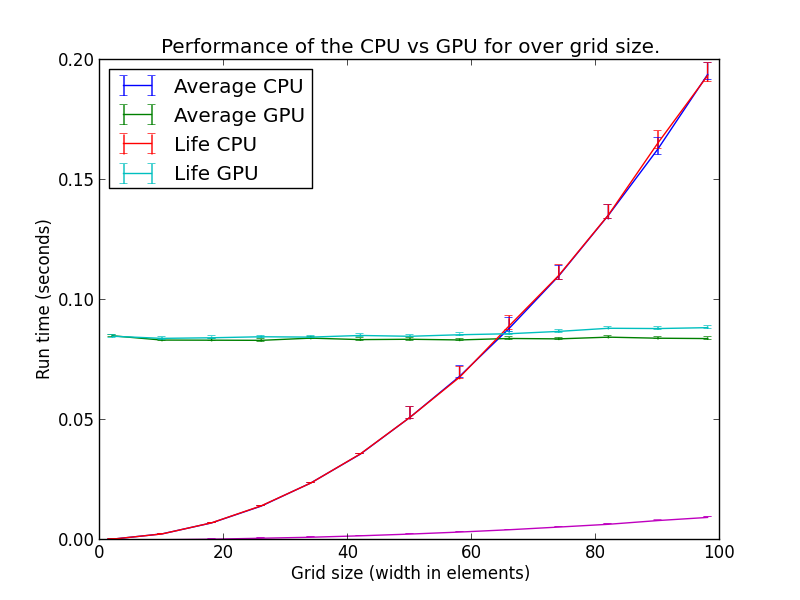
\includegraphics[width=\textwidth]{figs/run_performance.pdf}
  \caption{This plot shows the performance of the CPU versus the GPU
    implementations of the run primitive as it degrades with the grid size
    increasing. The grids are square in shape and the size given is for one of
    its dimensions. For comparison, both the average and game of life stencils
    are depicted. Also shown is the copy-on/off times for the GPU. Error bars
    are shown but most are vanishingly small.}
  \label{fig:runperf100}
\end{figure}

\begin{figure}[h]
  \includegraphics[width=\textwidth]{figs/run_performance2.pdf}
  \caption{This plot shows the performance of the GPU implementations of the run
    primitive as it degrades with a larger scale of grid size. Here we can see
    that both the Game of Life and average function diverge from the base
    measurement. Game of Life degrades the worst due to function calling
    overheads in its implementation. The CPU is not depicted as it grows too
    quickly, dwarfing the GPU measurements. }
  \label{fig:runperf1000}
\end{figure}

\begin{figure}[h]
  \includegraphics[width=\textwidth]{figs/run_performance3.pdf}
  \caption{Here we see the performance of the GPU on the same 0-1000 scale. Now
    the copy on/off time has been discounted by subtraction.}
  \label{fig:runperf1000dis}
\end{figure}

The results of the benchmarking showed that the GPU implementation outperforms
the CPU for grids of size greater than $30 \times 30$. This is in accordance
with the expected outcome, that the GPU is able to perform better modulo copy
on/off times.

On a scale of 0-100 (see \autoref{fig:runperf100}), the slowdown of the GPU
is barely visible above random variation. However, on a greater scale
(\autoref{fig:runperf1000}) it is clear that there is an increase in run
time.

The base measurement is the copy on/off time. We see that on the smaller scale
of analysis the base and actual stencils show little difference in performance
signifying that most of the time is spent in copying (between 20-50\% depending
on the stencil). On the greater scale we see how the stencil computations
actually diverge from the base as GPU computation time starts to become
significant. This can be seen more clearly in \autoref{fig:runperf1000dis}
where the copy on/off time has been discounted.

From the graphs we see that copy on/off time does not account for all the
overhead in the GPU computation. I hypothesise that this is due to a copy on/off
time for code as well as data (which was not accounted for in my
calculations). This is supported by the fact that the Game of Life has a greater
overhead at zero than the average function, because the implementation has
greater code size.

\subsubsection{Reduce}

\begin{figure}[h]
  \includegraphics[width=\textwidth]{figs/reduce_performance.pdf}
  \caption{This plot shows the performance of the CPU versus GPU versions of a
    reduction function. The reduction function given in this case in the sum
    function.}
  \label{fig:reduceperf}
\end{figure}

As we can see from \autoref{fig:reduceperf}, the performance of the reduce
primitive on the GPU also exceeds that of the CPU at $80\times80$ grid
size. This is a consequence of the fact that the reduction calculations are much
less intensive than those of the stencil function or the Game of Life.

\subsection{Deducing a model}

A future goal of this project might be to automatically decide when a certain
workload is best suited to the CPU or GPU. The experiments in this section have
already given us an insight into this: once grid size goes beyond a certain
size, the GPU should be used. We also saw that the complexity of the program
contributes to both the overhead and the scalability. However, at small values
of grid size the overhead of the GPU is most significant and so the degradation
can be ignored.

In order to deduce a model which could be used for switching between CPU and GPU
we must determine (a) an approximation function for the CPU's scalability, which
is mostly dependent on the grid size and (b) the overhead particular to our
program on the GPU, which depends on compiled code size as well as the grid
size. We will ignore (b) seeing as the evaluation was not sufficient to
determine this. (a) can be found by fitting a quadratic to the curve. This has
been done in \autoref{fig:fitting} and we can see that the quadratic
polynomial fits almost perfectly. The coefficients of this polynomial are given
by~\autoref{eq:quad}

\begin{equation} \label{eq:quad}
y = a x^2 + b x + c
\end{equation}
In this equation we can interpret $c$ as being the overhead for the CPU. The
coefficients are:
\begin{align*}
a & = & 3.23223432 \times 10^{-6}\\
b & = & -9.23861372 \times 10^{-6}\\
c & = & 1.56150424 \times 10^{-4}\\
\end{align*}

Knowing the particular overhead of our function, y, (as we have assumed) we are
now able to use \autoref{eq:quad} to calculate the grid size, $x$, for
which we should switch to using the GPU. We set $y$ to the run time of the GPU
operation (which we assumed is constant). Take $y=1.54 \times 10^{-3}$, as is
the case for the average stencil, then we get the resultant switching grid size
$x=22.17$ which agrees with the graph in \autoref{fig:runperf100}.

\begin{figure}[h]
  \includegraphics[width=\textwidth]{figs/run_performance_fit.pdf}
  \caption{Least square error fitting of a linear and quadratic curve to the
    performance data for the CPU implementation of the average function.}
  \label{fig:fitting}
\end{figure}

\section{Correctness}
\label{sec:correctness}

A central goal of the project was to produce a correct translation from Ypnos to
Accelerate. Already, by choosing a type safe language such as Haskell I vastly
reduced the number of run-time errors. To catch the rest I made use of
\emph{unit testing} and \emph{Test Driven Development} (TDD,
\autoref{sec:tdd}). Clearly, unit testing can only provide a partial assurance
of correctness and not a guarantee. However, I decided that a formal proof
(which could give these guarantees) was beyond the scope of this project. In
writing these tests I have assumed that the original CPU implementation was
correct and could be compared against as a gold standard\footnote{However, in
  running my tests I uncovered a bug in the implementation of boundaries which
  had to be fixed before this assumption could hold.}.

The testing framework used works slightly differently to other unit testing
frameworks. In a standard framework the user provides test cases which
incorporate both the test data (sometimes generated) and assertions. In
Haskell's \emph{QuickCheck} we only provide axioms about our functions and let
the framework provide the data based on the type.

Typically, QuickCheck will generate hundreds of test samples to verify a
particular axiom. This provides a better assurance than ordinary unit
testing as, via the random process, QuickCheck often comes up with corner
cases the programmer may not have devised themselves.

The following sections of my project required unit testing:

\begin{itemize}
\item The centring algorithm for grid patterns, as this contains a large part of
  the translations complexity.
\item The \texttt{funGPU} quasiquoter.
\item The \texttt{run} primitive.
\item The \texttt{reduce} primitive.
\end{itemize}

The approach taken to testing the grid patterns was to ensure that the
transformation:

\begin{itemize}
\item
  Starts with a grid that has certain properties (a precondition):
  regular size, positive size, has a cursor.
\item
  Maintains the regularity of size: the length of each row is the same.
\item
  Centres the cursor, given the original grid had a cursor.
\item
  Both roffset and coffset are always positive on such a grid (see
  \autoref{sec:centring} for an explanation of these two values).
\end{itemize}

The assumption was that grid patterns given to the transformation procedures
would be correct to begin with. As such, to improve the amount of test data
generated, I enforced these properties at the generation level. This is safe as
the grid patterns are generated through the CPU translation which I was assuming
to be correct.

To test the primitives I used a standard testing approach of comparing against a
reference implementation. For the \texttt{reduce} primitive I compare against
Haskell's built-in reduce function as I can safely assume this to be
correct. For the \texttt{run} primitive I originally intended to test against
the Ypnos CPU implementation.

The run primitive is tested by running the average function on a randomly
generated grid. The grid is passed to the GPU and CPU implementations of
\texttt{avg}. The resulting grid is then compared between the two and any
difference counts as a failure.

The same procedure is used for the reduce primitive. We use a one-dimensional
grid for this case as the built-in Haskell function we are comparing against is
one-dimensional. The resulting reduced values are compared and a failure is
registered if they should differ.

\section{Usability}

While not mentioned in my original proposal, the usability to the programmer is
another non-functional requirement. This project lacked time for a full
usability study. Instead, evaluated the usability using the method of
\emph{Cognitive Dimensions}~\cite{green96}, to compare the various approaches
already discussed.

Cognitive Dimensions of notations (CD) provide a light-weight vocabulary for
discussing various factors of programming language design. As Ypnos is
essentially a programming language (albeit, one embedded in Haskell) it makes
sense to use this technique. It works by specifying a number of properties of a
notation (\emph{dimensions}, a complete list can be found in
Green\cite{green96}) which must, in general, be traded off against one
another. For this reason it is important to understand the representative tasks
and the user that will be performing them. Then design decisions in the language
can be compared and evaluated using the dimensions relative to the tasks.

\subsection{System = Language + Environment}

It is important to note that CD relates to a whole system, not just the
language. We define the system to be the combination of programming language and
the programming environments. For example, programming over the phone versus
programming in a visual editor. For the purposes of discussing only the language
changes that I have introduced I will fix the environment and assume that it has
the following features:

\begin{itemize}
\item
  Screen-based text editor (e.g.~Vim, Emacs or TextMate)
\item
  Search and replace functionality (including regular expressions)
\end{itemize}

\subsection{Methodology}

I used the following procedure in evaluating the changes to Ypnos using
CD:

\begin{itemize}
\item
  Identify the relevant users of my system and sketch out a basic user
  profile.
\item
  Select the relevant task of these users on the part of the language I
  implemented.
\item
  Highlight which cognitive dimensions are most important to the selected tasks.
\item
  Show a comparison of the various approaches to this implementation.
\item
  Conclude which approach was taken and why.
\end{itemize}

\subsection{User profiles}

I have decided that given the applications to scientific computing and graphics,
the two main types of users would be scientists simulating physical systems and
graphics programmers developing graphics algorithms. I have included two user
stories for our two representative users:

\begin{shadequote}
  Kiaran is a physical scientist who is writing a simulation of a fluid dynamics
  system. He has a little Haskell experience already but has mostly used other
  languages such as Matlab and Fortran. He chose Ypnos/Haskell because he knew
  it would allow him to easily switch between a CPU implementation on his
  machine and a GPU implementation on the simulation machine he is using.
\end{shadequote}

\begin{shadequote}
  Noemi is writing a graphics transformation for a photo editing package. The
  photos her users edit are typically very large but she still would like to
  provide real-time performance with her algorithms. Noemi has a GPU in her
  computer, so she will be writing for this to ensure that her performance is
  good. However, she also wants her system to work on machines that do not have
  a compatible GPU. She already has experience in Haskell and is familiar with
  more complex features and extensions such as type and data families. She has
  picked Ypnos/Haskell because of its syntax and multiple backends.
\end{shadequote}

We can see that there are many tasks that these users would want to
perform with our system: coding up a filter into a stencil (Noemi),
writing a complex reduction to determine the state of the system
(Kiaran), debugging to find out why they get the wrong values (both).
However, I will be ignoring all tasks that involve parts of the system
which I did not implement. This leaves us with one central task for the
two use cases: converting between GPU and CPU.

The cognitive dimensions relevant to this task are:

\begin{tabular}{p{0.35\textwidth} p{0.6\textwidth}}
  Low repetition viscosity & to allow the programmer to easily change the
  implementation without changing too many points in code.
  \\
  Little to no imposed lookahead & allowing the programmer to use one
  implementation without having to think about later switching.
  \\
  Consistency & the programs syntax or usage does not change from CPU to
  GPU, e.g. changing only constructor names.
  \\
  Terseness & the syntax to specify the implementation does not get in the
  way of coding the stencils.
  \\
  Closeness of mapping & the model presented to the programmer through the API
  should map well to their mental model for these types of operation,
  e.g. comonadic operations.
  \\
\end{tabular}

The various approaches to provide an API to the programmer were discussed in the
\autoref{chap:impl}. They essentially boiled down to the following three
approaches: choosing the different implementation based on importing (also
called the non-unifying approach, see \autoref{sec:non-unify-appr}), using
type classes with associated data families (\autoref{sec:assoc-data-fam})
and using type classes with associated type families
(\autoref{sec:assoctypefam} and \autoref{sec:final}). For the sake of
comparison I will also include the approach of the programmer re-coding their
implementation in Accelerate for the GPU.

The results of the evaluation are briefly summarised in
\autoref{tbl:cogcompbrief}, for a full discussion see \autoref{tbl:cogcomp}
in the Appendix. An informal usability analysis such as this one was performed
at the end of each iterative development phase in order to inform the next
prototype.

\begin{longtable}{r | l l l l}
\hline

CD & Accelerate & Non-unifying & Data families & Type families

\\ \hline

Repetition viscosity & \textbf{Worst} & & & \textbf{Best}
\\

Imposed lookahead & \textbf{Worst} & \textbf{Best} & \textbf{Best} &
\textbf{Best}
\\

Consistency & \textbf{Worst} & & & \textbf{Best}
\\

Terseness & \textbf{Worst} & & & \textbf{Best}
\\

Hidden dependencies & \textbf{Best} & \textbf{Worst} & \textbf{Best} &
\textbf{Worst}
\\

Abstraction gradient & \textbf{Best} & & &
\\

Closeness of mapping & \textbf{Best} & \textbf{Worst} & \textbf{Worst} &
\textbf{Worst}
\\
\hline

\caption{A short comparison of the different APIs using cognitive
  dimensions. \label{tbl:cogcompbrief}}
\end{longtable}

\subsection{Discussion of Usability}

As we now can see, the best approach for our users is that of associated type
families with the data constructor for the stencil function. This approach is
best in the viscosity, imposed lookahead, consistency and terseness
dimensions. However, for this it has compromised in hidden dependencies,
abstraction and closeness of mapping.

The \emph{hidden dependency} problems are mitigated by the Haskell compiler
which warns and throws errors when there is a conflict in these dependencies,
e.g. if the user uses different \texttt{Sten} type constructors on the same grid
(see \autoref{lst:stendatafam}). While a little increase in hidden
dependencies is necessary to reduce viscosity, there could be room for
improvement here by making the types more consistent. This would help us remove
the dependencies due to the changing types and constraints.

Given that our example users are fairly advanced, the increase in
\emph{abstraction} should not be a problem, however, we should be aware of this
extra difficulty to learning the language. Advanced features such as type
families are hidden from the users in most cases, so Kiaran should not have a
problem.

The \emph{closeness of mapping} is an issue that is not inherent in the
implementation, but rather an artifact of it. With more time on this
project I would try to re-introduce the comonadic types to the type
family approach. This could require using a lower level implementation
rather than using Accelerate. For this reason getting a closer mapping
was beyond the scope of this project.

\section{Summary}

In this chapter we saw how the performance of my GPU implementation surpasses
that of the CPU for larger grid sizes. This holds for both the run and reduce
primitives. I demonstrated the testing approach taken and discussed how this can
provide some assurance as to the correctness of the translation. Finally, I
conducted usability evaluation using the method of cognitive dimensions.

In summary, this chapter demonstrated all the requirements of the project
(\autoref{sec:reqanal} and original proposal in \autoref{chap:prop}) have been
fulfilled:
\begin{enumerate}
\item Compilation of Ypnos code and implementation of the run primitive on the
  GPU.
\item Implementation of the reduce primitive on the GPU.
\item Better scaling than the current single threaded implementation when
  accounting for copy-on/off times.
\item The translation correctly preserves the semantics of Ypnos.
\end{enumerate}

Furthermore, I have demonstrated the usability of my API, a goal which was not
originally stated.

\chapter{Conclusion}

During this project I have learnt a large number of new and complicated
technologies from a field of computer science previously unknown to me. Having
only experienced the ML functional programming from Part Ia, diving into
Haskell's intricate type system has been an enlightening experience which has
taught me much about my personal software engineering approach and the type
systems of other languages.

\section{Accomplishments}

In this project I have managed to accomplish all the goals laid out by the
original proposal: a correct translation and run primitives which out-perform
their CPU counterparts. Furthermore, I conducted usability evaluation which was
not originally conceived as a requirement.

Aside from the mechanical goals of the project I have also deepened my own
knowledge of computer science and software engineering. I can now add Haskell to
the list of languages I am intimately familiar with. My experience with Haskell
has given me a better understanding of the type theoretic decisions that
underpin other more common languages (such as the various types of polymorphism
used in OOP). Furthermore, my software engineering approaches have been improved
by often needing to re-factor code and design complex systems such as the
centring algorithm.

I consider the project a success in that it both accomplished the requirements
(see \autoref{chap:evaluation}), providing a step forward for the Ypnos
programming language, and helped me learn much about Haskell and GPU
computation.

\section{Lessons Learnt}

In completing this project I have learnt the importance of having a strong plan
to stick to. I realised as I went further into this project that I had not
allocated enough time to researching and learning a new programming
ecosystem. Particularly, I had severely underestimated the time it would take to
get familiar with the complex type theory underlying the Haskell compiler.

Furthermore, if I were to repeat the project I would set out better procedures
for making notes and documenting the project as it progressed. The time required
to compile all the information for the dissertation and understand the different
approaches taken in the implementation was significantly more than I had
previously anticipated. In future work I will endeavour to keep a more complete
diary with frequent reviews of all the work accomplished so far and how it all
fits together.

\section{Future Work}

While all the goals of this project have been achieved, the path of accelerating
Ypnos on the GPU is by no means complete. A number of extensions from the
original proposal still have not been attempted, which include:

\begin{itemize}
\item The \texttt{iterate} primitive which would allow more efficient execution
  of pipelined operations.
\item The \texttt{zip} primitive which would allow implementation of more
  complicated algorithms which require multiple parameters. This would allow
  programs such as \emph{Canny edge detection} to be implemented.
\end{itemize}

Further to the original extensions, during the course of the project more
possible avenues for exploration were discovered. Further exploration may be
possible in:

\begin{itemize}
\item
  Attempting to expose the comonadic nature of operations in the type given to
  the programmer.
\item
  Deducing a full model for the GPU computation overhead.
\item
  Automatic selection of the backend dependent on static program analysis.
\end{itemize}

\printbibliography[heading=bibintoc]

\appendix

\input{appendix.tex}

\end{document}
}

\usepackage{fancyheadings}
\pagestyle{fancy}

\title{GPU Accelerating the Ypnos Programming Language}
\author{Samuel Pattuzzi\\ Robinson College}
\date{\today}
%TC:endignore

\begin{document}
\frontmatter

\input{title.tex}

\listoftodos

\chapter{Proforma}

{\large
\begin{tabular}{p{0.3\textwidth} p{0.7\textwidth}}
  Name:               & \bf Samuel Pattuzzi                                 \\
  College:            & \bf Robinson College                                \\
  Project Title:      & \bf \thetitle \\
  Examination:        & \bf Part II Project, June 2013                      \\
  Word Count:         & \bf \wordcount                                      \\
  Project Originator: & D.A. Orchard                                        \\
  Supervisor:         & D.A. Orchard                                        \\
\end{tabular}
}

\section*{Original Aims of the Project}

Creating a backend to the Ypnos programming language to support GPU accelerated
computation. This will require the implementation of translation from the Ypnos
stencil syntax to GPU code. Furthermore, it will require, as a minimum, two
language primitives to be implemented: \emph{run} and \emph{reduce}. Both the
translation and primitives must be correct and, furthermore, outperform the CPU
implementation.

\section*{Work Completed}

The criteria set out in the proposal were met. A backend consisting of a
compilation stage and two primitives was implemented. The correctness of the
implementation was checked by unit testing and benchmarks showed that the
performance of the GPU backend exceeded that of the CPU. In addition, a
usability analysis of the library was performed.

\section*{Special Difficulties}

None.

\newpage
\section*{Declaration}

I, Samuel Pattuzzi of Robinson College, being a candidate for Part II of the
Computer Science Tripos, hereby declare that this dissertation and the work
described in it are my own work, unaided except as may be specified below, and
that the dissertation does not contain material that has already been used to
any substantial extent for a comparable purpose.

I give permission for my dissertation to be made available in the archive
area of the Laboratory's website.

\begin{tabbing}
\bigskip \\
Signed   \= \\
\medskip \\
Date \> \thedate \\
\end{tabbing}

\cleardoublepage
{
 \hypersetup{linkcolor=black}
\setcounter{tocdepth}{2}
\tableofcontents
}
\cleardoublepage


\mainmatter

\chapter{Introduction}

In this project I created a compiler\footnote{We take compiler to mean the
  translation from Ypnos AST to an intermediary and so not the whole compiler
  stack.} for the Ypnos programming language that targets modern GPUs (Graphical
Processing Units) allowing for massive speed-ups of programs in this
language. The language allows programmers to use a very concise syntax to
describe certain types of parallel grid operations. Using this syntax it is now
possible to target machines both with and without compatible GPUs.

\section{Motivation}

GPUs have always been excellent exploiters of SIMD parallelism for graphics
applications. In recent years, however, the GPU pipeline has become more general
than ever. Beyond just providing programmable shaders\footnote{A shader is a
  small program used in graphics applications for simulating lighting effects on
  scenes and objects.} the platform has been opened up, allowing general
programming of GPUs, such as video codec acceleration and even scientific
computing. The ubiquity and low cost of this hardware creates an opportunity for
researchers, professionals and hobbyists alike.

The programming model enforced by the APIs of a GPU can be a significant hurdle
to programming. The APIs of such general purpose GPU (GPGPU) tends to be
low-level but at the same time restricted in ways that may be unfamiliar to the
user. Particularly, memory access within a thread is limited to allow effective
parallelism.

An alternative to using these lowest level APIs is higher level computational
paradigms which expose the SIMD parallelism of a program. Often these paradigms
are not as powerful, but allow for very concise programs within a certain field
of interest. For example, in the field of scientific computing many operations
can be described in terms of matrix operations, so a matrix manipulation library
could expose the SIMD parallelism needed.

The approach taken in the Ypnos programming language is to target a type of
computation common to graphics algorithms and scientific models. By taking a
simple and easy to learn paradigm and combining it with a declarative API, Ypnos
is able to exploit as much SIMD parallelism as needed under the
surface.

Furthermore, Ypnos is back-end agnostic, meaning its programs can easily be
transported from a GPU to a multi-core CPU or even clustered computers. Prior to
this project, Ypnos supported only CPU execution; this project implements a GPU
backend.

\section{Related work}

Ypnos was originally proposed by Orchard et al.\cite{ypnos-damp10}, as a
language embedded within Haskell with a CPU prototype. Haskell supports GPU
computation via the Accelerate library~\cite{acc-damp11}. I will briefly
introduce the reader to both, giving a grounding for the work to come.

\subsection{Ypnos}
\label{sec:ypnos}

\begin{hflisting}[label={lst:ypsyn1},caption={A simple mean function. Computes
    the mean of the neighbourhood of cells.}, float=h]
avg2D :: Grid (Dim X :* Dim Y) a -> a
avg2D = [fun| X*Y:|_  a _|
                  |b @c d|
                  |_  e _| -> (a + b + c + d + e )/5|]
out = run avg2D in -- Running the stencil on `in' to produce `out'
\end{hflisting}

\emph{Stencil computations} are an idiom used in parallel programming.  They
comprise a \emph{kernel} (or \emph{stencil}) which is applied to each element of
an array\footnote{In Ypnos, arrays are known as \emph{grids} to abstract from
  the implementation details.} of data. The kernel computes a new value for an
array location using its old value and the old values of its neighbouring
cells. Convolutions are a well-known example of stencil computation. An example
stencil is given in \autoref{lst:ypsyn1}. A more in depth explanation is given
in \autoref{sec:introduction-ypnos}.

The idiom is particularly useful in the fields of graphical processing and
scientific computing, where some typical applications include Gaussian blur,
Laplacian of Gaussian (an example of differential equation approximation), edge
detection and many other filter based methods. In the scientific domain, they
are used in the simulation of physical systems via fluid, stress or heat
dynamics.

Ypnos is an \emph{embedded domain specific language} (EDSL) for stencil
computations embedded within the Haskell programming
language~\cite{ypnos-damp10, ypnos-dsl11}. This allows Ypnos to share much of
the syntax and implementation of its host language. Haskell is a particularly
good fit for stencil computations as its purity allows the programmer to write
parallel programs without worrying about the interaction and sharing of state.

\subsection{Accelerate}

\emph{Accelerate}~\cite{acc-damp11} is also an EDSL for the Haskell language.
It implements parallel array computations on the GPU. Modern GPUs provide vast
amounts of SIMD parallelism via general purpose interfaces (GPGPU). Accelerate
uses matrix operations to expose SIMD parallelism to the GPU. This model is
easier for a programmer with a mathematical background to understand and exploit
error free.

Accelerate primarily targets GPUs which support NVIDIA's CUDA extension for
GPGPU programming. The library uses algorithmic skeletons for online CUDA code
generation~\cite{cole1989}. It provides operations such as \texttt{map},
\texttt{zip} and \texttt{fold} and implements its own stencil convolution
function.

We will revisit Accelerate in \autoref{sec:intr-axle}.


\chapter{Preparation}

This chapter introduces the subject detail required to understand the subsequent
chapters of the dissertation. This includes a brief introduction to some of
Haskell's more advanced features, the Ypnos programming language and the
Accelerate library.

Furthermore, this chapter discusses some of the foundational planning and design
choices. This includes the analysis of the initial system requirements, choice
of tools, libraries, programming languages, as well as software engineering
methodology.

\section{Requirements Analysis}
\label{sec:reqanal}

\newcommand{\low}{\ding{108}}
\newcommand{\medium}{\low\low}
\newcommand{\high}{\low\medium}

\newcommand{\mc}[1]{\multicolumn{2}{p{8cm}|}{#1}}
\newcommand{\stripe}[1]{\hline\multicolumn{5}{c}{#1}\\\hline}
\newcommand{\tblheaders}[1]{#1\\ \hline}
\newcommand{\tick}{\ding{52}}

\begin{table}[h]
\centering
\caption{Categorization of the main project requirements. The \emph{Ext} column marks requirements which are considered extensions.\label{tbl:reqanal}}
\begin{tabular}{l l|l|l|l|l}
  \tblheaders{\mc{\textbf{Requirements}} & \textbf{Priority} & \textbf{Difficulty} & \textbf{Risk} & \textbf{Ext}}

  \stripe{\textbf{Functional}}

  \mc{Stencil compilation -- compilation of Ypnos stencil syntax to functions runnable on the GPU.} & \high & \high & \medium &  \\

  \mc{Primitive support -- implementation of the primitive functions on the GPU:} & & & \\
  & Run & \high & \medium & \medium &  \\
  & Reduce & \high & \medium & \medium & \\
  & Iterate & \low & \low & \low & \tick \\
  & Zip & \low & \high & \low & \tick \\

  \stripe{\textbf{Non-Functional}}

  \mc{Correct translation -- ensure that the stencil translation is correct.} & \high & \medium & \high & \\

  \mc{Better scaling than CPU -- verify that the GPU implementation outperforms the CPU implementation.} & \high & \medium & \medium & \\

  \mc{Usable API -- ensure that the API presented to the programmer is usable.} & \medium & \medium & \medium & \tick \\

\end{tabular}
\end{table}

Requirements analysis undertaken in the early stages of this project allowed me
to proceed smoothly and identify potential points of failure early. Each major
goal of the project was categorized according to priority, difficulty and risk
(see \autoref{tbl:reqanal}).

The \emph{priority} signifies the importance to the completion of the project:
essential requirements have been marked as high and optional extensions as
low. Other important factors not mentioned in the proposal have also been
included and marked as medium priority. The \emph{difficulty} gave an estimate
of how hard certain requirements would be to achieve and so help provide an
estimate of how much resource should be dedicated. The \emph{risk} embodies the
initial uncertainty about the implementation details. A high risk requirement is
one that could easily take more time than initially foreseen.

The goals were further divided into \emph{functional} and \emph{non-functional}
requirements. Functional requirements specify what had to be implemented and
built during the course of the project. Non-functional requirements specify how
the system should perform and be tested.

An extra requirement was introduced since the proposal, namely a \emph{usable
  API}. Practically, this means that converting between CPU and GPU
implementations of the same program should require minimal code changes.

High risk and high priority requirements needed special attention to prevent the
project from falling behind schedule. In scheduling the tasks, I took a
risk-driven approach: trying to implement the highest risk functional
requirements first and test the highest risk non-functional requirements
early. At the same time, to ensure compilation correctness I took a test-driven
approach to development. I will talk about this in more detail in
\autoref{sec:tdd}.

From the dependency analysis of \autoref{fig:task-dep} a clear ordering to
the tasks is visible. The following order was adopted for the project: stencil
compilation, correctness verification, essential primitives, evaluation,
extensions.

\begin{figure}[h]
  \centering
  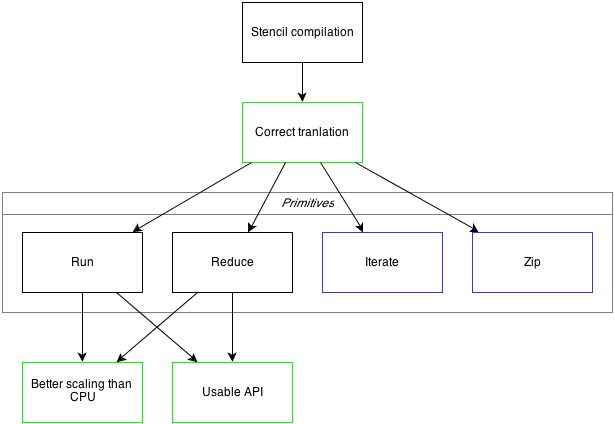
\includegraphics[width=\textwidth ]{figs/ypnos-task-dependency.pdf}
  \caption{This figure depicts the major task dependencies. The black boxes
    represent functional requirements, whereas the green boxes depict
    non-functional ones. Blue boxes are extensions.}
  \label{fig:task-dep}
\end{figure}

\section{Choice of Tools}

In this project I made use of both development tools, such as programming
languages and source control, as well as libraries for software reuse. Below, I
discuss the advantages and disadvantages of the tools, languages, and libraries
chosen

To familiarise myself with Ypnos, Accelerate and other tools, I started with
implementing sample functions in both. The main sample function was an average
stencil (which calculates the mean of its neighbour cell). Example code for this
stencil was given in \autoref{lst:ypsyn1} and will be discussed in detail in
\autoref{sec:introduction-ypnos}.

\subsection{Programming Languages}

Haskell was the obvious choice of programming language, given that Ypnos is
already developed in it. Having not programmed in Haskell before, I had to
become familiar with its more advanced features which were required by my
project (see \autoref{chap:impl}): \emph{type classes}, \emph{type families} and
\emph{data families}.

Haskell has excellent tools for developing compilers: strong typing, pattern
matching and mature parsing libraries
(Parsec\footnote{\url{http://hackage.haskell.org/package/parsec}}).
Furthermore, using the same language as the original implementation allowed for
much code reuse.

\subsection{Development Tools}

To aid the fetching of dependencies and the building of various targets I used
the \emph{Cabal} build system for
Haskell\footnote{\url{http://www.haskell.org/cabal/}}. Cabal features automatic
dependencies resolution and fetching as well as project building tools. By
writing some toy functions to test my knowledge of the Ypnos language I was also
able to set up a test build system in Cabal that I would later use in the rest
of my project. Cabal was chosen as it allowed me to automatically fetch and
install all the dependencies for my project as well as manage their versions and
compatibility.

\emph{Git} version control was used extensively throughout this project for
logging and backup. Although I was already quite familiar with this system, the
project allowed me to make use of some of Git's more advanced features such as
\emph{stashing}, \emph{sub-projects} and \emph{branching}. It was chosen
primarily for these advanced features as well as tight integration with free
hosting services such as \emph{Github}. This allowed my project to be frequently
backed up to the cloud.

\subsection{Libraries}
\subsubsection{Accelerate}

\emph{Accelerate} is a Haskell library which provides GPU accelerated array
computations. It is the only GPU programming library in Haskell which is
sufficiently powerful for my needs.

I chose Accelerate because of the native Haskell support and stencil
operations. It allowed me to abstract away from compiling to low-level C code
and, instead, concentrate on translating to a more abstract and general API.

Accelerate is discussed further in \autoref{sec:intr-axle}.

\subsubsection{CUDA}

\emph{CUDA} is a General Purpose GPU platform for NVidia devices\cite{cuda}. It
is the oldest framework of its kind but has recently been joined by the more
cross-platform OpenCL. The reason I chose CUDA over OpenCL was that the library
support in Haskell had the most stable support for it (though some experimental
support for OpenCL also exists).

As I do not own a machine with a CUDA enabled graphics card, I was using a
remote machine located in the Computer Laboratory. The sample functions allowed
me to set up the machine with the drivers and configuration required in order to
run the Accelerate library.

\section{Software Engineering Techniques}

This section highlights the software engineering approach taken in the
development of this project.

\subsection{Iterative Development}
\label{sec:iterdev}

Given my unfamiliarity with Haskell and GPU programming I followed the
\emph{iterative} model~\cite{cockburn08} to integrate exploration with
development. The end goal is to satisfy the project requirements. This and the
time constraints are the limiting factors of the iterative cycle.

\begin{figure}
  \centering
  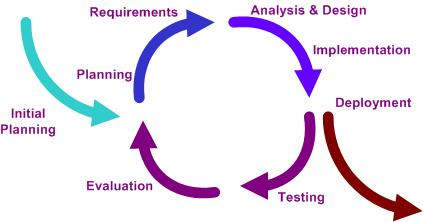
\includegraphics{./figs/Iterative_development_model_V2.jpg}
  \caption{One possible iterative development cycle. In the case of my project
    the deployment stage happened at the deadline and did not include a roll-out
    to actual customers. \\ \emph{Image courtesy of Wikipedia}}
  \label{fig:iterative}
\end{figure}

An iteratively developed project starts with an inception phase in which initial
requirements and goals are layed out. The project then proceeds through cycles
which consist of the following stages (see \autoref{fig:iterative}):

\begin{itemize}
\item
  Gathering requirements
\item
  Design
\item
  Coding
\item
  Testing
\item
  Evaluation
\end{itemize}

The first and last stages in the cycle merge together as requirements for the
next iteration feed off the examination of the last. After each cycle there is
an optional deployment phase in which the product is released. This phase is
omitted from the project.

Throughout the project various solution were attempted in phases and
re-evaluated based on issues found in the last iteration.  Iteration finished
when the requirements were met and the time limit reach.

\subsection{Test-Driven Development}
\label{sec:tdd}

The correctness of my implementation was a central goal. In order to achieve
this I took a test-driven approach to development: while writing the
implementation I was simultaneously writing unit tests for the code.  The
approach allowed me to quickly and effectively find bugs which had not already
been found by the Haskell type system.

\emph{QuickCheck} is the Haskell unit testing library\cite{claessen2011} used
throughout this project. QuickCheck and the testing methodology are discussed in
more detail in \autoref{sec:correctness}.

\section{Introduction to Ypnos}
\label{sec:introduction-ypnos}

Ypnos is an existing language with a fully formed syntax and a partial reference
implementation. Before I could start coding the translation from Ypnos to GPU, I
first had to understand and appreciate the reasoning behind the current choices
in the language and implementation.
\begin{figure}[!h]
\centering
% Define block styles
\tikzstyle{block} = [rectangle, draw,
    text width=6em, text centered, minimum height=4em]
\tikzstyle{ypnos} = [block, fill=blue!20]
\tikzstyle{haskell} = [block, fill=yellow!20]
\tikzstyle{bin} = [block, fill=gray!30]
\tikzstyle{surround} = [block, fill=gray!20]
\tikzstyle{line} = [draw, -latex']

\begin{tikzpicture}[row sep=0.5em]
  % Place nodes
  \def\x{7em}
  \node (9) {};
  \matrix[right=of 9] (1)
  {
    \node (title1) {Phase 1};\\
    \node [ypnos] (ypnos1) {Ypnos syntax}; \\
    \node [haskell] (haskell1) {Haskell code}; \\
    \node [ypnos] (libs) {Ypnos primitives}; \\
  };
  \matrix[right=\x of 1] (2)
  {
    \node (title2) {Phase 2}; \\
    \node [haskell] (haskell2) {Haskell code}; & \\
    \node [ypnos] (libs2) {Ypnos primitives}; & \\
  };
  \matrix[right=\x of 2] (3)
  {
    \node (title3) {Phase 3}; \\
    \node [bin] (bin) {Binary};\\
  };
  \begin{pgfonlayer}{background}
    \node [surround] (hasprim1) [fit = (haskell1) (libs)] {};
    \node [surround] (hasprim2) [fit = (haskell2) (libs2)] {};
    \node [surround] (background1) [fit = (title1) (hasprim1)] {};
    \node [surround] (background2) [fit = (title2) (hasprim2)] {};
    \node [surround] (background3) [fit = (title3) (bin)] {};
    \node [haskell] (hasprim1) [fit = (haskell1) (libs)] {};
    \node [haskell] (hasprim2) [fit = (haskell2) (libs2)] {};
  \end{pgfonlayer}
  % Draw edges
  \path [line] (background1) --
  node [midway, text width=6em, text centered, below] {Compile-time macros}
  (background2);
  \path [line] (background2) --
  node  [midway, below] {Compile} (background3);
\end{tikzpicture}
\caption{The compilation stages of an Ypnos program.\label{fig:comp-stages}}
\end{figure}

Ypnos consists of a library with various primitives used as the building blocks
of programs. Ypnos also provides some custom syntax via macros (see
\autoref{fig:comp-stages}).

\subsection{Grids}

The core data type in Ypnos is the \emph{grid}. As previously mentioned in
\autoref{sec:ypnos}, the grid is Ypnos' generalisation of the array. Unlike
the array, an Ypnos grid is implementation agnostic and could be implemented
differently with different backends.

Ypnos is designed with higher dimensions in mind so the grid may be
multi-dimensional (1D, 2D, etc.). In theory, the variable dimensionality of the
grids allows Ypnos stencil operations to be n-dimensional (although the
implementation doesn't currently support this).

\subsection{Parallelisation}

The stencil as a pattern is particularly good at exposing SIMD parallelism. On
systems like GPUs the amount of data sharing allowed is
restricted\footnote{Access to global shared memory (between thread blocks) is
  expensive. Instead thread block local memory should be used.}, which means
that operations on the different cores must be highly data parallel.

By \emph{subdivision} we are able to split a large grid into many subgrids (see
\autoref{fig:sten-decomp}). The stencils can operate over their subgrids in
parallel because the write-back points of each stencil never overlap. Therefore,
the stencils can safely read from a shared source grid.

\begin{figure}[h]
\centering
\begin{subfigure}{0.45\textwidth}
\centering
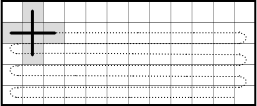
\includegraphics[width=0.95\textwidth]{figs/stencil-diagram.pdf}
\caption{Before subdivision}
\end{subfigure}
~
\begin{subfigure}{0.45\textwidth}
\centering
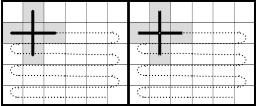
\includegraphics[width=0.95\textwidth]{figs/stencil-parallelised.pdf}
\caption{After subdivision}
\end{subfigure}
\caption{Subdivision of a grid for a 5-point stencil. The cursor location is
  shifted across the whole grid to produce a new grid.}
\label{fig:sten-decomp}
\end{figure}

\subsection{Stencil Syntax}

The Ypnos language provides a custom syntax for defining stencil functions as
well as a collection of primitive operations for their manipulation and use.

The code for a simple two dimensional averaging stencil is shown in
\autoref{lst:ypsyn2}.

\begin{hlisting}[label={lst:ypsyn2},caption={The simple mean function from \autoref{lst:ypsyn1}}]
avg2D :: Grid (Dim X :* Dim Y) a -> a
avg2D = [fun| X*Y:|_  a _|
                  |b @c d|
                  |_  e _| -> (a + b + c + d + e )/5|]
out = run avg2D in -- Running the stencil on `in' to produce `out'
\end{hlisting}

Compare this with the much more verbose imperative version of the same stencil
in \autoref{lst:avgimp}.  The \texttt{fun} macro is used to provide a
special \emph{grid pattern} syntax. The basic syntax of Ypnos can be summarised
as follows:

\begin{tabular}{p{0.1\textwidth} p{0.8\textwidth}}

  \texttt{X*Y:} & The syntax defines the dimensionality of the
  stencil. \texttt{X} and \texttt{Y} are both dimension variables (as is
  \texttt{Z}). They are combined usingthe \texttt{*} operator.  \\

\texttt{|} & The arguments are enclosed within pipe characters.  Their
arrangement in code is typically indented to reflect their grid shape.  \\

\texttt{a,b,\_} & Arguments can either be named or wildcard denoted
respectively with either a variable name or an underscore.  \\

\texttt{@} & This annotation denotes the variable is the cursor, the central cell whose position is used for the
result of the stencil (see \autoref{sec:primitives}).  \\

\texttt{->} & Delimiter that separates the grid pattern and the stencil body. It
appears to be normal Haskell syntax apart from recursion and function
definition.
\\

\end{tabular}

A generic stencil has a type of \texttt{Grid D a -> a} where \texttt{D} is the
dimensionality and \texttt{a} -- the element type. The dimensionality would take
the form \texttt{Dim X :* Dim Y} for a 2D grid.

\begin{hflisting}[label=lst:avgimp, caption={An imperative implementation of the
    average function. Note that the \texttt{in} index values have been laid out in the shape of the grid.}]
double in [M][N]; // Input array
double out [M][N]; // Output array
for (i = 1; i < M-1; i++){
  for (j = 1; j < N-1; j++){
    out[i][j] =
                 (in[i-1][j] +
     in[i][j-1] + in[i][j] + in[i][j+1]
                + in[i+1][j]) / 5;
  }
}
\end{hflisting}

\subsection{Primitives}
\label{sec:primitives}

As well as the syntax for stencil functions, Ypnos provides a library of
primitive operations. The primitives can be combined to create complex
accelerated computations over grids. The main primitive in Ypnos is \emph{run}
(see \autoref{lst:run-red}), which applies the stencil computation to a
grid.

\begin{hflisting}[label={lst:run-red}, caption={The basic \texttt{run},
\texttt{reduce} and, \texttt{reduceR} primitive as defined in the original Ypnos
paper\cite{ypnos-damp10}. \texttt{reduceR} provides a more general version of
the reducer allowing for intermediary values.}]

run :: (Grid D a -> b) -> Grid D a -> Grid D b

reduce :: (a -> a -> a) -> Grid D a -> a

reduceR :: Reducer a b -> Grid D a -> a
mkReducer :: exists b. (a -> b -> b)
                    -> (b -> b -> b)
                    ->  b
                    -> (b -> c)
                    -> Reducer a
\end{hflisting}

The application is done by moving the stencil cursor over each location in the
grid (we saw this illustrated in \autoref{fig:sten-decomp}). The arguments of
the stencil are taken from positions in the grid relative to the cursor. The
value is then computed using the specified computation and put into the same
cursor location in a \emph{new} grid.

In some locations near the edge of the grid there may not be enough neighbours
to satisfy a stencil. In this case Ypnos provides a special syntax for dealing
with these \emph{boundaries}. The implementation of boundaries is beyond the
scope of this project. However, a brief description of their behaviour will aid
the reader's understanding.

For each boundary of the grid, outside of which the stencil may access, a value
is computed by a user defined function. The function may use the current
location index and values from the grid (accessed via a specially bound
variable). A common boundary -- the \emph{mirror} boundary -- works by providing
the closest value inside the grid when an outside access is made. This is the
boundary that I have tacitly assumed to be default in my implementation.

Another vital primitive of the Ypnos language is the \emph{reduce} primitive
whose purpose is to summarise the contents of a grid in one value (see
\autoref{lst:run-red}). It may be used to compute functions such as the mean,
sum or minimum/maximum.

The primitive uses an associative operator (of type \texttt{a -> a -> a}) to
combine all the elements of the grid to one value. A more general version of
this operator, \emph{reduceR}, also exists (see \autoref{lst:run-red}),
which supports an intermediary type (or partial value).

The \emph{Reducer} data type takes the following parameters:

\begin{itemize}
\itemsep1pt\parskip0pt\parsep0pt
\item
  a function reducing an element and a partial value to a partial value,
\item
  a function reducing two partial values,
\item
  a default partial value
\item
  and a conversion from a partial value to the final value.
\end{itemize}

This Reducer is passed into the \emph{reduceR} primitive taking the place of the
associative operator in the reduce primitive. Clearly, reduce can be implemented
in terms of reduceR and so the latter is the more general.

\section{Introduction to Accelerate}
\label{sec:intr-axle}

We have already mentioned Accelerate as one of the implementors of stencil
convolution. In fact, Accelerate is an excellent target for intermediary code
compilation. While the stencil semantics of Accelerate and Ypnos differ in some
respects, the former is powerful enough to represent the latter. Therefore, the
project will target the Accelerate language instead of CUDA.

Accelerate uses the Haskell type system to differentiate between arrays
on the CPU and GPU. It does this by introducing a type encapsulating GPU
operations. There is a further \emph{stratification} of this type into
scalar and array values. Scalar computations may be composed into
array computations.

\subsection{GPU Computation}

For a process on the CPU to execute a CUDA program it must first send
the program and the data to the GPU. When the result is ready it must be copied
back into the main memory of the process concerned. I will call these two
procedure \emph{copy-on} and \emph{copy-off} respectively (see
\autoref{fig:copyonoff}).

\begin{figure}[tb]
  \includegraphics[width=\textwidth]{figs/copyonoff.pdf}
  \caption{An illustration of copy-on and copy-off times.  }
  \label{fig:copyonoff}
\end{figure}

Accelerate represents this difference in the type system. The \texttt{Acc} type
denotes an operation on the GPU. For the purposes of Accelerate, the only
operations allowed on the GPU are those over arrays. As such, \texttt{Array sh
  e} denotes an array of shape \texttt{sh} and element type \texttt{e}.
\texttt{Acc (Array sh e)} denotes the same but in GPU memory and encapsulate an
operation. This means that when such an array is evaluated a CUDA program must
be executed on the GPU.

Arrays are signalled for use on the GPU via the \texttt{use} primitive.  They
are copied-on, executed and copied-off via \texttt{run}. This primitive is
responsible for the run-time compilation and actual data transfer. All other
operations build an abstract syntax tree (AST) to be compiled by the
\texttt{run} primitive. Together \texttt{use} and \texttt{run} form the
constructors and destructors of the \texttt{Acc} data type (see
\autoref{lst:runuse}).

\begin{hflisting}[label={lst:runuse}, caption=The basic constructors and
  destructors for moving arrays too and from the GPU in Accelerate.]
use :: Array sh e -> Acc (Array sh e)
run :: Acc (Array sh e) -> Array sh e
\end{hflisting}

\subsection{Stratified Language}

The main form of operation in Accelerate is over arrays. However, it is often
desirable to build arrays out of multiple scalar values or functions over
scalars. A classic example of this is the map function which transforms an
entire array by a function over the individual values\footnote{In fact, the map
  function is conceptually similar to stencil application. The difference being
  that stencils take into account the neighbourhood of a cell to compute
  the next value whereas map takes only the central value.}(\autoref{lst:map}). For this reason, in addition to the \texttt{Acc} type,
Accelerate also provides the \texttt{Exp} type where the former represents
collective operations and the latter represents scalar computations. The two
types correspond to the two different types of AST built: one for scalar and the
other for array operations.

\begin{hflisting}[label={lst:map}, caption=The type of the \texttt{map}
  operation as defined by Accelerate.]
map :: (Exp a -> Exp b) -> Acc (Array sh a) -> Acc (Array sh b)
\end{hflisting}

Scalar operations do not support any type of iteration or recursion in order to
prevent divergent operation at run-time. However, most other Haskell code is
allowed. This is achieved by the Haskell type class mechanism (for ad-hoc
polymorphism, discussed further in \autoref{sec:typeclasses})-- Accelerate
provides instances of \texttt{Exp a} for most common classes.

For example, to support addition, subtraction and other numerical operations,
Accelerate provides an instance of the type class \texttt{Num}. This means that
operations can be typed as shown in \autoref{lst:num}.

\begin{hlisting}[label={lst:num}, caption=The type of addition overloaded by Accelerate.]
(+) :: Exp a -> Exp a -> Exp a
1 + 2 + 3 :: Exp Integer
\end{hlisting}

\subsection{Stencil Support}

Whilst \texttt{map} for an array applies a scalar function to every element in
an array, Accelerate provides support for running stencil computations via the
\texttt{stencil} function (see \autoref{lst:sten}).

\begin{hflisting}[label={lst:sten}, caption={The type of the stencil application
  function in Accelerate. Including an example instance of the
  \texttt{Stencil} type class. Many others are also possible.}]
stencil :: Stencil sh a sten =>
           (sten -> Exp b) ->
           Boundary a ->
           Acc (Array sh a) ->
           Acc (Array sh b)

instance Stencil DIM2 a ((Exp a, Exp a, Exp a)
                        ,(Exp a, Exp a, Exp a)
                        ,(Exp a, Exp a, Exp a))
\end{hflisting}

The first parameter is a function which represents the stencil. We see that
\texttt{sten}, the type of the stencil argument, takes the form of a tuple grid
of \texttt{Exp a} element type. This allows Accelerate to use Haskell's function
syntax to define stencils.

The second parameter is the type of boundary. In Accelerate, the types of
boundary allowed are fixed as opposed to Ypnos boundaries which can be fully
specified. One of the types allowed is \texttt{Mirror} (see
\autoref{sec:primitives}).

With these two parameters we have defined an operation which performs the
stencil convolution. An example stencil function is given in
\autoref{lst:ypsten}.

\begin{hlisting}[label={lst:ypsten}, caption={The ``average'' stencil defined
  using Accelerate's syntax.}]
avg :: Exp a => Stencil3x3 a -> Exp a
avg (( _, a, _ )
    ,( b, c, d )
    ,( _, e, _ )) = (a + b + c + d + e) / 5

type Stencil3x3 = ((Exp a, Exp a, Exp a)
                  ,(Exp a, Exp a, Exp a)
                  ,(Exp a, Exp a, Exp a))
\end{hlisting}

\section{Summary}

In this section we have seen an analysis of the project's requirements which
allowed me to prioritise the work for the project. Based on the requirements a
choice of tools and libraries was made. An iterative approach to development was
chosen to meet as many of the requirements as possible in the time given.

At the beginning of the project, time was spent on familiarisation with the
tools and libraries as well as the Ypnos language itself. Complex parts of the
Haskell language were investigated and understood (type classes and
families). The Accelerate library, central to the project, was investigated and
``toy'' programs were implemented in both Ypnos and Accelerate.

\chapter{Implementation}
\label{chap:impl}

The work of the implementation can be roughly split into two large chunks: the
compilation of stencils and the implementation of the primitives. In this
project I am aiming for both an accurate and fast translation as well as one
which is easy for the programmer to use.

In this chapter I will highlight the major implementation approaches taken for
the stencil compilation and primitives as well as an example usage of the
system.

\section{Iterative Development}

The iterative development approach was followed throughout the implementation of
this project. \autoref{tbl:iter} describes the phases of development: each
phase consisted of a working code prototype and a small usability evaluation. In
the following sections I will describe each approach taken in more detail.

\begin{table}
\begin{tabular}{l l | p{11cm}}
  \hline
  Phase 1 & Motivation & Create a working translation and run primitive using Accelerate.\\
  & Produced & The non-unifying approach to primitives and compile time approach to stencil translation with centring (\autoref{sec:non-unify-appr} and \autoref{sec:typesysapp}).
  \\
  Phase 2 & Motivation & Reduce the code changes the programmer must perform and unify the CPU and GPU run primitives.\\
  & Produced & The run and reduce primitives using type class parameters (\autoref{lst:redgrid})
  \\
  Phase 3 & Motivation & Make the return type of the reducer more useful to the user.\\
  & Produced & The run and reduce primitives using data families (\autoref{lst:rundatafam}).
  \\
  Phase 4 & Motivation & Remove the need for the programmer to change many constructors when switching.\\
  & Produced & The final approach using a combination of type synonym families and type class parameters (\autoref{sec:final}).\\
  \hline
\end{tabular}
\caption{The phase of iterative development in this project: for each cycle the motivation and work produced is described. \label{tbl:iter}}
\end{table}

\section{Stencil Compilation}

Compilation of stencils was a central task in this project. The abstract Ypnos
syntax is compiled down to Haskell AST to be run. Accelerate's implementation
has overridden much of the Haskell operators required for this translation
stage, so the bulk of the effort went into producing the functions that contain
the stencil computations. These functions take the form of
\autoref{lst:ypsten}

The arguments are formed as tuples of tuples. The rest of the stencil is normal
Haskell code. However, the return type, \texttt{Exp a}, ensures that all the
operations actually use Accelerate's overridden methods to build an AST. The AST
is then translated at run-time into CUDA code.

Ypnos achieves its custom syntax via Haskell's quasiquoting mechanism, a
language feature which allows the library author to provide custom syntax for
domain specific languages\cite{mainland2007}. The programmer must provide a
parser object (refered to as a quasiquoter). The essential function of a
quasiquoter is to provide an abbreviation for entering the AST manually.

Take, for example, the situation in which we want to write an embedded
language to act as a calculator. We have the AST for our
simple calculator in \autoref{lst:calc}.

\begin{hlisting}[label={lst:calc}, caption={A simple calculator defined using an
  AST (\texttt{Expr}) and using a quasiquoter for abbreviated syntax. The definition of
  \texttt{expr} is omitted.}]
data Expr  =  IntExpr Integer
           |  BinopExpr (Integer -> Integer -> Integer) Expr Expr

e1 = BinopExpr (+) (IntExpr 1) (IntExpr 3)
e2 = [expr| 1 + 3 |]
\end{hlisting}

We see that the quasiquoter \texttt{expr} allows us to abbreviate the expression
\texttt{e1} to the more obvious form of \texttt{e2}.

We could sensibly do the translation from Ypnos to Accelerate stencils in one of
two ways: we (a) use Haskell's type system to mask the difference between the
two operations at compile-time or (b) we use run-time compilation to mask the
difference between the implementations. Benefits and drawbacks of both are
presented in the next section.

\subsection{Centring}
\label{sec:centring}

One way in which Accelerate and Ypnos stencils differ is that the former assumes
that the cursor is at the centre of an odd sized grid ($3 \times 5, 5 \times 5$)
whereas the later allows the user to specify the centre. Ypnos stencils can be
translated to Accelerate stencils by padding the stencil passed to Accelerate
such that the cursor is centred.

Take an example: assume a one dimensional stencil with the cursor at an
off-centre location (denoted by \texttt{c}) -- \autoref{fig:cursor}.

\begin{figure}
  \centering
  \begin{subfigure}[t]{0.45\textwidth}
    \includegraphics[width=\textwidth]{figs/align1.pdf}
    \caption{The stencil before centring. Note the even shape ($4\times1$).}
    \label{fig:cursor}
  \end{subfigure}
  ~
  \begin{subfigure}[t]{0.45\textwidth}
    \includegraphics[width=\textwidth]{figs/align2.pdf}
    \caption{The same stencil after centring. Note the shape is now odd
      ($5\times1$)}
    \label{fig:centredcursor}
  \end{subfigure}
  \caption{Where $a$ is the position of the cursor and $b$ -- the length of the
    stencil.  In this diagram $pad_{start}$ represents the offset which needs to
    be applied to the centre, i.e the amount to pad the start of the
    grid. $pad_{end}$ represents the amount to pad the end of the grid. }
\end{figure}

Now we must determine the padding such that the cursor is centred. This is given
by the following two equations:

\[ pad_{start} = max \{a, b-a-1\} - a \]

\[ pad_{end} = max \{a, b-a-1\} - (b - a - 1) \]

This means that after centring we get \autoref{fig:centredcursor}

In order to implement the centring I had to consider both the one and two
dimensional cases.  It would be quite easy to deal with this in two separate
cases, except it must be possible to extend the approach to higher dimensions. I
considered three principle approaches to doing this: using lists as
intermediaries; using arrays as intermediaries; or operating on the grid
patterns directly via type classes.  Before addressing the approaches I will
mention the types in question (see \autoref{lst:gridpattern}).

\begin{hlisting}[label={lst:gridpattern}, caption=The data type which stores
  the grid patterns in Ypnos. Notice that the dimensionality is not exposed in
  the type but hidden.]
data GridPattern = GridPattern1D DimTag [VarP] |
                   GridPattern2D DimTag DimTag [[VarP]]
\end{hlisting}

\texttt{GridPattern} is the type in the Ypnos AST corresponding to the parsed
pattern of arguments. We see that it takes both a 1D and 2D form where the
variables (their type is \texttt{VarP}) are a list and a list of lists
respectively. We may also note that the dimensionality is expressed directly in
the constructor and as such is not present in the type.

The pattern of arguments in Accelerate is expressed as a tuple in the 1D case
and a tuple of tuples in the 2D case. This representation contains no explicit
information about which variables are cursors as we discussed in the previous
section.

\subsubsection{Type Classes}
\label{sec:typeclasses}

Haskell provides both \emph{parametric} and \emph{ad-hoc} polymorphism. The
former is provided by default in function definitions: each function is made to
work over the most general type possible. The latter is provided via the
mechanism of \emph{type classes}.  I required ad-hoc polymorphism in order to
operate differently on patterns of different dimensionalities.

A type class is declared in two parts: interface and instance. An interface has
a number of type parameters (also called indices) and function type
declarations. It is then possible to declare which types are instances of which
class. This is done by providing concrete types for the indices and concrete
definitions for the functions. \autoref{lst:typeclass} gives an example of a
type class declaration and instance.

\begin{hlisting}[label=lst:typeclass, caption={An example type class for
    equality. Showing the declaration and the instance for integers. Where
    \texttt{integerEq} is the implementation of integer equality on the target
    machine.}]
class Eq a where
  (==) :: a -> a -> Bool

instance Eq Integer where
  x == y =  x `integerEq` y

\end{hlisting}

\subsubsection{Type Families}
\label{sec:typefam}

Type families (also known as indexed type families) allow us to apply the same
kind of parameterisation as in type class to the
types\cite{chakravarty05}. Formally, type families are type functions from one
or more types to a single type. As with type classes there are both head
declarations and instances which define the family. The declaration describes
the \emph{``kind''}\footnote{A kind is the type theoretic name for a type for
  types. \texttt{*} denotes the kind of base types in Haskell.} of the family
and defines how many type arguments are taken.

Type families come in two flavours: data families and type synonym families. The
former allows the data type to be declared differently for different indexes,
whereas the latter allows different types to be synonymous.
\autoref{lst:datafam} gives an example of a data family being used to expose
the dimensionality of a pattern. This allows for the use of ad-hoc polymorphism
later on.

\begin{hlisting}[label=lst:datafam, caption=The data family declares tw<
  different constructors for 1D and 2D lists. The dimensionality of the list is
  exposed in the type.]
data family GridPatt :: * -> * -> *
data instance GridPatt (Int) a     = GridPatt1D Int [a]
data instance GridPatt (Int,Int) a = GridPatt2D (Int, Int) [[a]]
\end{hlisting}

Both flavours can be associated with a type class. In this case the index of the
type class must form part of the index of the type family. The interface and
instance declarations of the type family are bound to the corresponding
declarations of the type class. \autoref{lst:assoctypefam} gives an example
of an associated data family for patterns as opposed to it standing alone in
\autoref{lst:datafam}. The usage of type synonym families will be discussed
in detail in \autoref{sec:intr-type-class}.

\begin{hlisting}[label=lst:assoctypefam, caption={The data family from
    \autoref{lst:datafam} has now been associated with the class
    \texttt{GridIx} to provide the function \texttt{size} for various
    dimensionalities.}]
class (Ix i, Num i, ElMax i) => GridIx i where
    data GridPatt :: * -> * -> *
    size :: GridPatt i a -> i

instance GridIx (Int) where
    data GridPatt (Int) a = GridPatt1D Int [a]
    size (GridPatt1D s _) = s
\end{hlisting}

\subsubsection{Intermediate Approaches}

The first approach to centring taken involved first converting from grid
patterns into lists, then balancing these lists, and finally converting them
into the centred tuples needed for the Accelerate functional representation. In
order to do this I would have to define functions for measuring the location of
the cursor, and padding the lists before and after. This approach proved
difficult as lists did not explicitly incorporate their dimensionality in the
type. This made it hard to treat the 1D and 2D cases differently.

The second approach attempted to use existing array code in order to avoid
writing such functions. The hope was that by converting to arrays, rather than
lists, functions for appending and prepending rows and columns would already
exist. However, this was not the case and I would have had to write these
myself. As such, the intermediary array stage was not the best choice.

\subsubsection{Direct Approach}

The third and final approach was to operate directly on the lists extracted from
the \texttt{GridPattern} types. As previously mentioned, to retain
dimensionality information in the type system a type class was required.  I
designed a class \texttt{GridIx} (see \autoref{lst:gridix}) to perform the
basic operations -- \texttt{addBefore}, \texttt{addAfter}, \texttt{find} and
\texttt{size} -- in a dimension-sensitive way while still being polymorphic.

\begin{hlisting}[label={lst:gridix}, caption=The class declaration of
  \texttt{GridIx} showing the main functions defined for the grid manipulation
  and an associated data family.]
class (Ix i, Num i, ElMax i) => GridIx i where
    data GridPatt i :: * -> *
    addBefore :: i -> a -> GridPatt i a -> GridPatt i a
    addAfter :: i -> a -> GridPatt i a -> GridPatt i a
    find :: (a -> Bool) -> GridPatt i a -> i
    size :: GridPatt i a -> i
\end{hlisting}

The associated data type \texttt{GridPatt} would take the type of the particular
dimensionality of list that is appropriate for a given instance. In the case of
the index type \texttt{Int} we would get \texttt{GridPatt Int a = {[}a{]}} and
in the case of \texttt{(Int, Int)} we get \texttt{{[}{[}a{]}{]}}. This approach
allows the algorithms for centring to be described more generally regardless of
the number of dimensions actually involved.

This is the best and most efficient approach in terms of code reuse. This is why
I adopted this approach in the centring used for compile-time stencil
translation (described next).

\subsection{Compile-time Approach to Translation}
\label{sec:typesysapp}

As we saw in the previous section, the types of the Ypnos CPU stencil and the
Accelerate library's stencil differ wildly. \autoref{lst:avgsten} shows the
difference for the \texttt{avg}\footnote{For the sake of simplicity I have
  excluded the type constraints relating to boundaries as these are long
  and complicated.}  stencil.

\begin{hlisting}[label={lst:avgsten}, caption={The average function implemented
    on both the CPU and GPU. Note the difference in types. The constraints are
    simplified.}]
avgCPU :: (Array a, Floating a) => Grid (Dim X :* Dim Y) a ->     a
avgGPU ::      Floating (Exp a) =>            Stencil3x3 a -> Exp a
\end{hlisting}

In the GPU case we see that the type (once expanded) is tuples of tuples of
\texttt{Exp a}. On the other hand, in the Ypnos case we see that arguments take
the form of a grid, which is exactly the same type as the grids it operates on.

The Ypnos grid type is a \emph{comonad}, a functional programming design pattern
arising from Category Theory. The run primitive is an operation of the comonad,
\texttt{cobind} (\autoref{lst:cobind}).

\begin{hflisting}[label={lst:cobind}, caption={The definition of cobind. Let
    \texttt{D} be a grid of a certain dimension and \texttt{a} and \texttt{b} be
    the types of that grid.}]
cobind :: (D a -> b) -> D a -> D b
\end{hflisting}

The type system approach (or compile-time approach) means that Ypnos stencil
syntax is translated directly to a function with Accelerate type
(e.g. \texttt{avgGPU}) by using a different quasiquoter. This was implemented by
me in the \texttt{funGPU} quasiquoter (see \autoref{sec:usage} for usage
examples). Advanced type-system features in Haskell are used to unify the two
types of stencils. The pros and cons of this approach will be discussed in
\autoref{sec:prims}.

Unfortunately, by translating directly to the Accelerate stencil type we lose
the comonadic nature of the type. This is a shame, because this type is both
informative to the programmer (as it is a functional pattern), yet flexible
enough that by changing the instance of \texttt{D} we change the implementation.

The advantage of this method is that all the translation effort is done at
compile-time allowing the running of the stencil to be more efficient.

\subsection{Run-time Approach to Translation}
\label{sec:runtimetrans}

The second approach to the translation of stencils was to keep the types the
same as Ypnos' original implementation.  This is alluring as it allows us to
both expose more information to the user through the program's type and maintain
the theoretic underpinnings of Ypnos -- the comonadic structure. In order to
achieve this, some run-time conversions had to be done.

As already seen, we would like the \texttt{run} primitive to take the
form given in \autoref{lst:run2}

\begin{hflisting}[label={lst:run2}, caption=The comonadic run type. Changing the
  type of \texttt{g} could change the backend used.]
run :: Comonad g => (g a -> b) -> g a -> g b
\end{hflisting}

We have also seen that Accelerate does not accept stencils of this type (see
\autoref{sec:typesysapp}).  To solve this we previously broke the
comonadicity of the operation but we could attempt to preserve it by introducing
an \emph{arrow} data constructor to abstract the differences in type between the
notion of a stencil function\ in Accelerate and Ypnos. This changes the run
function to that seen in \autoref{lst:runarr}.

\begin{hlisting}[label={lst:runarr}, caption=The type run is generalised to
  using the \texttt{arrow} type.]
run :: Comonad g => (g a `arrow` b) -> g a -> g b
\end{hlisting}

The \texttt{arrow} constructor is parametrized on both \texttt{g a} and
\texttt{b}. To build up an instance of \texttt{arrow} we must pass in the
stencil function to a special constructor. The constructor chosen decides the
implementation used.

While previously (\autoref{sec:typesysapp}) we had to use different versions
of the quasiquoter to produce different stencils at compile-time, we now use the
same quasiquoter but convert the function at run-time. We achieve this by taking
advantage of Haskell's polymorphism which allows a function over type \texttt{a}
to specialise to a function of type \texttt{Exp a'}. This generalisation
combined with the arrow data constructor allows our stencil functions to have
the type in \autoref{lst:arrow-sten}

\begin{hlisting}[label={lst:arrow-sten}, caption=Here we see the type the
  stencil must have in Accelerate (\texttt{stencil}) and the type we can
  generalise to using the \texttt{arrow} type (\texttt{stencil'}).]
stencil :: Comonad g => g (Exp a) -> Exp b
stencil' :: Comonad g => g a `arrow` b
\end{hlisting}

Because of the arrow type, \texttt{stencil} and \texttt{stencil'} can now have
the same type.

The type of stencil accepted by Accelerate is still not of the form \texttt{g
  (Exp a) -\textgreater{} Exp b}. A conversion function builds an Accelerate
stencil (call it \emph{stencil A}) at run-time using the stencil encapsulated in
the arrow data type (call it \emph{stencil B}). Stencil A's arguments are used
to build up a grid of type \texttt{g (Exp a)}, then stencil B is used on this
grid to produce the result of type \texttt{Exp b}, finally this is returned as
stencil A's result. So stencil A behaves as a wrapper around stencil B.

While this run-time conversion creates an overhead, it also simplifies the types
significantly. A technique called deforestation may be used to mitigate the
overhead\footnote{Deforestation is also known as ``short cut fusion''. It is
  essentially an optimisation which eliminates intermediate data
  structures.}. Such optimisation is beyond the scope of this project due to
time constraints.

\section{Primitives}
\label{sec:prims}

The primitives are the second core component of the port to GPU. The
implementation of the primitives had two potential approaches: the first was to
re-implement the primitives in a separate module (a non-unifying approach). In
this case, the user would import whichever implementation they required. This
approach had some drawbacks -- for example, it required the user to change much
of their code between implementations.

This led to the second approach of extracting the functionality of the primitive
into a type class. This solution required the use of some complicated type
features in order to make the types unify. This lead to a further three
possibilities: (a) using a type class parameter for unification, (b) associating
a type family and (c) associating a data type.

The resultant approach was a hybrid of these. In this section I will detail all
the approaches taken and at the end of this section I will discuss the
trade-offs which lead to the final approach.

\subsection{Non-unifying Approach}
\label{sec:non-unify-appr}

The run primitive implemented in Phase 1 (see \autoref{tbl:iter}) used the
compile-time implementation of the stencil function
(\autoref{sec:typesysapp}). At the highest level this meant that the function
\texttt{run} had type given in \autoref{lst:runtype}.

\begin{hlisting}[label={lst:runtype}, caption=The type of run required by Accelerate.]
run :: (Stencil sh x sten) => (sten -> Exp y) -> Grid d x -> Grid d y
\end{hlisting}

However, we see that the type variable \texttt{sh} (required by Accelerate) and
\texttt{d} (required by Ypnos) do not unify requiring another constraint to
reconcile the two. Furthermore, constraints need to then be added for the types
of \texttt{x} and \texttt{y} to satisfy Accelerates \texttt{stencil}
function. In the end this type becomes unwieldy -- it is not straight-forward
for the user to write in their code.

Similar problems would have plagued the implementation of the \texttt{reduce}
primitive. However, having first seen the implementation of the \texttt{run}
primitive I decided that a different approach was necessary so this incarnation
of the \texttt{reduce} primitive was never implemented.

\subsection{Introducing Type Classes}
\label{sec:intr-type-class}

In this project I am aiming to make both an accurate and fast translation as
well as one which is easy for the programmer to use.  With the previous approach
we saw how this did not work for two reasons: (a) the run primitive I
implemented was not related (as far as Haskell was concerned) to the original
CPU primitive, and (b) the types of the two primitives differed, which could
cause compilation to fail if they were swapped.

The ideal would be a function which behaves differently under certain program
conditions. The perfect tool for this job is ad-hoc polymorphism which is
provided in Haskell via type classes (see \autoref{lst:avgsten}). The result is
an implementation of the primitive which changes dependent on a particular type
parameter. The obvious parameter in our case is the grid type, that is, have
different grid types for different backends.

We have seen this before: in some of the code examples I have used the notation
``Comonad g'' to refer to a grid which implements the primitives of Ypnos. This
was a type class approach. However, we run into the same problems as with
stencil translation (see \autoref{sec:runtimetrans}), namely the types of
stencil required by Accelerate and Ypnos differ.

\subsubsection{Type Class Parameter}

\begin{hflisting}[label={lst:redgrid}, caption={The \texttt{ReduceGrid} type
class defined with type parameters for each variable: \texttt{a}, \texttt{b} and
\texttt{c}. The \texttt{RunGrid} type class has type parameter \texttt{grid} and
\texttt{sten} where the later is fully determined by the former.}]
class ReduceGrid grid a b c | grid -> a,
                              grid -> b,
                              grid -> c where
    reduceG :: Reducer a b c-> grid -> c

data Reducer a b c where
    Reducer ::   (a -> b -> b)
              -> (b -> b -> b)
              -> b
              -> (b -> c)
              -> Reducer a b c

instance ReduceGrid CPUGrid a b c where
    reduceG = undefined -- Not implemented
instance ReduceGrid GPUGrid (Exp a) (Exp b) (Exp c) where
    reduceG = undefined -- Not implemented

class RunGrid grid sten | grid -> sten where
    runG :: sten -> grid -> grid

instance RunGrid CPUGrid CPUStencil
instance RunGrid GPUGrid GPUStencil
\end{hflisting}

The approach taken in Phase 2 to reconciling the stencil uses Haskell type
classes parametrized by more than one type. This allows us to abstract over
parts of the type that change to give a unified type. As the reduce primitive
was the first to bring about such issues, let's examine how this approach can be
applied to it (see \autoref{lst:redgrid}).

In this approach we are able to have instances for \texttt{Reducer} for the CPU
and GPU based on the grid type yet we also change the types of values accepted
by the functions of the Reducer. These types correspond to different types of
functions (\texttt{Exp a}) which tells Haskell to use Accelerate's overloaded
versions of operators.

We also see that the \texttt{RunGrid} type class is treated in a similar manner:
the type of grid uniquely determines the type of stencil function required. This
is achieved in Haskell using a \emph{functional dependency} (\texttt{grid ->
  sten}) meaning that the \texttt{grid} parameter uniquely determines the
\texttt{sten} parameter\cite{jones2000}. We see this a couple of times in the
given example.

Unlike the \texttt{reduceG} example, Haskell cannot, without help from the
programmer, choose a different quasiquoter (as is required with the static
approach as seen in \autoref{sec:typesysapp}).

\needspace{3\baselineskip}
In theory, this approach should work, however, it brings some usability
problems. Let's further examine the type of the \texttt{reduceG} primitive
when applied to \texttt{GPUGrid}s (see \autoref{lst:redgpu})

\begin{hflisting}[label={lst:redgpu}, caption={The type of the reducer once the
    Accelerate types are applied.}]
Reducer :: (Exp a -> Exp b -> Exp b)
        -> (Exp b -> Exp b -> Exp b)
        -> (Exp b) -- Default value
        -> (Exp b -> Exp c)
        -> Reducer (Exp a) (Exp b) (Exp c)
reduceG :: Reducer (Exp a) (Exp b) (Exp c)
        -> GPUGrid
        -> Exp c -- Return value
\end{hflisting}

Notice that both the return value and default value of the reducer have type
\texttt{Exp}, which is problematic, as \emph{lifting} and
\emph{unlifting}\footnote{Lifting is the process of promoting something of type
  \texttt{a} to type \texttt{Exp a}. Unlifting is the inverse process. Both
  aren't always possible.}  is not easy for the user to do and the wrapped value
is not particularly useful or meaningful once returned to the user. One approach
to changing this would be to introduce type parameters for the functions rather
than the values. However, the approach taken next offers greater flexibility.

\subsubsection{Associated Type Families}
\label{sec:assoctypefam}

We already encountered associated type families in
\autoref{sec:typefam}. Here we will be using type synonym families as
opposed to data families (Phase 4). These allow the unification of the different
function types required (see \autoref{lst:typesynfam} for an example of type
synonyms families unifying different function types).

\begin{hflisting}[label=lst:typesynfam, caption=The type synonym family is used
  as a type function. It is used to work out the element type of a collection.
  Here the \texttt{Fun} family (representing a one-argument function) can take
  two forms depending on the compilation target.]

type family Fun :: * -> * -> * -> *
type instance Fun CPUGrid a b = (a -> b)
type instance Fun GPUGrid a b = (Exp a -> Exp b)

\end{hflisting}

\needspace{7\baselineskip}
The ideal type for the \texttt{Reducer} in the GPU implementation is given in
\autoref{lst:reduceideal}

\begin{hlisting}[label={lst:reduceideal}, caption={The optimal type for the
    reduce primitive under Accelerate.}]
Reducer :: (Exp a -> Exp b -> Exp b)
        -> (Exp b -> Exp b -> Exp b)
        -> b -- Unlifted default
        -> (Exp b -> Exp c)
        -> Reducer a b c

reduceG :: Reducer a b c -> GPUGrid -> c -- Unlifted return
\end{hlisting}

\needspace{14\baselineskip}

This make the default easier to provide and result easier to use. By examining
this we can deduce that there are actually two types of abstract function
involved: 1- and 2-argument functions of \texttt{Exp}s. If we implement these as
two associated type families we get the behaviour required (see
\autoref{lst:redtypefam})

\begin{hlisting}[label={lst:redtypefam}, caption={The application of type
    families to the reduce primitive.}]
Reducer :: Fun2 g a b b
        -> Fun2 g b b b
        -> b
        -> Fun1 g b c
        -> Reducer g a b c

class ReduceGrid g where
    type Fun1 g a b
    type Fun2 g a b c
    reduceG :: Reducer g a b c -> g -> c
\end{hlisting}

Next I wanted to extend this approach to the run primitive. However, with run we
do not simply have a conversion of types, but also conditions on those types
(called constraints in Haskell). It is possible to encode constraints in a type
family method using a Haskell language extension called
\emph{ConstraintKinds}. This allows us to define a type family which has the
\emph{kind} of \texttt{Constraint} instead of the usual \texttt{*} (denoting
type as seen in \autoref{sec:typefam}). An example of the \texttt{RunGrid}
class modified in this way is given in \autoref{lst:constkind}.

\begin{hlisting}[label={lst:constkind}, caption={The application of type
    families to the run primitive.}]
class RunGrid g where
    type ConStencil g a b sten :: Constraint
    type Stencil g a b sten :: *
    run :: ConStencil g a b => (Stencil g a b) -> g x -> g y

instance RunGrid g where
    type ConStencil g a b sten = (Stencil sh a ~ sten, ShapeOf g ~ sh)
    type Stencil g a b sten = sten -> Exp b
\end{hlisting}

As we see, using associated type families is not general because we are exposing
\texttt{sten} -- a type variable which has no relevance to the CPU
implementation. Though it can be safely ignored, it exposes too much of the
underlying type difference which we are coding against and so does not decouple
the two implementations. As we will see in \autoref{sec:final}, this problem
can be mitigated by taking a hybrid approach.

\subsubsection{Associated data families}
\label{sec:assoc-data-fam}

Associated type families make the type of the stencil function explicit again
(Phase 3), as with the type class parameter. To achieve this we can make use of
associated data families (see \autoref{sec:typefam}). These work in much the
same way as type families, but rather than binding a particular synonym to a
class we bind a data type definition.

\autoref{lst:rundatafam} shows the \texttt{RunGrid} type class defined using
data families. We can see that the data family has replaced both the type and
constraint families from \autoref{sec:assoctypefam}.

\begin{hflisting}[label=lst:rundatafam,
caption=RunGrid with associated data family.]
class RunGrid g where
    data Sten g a b :: *
    runG :: Sten g a b -> g a -> g b
\end{hflisting}

This is done with \emph{generalized algebraic data types} (GADTs, another
Haskell type extension) which, amongst other things, allow us to place arbitrary
type constraints on constructors (\autoref{lst:stendatafam}).

\begin{hlisting}[label=lst:stendatafam,
caption={An example of a stencil data type for the GPU. Note the argument it takes is a stencil function (of type \texttt{sten -> Exp b}) where \texttt{sten} has been constrained in the required way.}]
data Sten (Array sh) a b where
        Sten :: (Shape sh, Stencil sh a sten,  -- constraints
                 Elt a, Elt b) =>              -- |
                (sten -> Exp b)
                -> Sten (Array sh) a b
\end{hlisting}

This allows for much cleaner implementation on our part but requires the
programmer to use different data constructors for the different implementations
(CPU versus GPU stencil functions). This is manageable when we are only dealing
with the different stencil types, however, if we add in the different types of
reduction function too, the programmer must make too many code changes.

\subsection{Final implementation}
\label{sec:final}

\begin{hflisting}[label=lst:final, caption={The final signatures of the
  \texttt{RunGrid} and \texttt{ReduceGrid} classes.}]
class RunGrid g arrow | arr -> g where
    type RunCon g arrow x y :: Constraint
    runG :: RunCon g arrow x y =>
            (x `arr` y)
            -> g x -> g y

class ReduceGrid g where
    type ConstFun1 g a b :: Constraint
    type ConstFun2 g a b c :: Constraint
    type Fun1 g a b
    type Fun2 g a b c
    reduceG :: Reducer g a c -> g a -> c
\end{hflisting}

The final implementation was a trade off between approaches. It combines the
type parameter for the \texttt{arrow} type\footnote{This is effectively the same
  as having used an associated data type, except a type synonym could be
  passed.} in the \texttt{RunGrid} class with associated type families for
constraints and generalized functions in the \texttt{ReduceGrid} class (see
\autoref{lst:final}).

The \texttt{RunGrid} class makes use of functional dependencies to ensure that
the \texttt{arrow} constructor the programmer specifies fully determines the
grid implmentation to be used. When using generalised constructors and
destructors (\autoref{sec:usage}) this means that if the programmer is
building their grids from lists then the correct implementation's grid will be
decided based on the \texttt{arrow} type used.

By using a type and not type synonyms for the stencil function I have eliminated
the need to expose a type variable in the declaration for type synonyms (as seen
in \autoref{sec:assoctypefam}). Now this can be neatly encapsulated within a
GADT.

\section{Usage}
\label{sec:usage}

The examples in \autoref{lst:example} are taken directly from the unit tests
for the application. They show the usage of the generalized constructors as well
as the \texttt{run} and \texttt{reduce} primitives. As we can see the user
doesn't have to deal with any of the types we mentioned previously.

\begin{hflisting}[label=lst:example,
caption=Usage of the final system taken from the unit tests.]

-- Take a list of integers and their dimensions and return the sum.
sum :: [Int] -> (Int, Int) -> Int
sum xs (x,y) =  reduceG (mkReducer (+) (+) 0 id) arr
    where arr = fromList (Z :. x :. y) (cycle xs)

-- Run a floating point stencil of any type
runF sten xs (x, y) = gridData (runG sten xs')
    where xs' = listGrid (Dim X :* Dim Y)
                         (0, 0) (x, y)
                         (cycle xs)
                         mirror

-- The average stencil for GPU
avgGPU = [funGPU| X*Y:|a  b c|
                      |d @e f|
                      |g  h i| ->
        (a + b + c + d + e + f + g + h + i)/9|]

-- The average stencil for CPU
avgCPU = [funCPU| X*Y:|a  b c|
                      |d @e f|
                      |g  h i| ->
        (a + b + c + d + e + f + g + h + i)/9|]

-- Run the average function on the GPU
runAvgGPU = runF (GPUArr avgGPU)

-- Run the average function on the CPU
runAvgCPU = runF (CPUArr avgCPU)

\end{hflisting}

\section{Summary}

Recall from \autoref{sec:introduction-ypnos} that Ypnos is a collection of
syntax extensions and a library of primitives. On top of the previous
implementation, this project implemented: changes to the syntax extensions to
allow the generation of GPU stencils (by implementing the \texttt{funGPU}
quasiquoter), library generalisation and API refinement, a re-factoring of CPU
primitives to fit the new API, and a set of new GPU primitives. See
\autoref{fig:files} for a complete summary of the changes introduced by this
project.

This chapter outlined: stencil compilation and the primitive implementation
(reduce and run). Stencil compilation was attempted in a compile-time and
run-time fashion with centring. Moreover, primitives were implemented in a
non-unifying way and then variously unified: type class parameters, associated
types and data families.

The pros and cons of each approach were discussed and at the end of the chapter
I described the final approach chosen. The chapter is rounded off with a brief
usage example for the translation, primitives, constructors and
destructors.

\begin{figure}[p]
\tikzstyle{every node}=[draw=black,thick,anchor=west]
\tikzstyle{created}=[draw=green,fill=green!30]
\tikzstyle{modified}=[draw=yellow,fill=yellow!30]
\begin{tikzpicture}[%
  grow via three points={one child at (0.5,-0.7) and
  two children at (0.5,-0.7) and (0.5,-1.4)},
  edge from parent path={(\tikzparentnode.south) |- (\tikzchildnode.west)}]
  \node {ypnos}
  child { node [created] {ypnos.cabal -- build file}}
  child { node [created] {benchmarks}
    child { node [created] {Benchmark.hs -- benchmark harness}}
    child { node [created] {Makefile}}
    child { node [created] {plot.py -- plotting functions}}
  }
  child [missing] {}
  child [missing] {}
  child [missing] {}
  child { node [] {src}
    child { node [] {Ypnos}
      child { node [modified] {Core -- modified to provide unifying types}
        child { node [] {Boundary.lhs}}
        child { node [modified] {Combinators.lhs}}
        child { node [] {Dimensions.lhs}}
        child { node [modified] {Grid.lhs}}
        child { node [] {Types.lhs}}
      }
      child [missing] {}
      child [missing] {}
      child [missing] {}
      child [missing] {}
      child [missing] {}
      child { node [created] {CUDA/Expr -- the core contribution}
        child { node [created] {Combinators.hs -- primitives}}
        child { node [created] {Fun.hs -- stencil translation}}
      }
      child [missing] {}
      child [missing] {}
      child { node [created] {Examples -- used for testing.}
        child { node [created] {Reductions.hs}}
        child { node [created] {Stencils.hs}}
      }
      child [missing] {}
      child [missing] {}
      child { node [modified] {Expr}
        child { node [] {Boundary.lhs}}
        child { node [] {Expr.lhs}}
        child { node [modified] {Fun.lhs}}
      }
    }
  }
  child [missing] {}
  child [missing] {}
  child [missing] {}
  child [missing] {}
  child [missing] {}
  child [missing] {}
  child [missing] {}
  child [missing] {}
  child [missing] {}
  child [missing] {}
  child [missing] {}
  child [missing] {}
  child [missing] {}
  child [missing] {}
  child [missing] {}
  child [missing] {}
  child [missing] {}
  child { node [created] {testsuite}
    child { node [created] {Test.hs}}
    child { node [created] {Testing/Ypnos/CUDA/Expr -- tests for all functionality implemented}
      child { node [created] {Combinators.hs}}
      child { node [created] {Fun.hs}}
    }
    child [missing] {}
    child [missing] {}
    child { node [created] {UnitTest.hs}}
  };

\end{tikzpicture}
\caption{The file tree of the final Ypnos project showing all work done. White
  files are unchanged from the original implementation. Green files are
  completely new and created by me. Yellow files were modified from the
  original.}
\label{fig:files}
\end{figure}

\chapter{Evaluation}
\label{chap:evaluation}

The main aims of this project were to produce a correct translation and speed up
over the CPU implementation (see \autoref{sec:reqanal}). In order to test
these two goals I have implemented unit tests throughout the course of this
project and implemented an evaluation suite of programs.

This section discusses the performance evaluation and measures taken to ensure a
correct translation. At the end of the chapter I will highlight the usability
evaluation conducted using the method of \emph{cognitive dimensions}.

\section{Performance}

Before the evaluation I postulated that the GPU should provide a speed up over
the CPU due to its capacity for parallel computation. More specifically, I
expected better scaling in the GPU case compared with the CPU.

\subsection{Methodology}

To measure the run-time I used the \emph{Criterion} library\cite{criterion}
which provides functions for:

\begin{itemize}
\itemsep1pt\parskip0pt\parsep0pt
\item Estimating the cost of a single call to the \texttt{clock} function.  The
  function that times the CPU and GPU.
\item Estimating the clock resolution.
\item Running Haskell functions and timing them discounting the above variations
  in order to get a sample of data.
\item Analysing the sample using \emph{bootstrapping}\cite{efron1981} to
  calculate the mean and confidence interval.
\end{itemize}

In my experimental setup I am using a confidence interval of 95\% and a sample
size (for bootstrapping) of 100 and a resample size of 100,000. The result from
Criterion is a mean with a confidence interval of 95\%. I will use these results
to compare the performance of the various functions implemented.

The machine being used for benchmarking was provided by the Computer Laboratory
and remotely hosted, with specifications:

\begin{itemize}
\itemsep1pt\parskip0pt\parsep0pt
\item
  Ubuntu Linux 12.04 64-bit edition
\item
  Quad core Intel Core i5-2400S CPU clocked at 2.50GHz with a 6M cache
\item
  16GB of core memory
\item Nvidia GeForce 9600 GT graphics card featuring 64 G94 cores with a 512 MB
  framebuffer.
\end{itemize}

\subsection{Overhead}

In order to show the speed-up, I must first discount the effects of copying to
and from the GPU\footnote{Though this is an important factor when considering
  CPU versus GPU, it was also a factor I could not control in this
  project. Therefore, I decided to discount it from my measurements.}. This was
done via an \texttt{identity} function implemented in Accelerate. The identity
function works by copying the data from the CPU to the GPU, performing no
operations on the GPU, then copying the data back. This will allow us to have a
base measure of how fast our computations run without overhead.

\subsection{Benchmark suite}

The benchmark suite must test the speed-up of both primitives: \texttt{run} and
\texttt{reduce}. I have implemented a set of representative functions for each
primitive to test speed across a representative set of calculations. These
functions include:

\begin{itemize}
\itemsep1pt\parskip0pt\parsep0pt
\item \textbf{The Average Stencil} (5-point version, \autoref{lst:example}) that
  we have seen in the previous sections. This function is representative of
  convolution style operations which we may wish to perform on the data. It
  operates over floating point numbers which is a common use case for scientific
  computing.
\item \textbf{The Game of Life Stencil} (\autoref{chap:life}) makes use
  of various boolean functions as well as (externally declared) functions used
  to count the number of \emph{true} values in a list.
\item \textbf{The Total Reducer} (\autoref{lst:example}) when normalised gives
  the mean which constitute one of the most common reduction operations over
  grids.
\end{itemize}

\subsection{Results}

\subsubsection{Run}

\begin{figure}[h]
  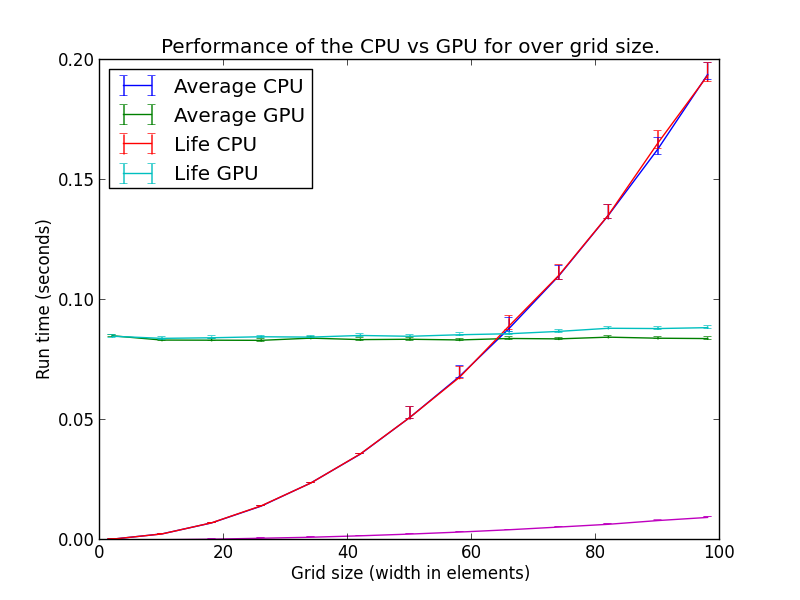
\includegraphics[width=\textwidth]{figs/run_performance.pdf}
  \caption{This plot shows the performance of the CPU versus the GPU
    implementations of the run primitive as it degrades with the grid size
    increasing. The grids are square in shape and the size given is for one of
    its dimensions. For comparison, both the average and game of life stencils
    are depicted. Also shown is the copy-on/off times for the GPU. Error bars
    are shown but most are vanishingly small.}
  \label{fig:runperf100}
\end{figure}

\begin{figure}[h]
  \includegraphics[width=\textwidth]{figs/run_performance2.pdf}
  \caption{This plot shows the performance of the GPU implementations of the run
    primitive as it degrades with a larger scale of grid size. Here we can see
    that both the Game of Life and average function diverge from the base
    measurement. Game of Life degrades the worst due to function calling
    overheads in its implementation. The CPU is not depicted as it grows too
    quickly, dwarfing the GPU measurements. }
  \label{fig:runperf1000}
\end{figure}

\begin{figure}[h]
  \includegraphics[width=\textwidth]{figs/run_performance3.pdf}
  \caption{Here we see the performance of the GPU on the same 0-1000 scale. Now
    the copy on/off time has been discounted by subtraction.}
  \label{fig:runperf1000dis}
\end{figure}

The results of the benchmarking showed that the GPU implementation outperforms
the CPU for grids of size greater than $30 \times 30$. This is in accordance
with the expected outcome, that the GPU is able to perform better modulo copy
on/off times.

On a scale of 0-100 (see \autoref{fig:runperf100}), the slowdown of the GPU
is barely visible above random variation. However, on a greater scale
(\autoref{fig:runperf1000}) it is clear that there is an increase in run
time.

The base measurement is the copy on/off time. We see that on the smaller scale
of analysis the base and actual stencils show little difference in performance
signifying that most of the time is spent in copying (between 20-50\% depending
on the stencil). On the greater scale we see how the stencil computations
actually diverge from the base as GPU computation time starts to become
significant. This can be seen more clearly in \autoref{fig:runperf1000dis}
where the copy on/off time has been discounted.

From the graphs we see that copy on/off time does not account for all the
overhead in the GPU computation. I hypothesise that this is due to a copy on/off
time for code as well as data (which was not accounted for in my
calculations). This is supported by the fact that the Game of Life has a greater
overhead at zero than the average function, because the implementation has
greater code size.

\subsubsection{Reduce}

\begin{figure}[h]
  \includegraphics[width=\textwidth]{figs/reduce_performance.pdf}
  \caption{This plot shows the performance of the CPU versus GPU versions of a
    reduction function. The reduction function given in this case in the sum
    function.}
  \label{fig:reduceperf}
\end{figure}

As we can see from \autoref{fig:reduceperf}, the performance of the reduce
primitive on the GPU also exceeds that of the CPU at $80\times80$ grid
size. This is a consequence of the fact that the reduction calculations are much
less intensive than those of the stencil function or the Game of Life.

\subsection{Deducing a model}

A future goal of this project might be to automatically decide when a certain
workload is best suited to the CPU or GPU. The experiments in this section have
already given us an insight into this: once grid size goes beyond a certain
size, the GPU should be used. We also saw that the complexity of the program
contributes to both the overhead and the scalability. However, at small values
of grid size the overhead of the GPU is most significant and so the degradation
can be ignored.

In order to deduce a model which could be used for switching between CPU and GPU
we must determine (a) an approximation function for the CPU's scalability, which
is mostly dependent on the grid size and (b) the overhead particular to our
program on the GPU, which depends on compiled code size as well as the grid
size. We will ignore (b) seeing as the evaluation was not sufficient to
determine this. (a) can be found by fitting a quadratic to the curve. This has
been done in \autoref{fig:fitting} and we can see that the quadratic
polynomial fits almost perfectly. The coefficients of this polynomial are given
by~\autoref{eq:quad}

\begin{equation} \label{eq:quad}
y = a x^2 + b x + c
\end{equation}
In this equation we can interpret $c$ as being the overhead for the CPU. The
coefficients are:
\begin{align*}
a & = & 3.23223432 \times 10^{-6}\\
b & = & -9.23861372 \times 10^{-6}\\
c & = & 1.56150424 \times 10^{-4}\\
\end{align*}

Knowing the particular overhead of our function, y, (as we have assumed) we are
now able to use \autoref{eq:quad} to calculate the grid size, $x$, for
which we should switch to using the GPU. We set $y$ to the run time of the GPU
operation (which we assumed is constant). Take $y=1.54 \times 10^{-3}$, as is
the case for the average stencil, then we get the resultant switching grid size
$x=22.17$ which agrees with the graph in \autoref{fig:runperf100}.

\begin{figure}[h]
  \includegraphics[width=\textwidth]{figs/run_performance_fit.pdf}
  \caption{Least square error fitting of a linear and quadratic curve to the
    performance data for the CPU implementation of the average function.}
  \label{fig:fitting}
\end{figure}

\section{Correctness}
\label{sec:correctness}

A central goal of the project was to produce a correct translation from Ypnos to
Accelerate. Already, by choosing a type safe language such as Haskell I vastly
reduced the number of run-time errors. To catch the rest I made use of
\emph{unit testing} and \emph{Test Driven Development} (TDD,
\autoref{sec:tdd}). Clearly, unit testing can only provide a partial assurance
of correctness and not a guarantee. However, I decided that a formal proof
(which could give these guarantees) was beyond the scope of this project. In
writing these tests I have assumed that the original CPU implementation was
correct and could be compared against as a gold standard\footnote{However, in
  running my tests I uncovered a bug in the implementation of boundaries which
  had to be fixed before this assumption could hold.}.

The testing framework used works slightly differently to other unit testing
frameworks. In a standard framework the user provides test cases which
incorporate both the test data (sometimes generated) and assertions. In
Haskell's \emph{QuickCheck} we only provide axioms about our functions and let
the framework provide the data based on the type.

Typically, QuickCheck will generate hundreds of test samples to verify a
particular axiom. This provides a better assurance than ordinary unit
testing as, via the random process, QuickCheck often comes up with corner
cases the programmer may not have devised themselves.

The following sections of my project required unit testing:

\begin{itemize}
\item The centring algorithm for grid patterns, as this contains a large part of
  the translations complexity.
\item The \texttt{funGPU} quasiquoter.
\item The \texttt{run} primitive.
\item The \texttt{reduce} primitive.
\end{itemize}

The approach taken to testing the grid patterns was to ensure that the
transformation:

\begin{itemize}
\item
  Starts with a grid that has certain properties (a precondition):
  regular size, positive size, has a cursor.
\item
  Maintains the regularity of size: the length of each row is the same.
\item
  Centres the cursor, given the original grid had a cursor.
\item
  Both roffset and coffset are always positive on such a grid (see
  \autoref{sec:centring} for an explanation of these two values).
\end{itemize}

The assumption was that grid patterns given to the transformation procedures
would be correct to begin with. As such, to improve the amount of test data
generated, I enforced these properties at the generation level. This is safe as
the grid patterns are generated through the CPU translation which I was assuming
to be correct.

To test the primitives I used a standard testing approach of comparing against a
reference implementation. For the \texttt{reduce} primitive I compare against
Haskell's built-in reduce function as I can safely assume this to be
correct. For the \texttt{run} primitive I originally intended to test against
the Ypnos CPU implementation.

The run primitive is tested by running the average function on a randomly
generated grid. The grid is passed to the GPU and CPU implementations of
\texttt{avg}. The resulting grid is then compared between the two and any
difference counts as a failure.

The same procedure is used for the reduce primitive. We use a one-dimensional
grid for this case as the built-in Haskell function we are comparing against is
one-dimensional. The resulting reduced values are compared and a failure is
registered if they should differ.

\section{Usability}

While not mentioned in my original proposal, the usability to the programmer is
another non-functional requirement. This project lacked time for a full
usability study. Instead, evaluated the usability using the method of
\emph{Cognitive Dimensions}~\cite{green96}, to compare the various approaches
already discussed.

Cognitive Dimensions of notations (CD) provide a light-weight vocabulary for
discussing various factors of programming language design. As Ypnos is
essentially a programming language (albeit, one embedded in Haskell) it makes
sense to use this technique. It works by specifying a number of properties of a
notation (\emph{dimensions}, a complete list can be found in
Green\cite{green96}) which must, in general, be traded off against one
another. For this reason it is important to understand the representative tasks
and the user that will be performing them. Then design decisions in the language
can be compared and evaluated using the dimensions relative to the tasks.

\subsection{System = Language + Environment}

It is important to note that CD relates to a whole system, not just the
language. We define the system to be the combination of programming language and
the programming environments. For example, programming over the phone versus
programming in a visual editor. For the purposes of discussing only the language
changes that I have introduced I will fix the environment and assume that it has
the following features:

\begin{itemize}
\item
  Screen-based text editor (e.g.~Vim, Emacs or TextMate)
\item
  Search and replace functionality (including regular expressions)
\end{itemize}

\subsection{Methodology}

I used the following procedure in evaluating the changes to Ypnos using
CD:

\begin{itemize}
\item
  Identify the relevant users of my system and sketch out a basic user
  profile.
\item
  Select the relevant task of these users on the part of the language I
  implemented.
\item
  Highlight which cognitive dimensions are most important to the selected tasks.
\item
  Show a comparison of the various approaches to this implementation.
\item
  Conclude which approach was taken and why.
\end{itemize}

\subsection{User profiles}

I have decided that given the applications to scientific computing and graphics,
the two main types of users would be scientists simulating physical systems and
graphics programmers developing graphics algorithms. I have included two user
stories for our two representative users:

\begin{shadequote}
  Kiaran is a physical scientist who is writing a simulation of a fluid dynamics
  system. He has a little Haskell experience already but has mostly used other
  languages such as Matlab and Fortran. He chose Ypnos/Haskell because he knew
  it would allow him to easily switch between a CPU implementation on his
  machine and a GPU implementation on the simulation machine he is using.
\end{shadequote}

\begin{shadequote}
  Noemi is writing a graphics transformation for a photo editing package. The
  photos her users edit are typically very large but she still would like to
  provide real-time performance with her algorithms. Noemi has a GPU in her
  computer, so she will be writing for this to ensure that her performance is
  good. However, she also wants her system to work on machines that do not have
  a compatible GPU. She already has experience in Haskell and is familiar with
  more complex features and extensions such as type and data families. She has
  picked Ypnos/Haskell because of its syntax and multiple backends.
\end{shadequote}

We can see that there are many tasks that these users would want to
perform with our system: coding up a filter into a stencil (Noemi),
writing a complex reduction to determine the state of the system
(Kiaran), debugging to find out why they get the wrong values (both).
However, I will be ignoring all tasks that involve parts of the system
which I did not implement. This leaves us with one central task for the
two use cases: converting between GPU and CPU.

The cognitive dimensions relevant to this task are:

\begin{tabular}{p{0.35\textwidth} p{0.6\textwidth}}
  Low repetition viscosity & to allow the programmer to easily change the
  implementation without changing too many points in code.
  \\
  Little to no imposed lookahead & allowing the programmer to use one
  implementation without having to think about later switching.
  \\
  Consistency & the programs syntax or usage does not change from CPU to
  GPU, e.g. changing only constructor names.
  \\
  Terseness & the syntax to specify the implementation does not get in the
  way of coding the stencils.
  \\
  Closeness of mapping & the model presented to the programmer through the API
  should map well to their mental model for these types of operation,
  e.g. comonadic operations.
  \\
\end{tabular}

The various approaches to provide an API to the programmer were discussed in the
\autoref{chap:impl}. They essentially boiled down to the following three
approaches: choosing the different implementation based on importing (also
called the non-unifying approach, see \autoref{sec:non-unify-appr}), using
type classes with associated data families (\autoref{sec:assoc-data-fam})
and using type classes with associated type families
(\autoref{sec:assoctypefam} and \autoref{sec:final}). For the sake of
comparison I will also include the approach of the programmer re-coding their
implementation in Accelerate for the GPU.

The results of the evaluation are briefly summarised in
\autoref{tbl:cogcompbrief}, for a full discussion see \autoref{tbl:cogcomp}
in the Appendix. An informal usability analysis such as this one was performed
at the end of each iterative development phase in order to inform the next
prototype.

\begin{longtable}{r | l l l l}
\hline

CD & Accelerate & Non-unifying & Data families & Type families

\\ \hline

Repetition viscosity & \textbf{Worst} & & & \textbf{Best}
\\

Imposed lookahead & \textbf{Worst} & \textbf{Best} & \textbf{Best} &
\textbf{Best}
\\

Consistency & \textbf{Worst} & & & \textbf{Best}
\\

Terseness & \textbf{Worst} & & & \textbf{Best}
\\

Hidden dependencies & \textbf{Best} & \textbf{Worst} & \textbf{Best} &
\textbf{Worst}
\\

Abstraction gradient & \textbf{Best} & & &
\\

Closeness of mapping & \textbf{Best} & \textbf{Worst} & \textbf{Worst} &
\textbf{Worst}
\\
\hline

\caption{A short comparison of the different APIs using cognitive
  dimensions. \label{tbl:cogcompbrief}}
\end{longtable}

\subsection{Discussion of Usability}

As we now can see, the best approach for our users is that of associated type
families with the data constructor for the stencil function. This approach is
best in the viscosity, imposed lookahead, consistency and terseness
dimensions. However, for this it has compromised in hidden dependencies,
abstraction and closeness of mapping.

The \emph{hidden dependency} problems are mitigated by the Haskell compiler
which warns and throws errors when there is a conflict in these dependencies,
e.g. if the user uses different \texttt{Sten} type constructors on the same grid
(see \autoref{lst:stendatafam}). While a little increase in hidden
dependencies is necessary to reduce viscosity, there could be room for
improvement here by making the types more consistent. This would help us remove
the dependencies due to the changing types and constraints.

Given that our example users are fairly advanced, the increase in
\emph{abstraction} should not be a problem, however, we should be aware of this
extra difficulty to learning the language. Advanced features such as type
families are hidden from the users in most cases, so Kiaran should not have a
problem.

The \emph{closeness of mapping} is an issue that is not inherent in the
implementation, but rather an artifact of it. With more time on this
project I would try to re-introduce the comonadic types to the type
family approach. This could require using a lower level implementation
rather than using Accelerate. For this reason getting a closer mapping
was beyond the scope of this project.

\section{Summary}

In this chapter we saw how the performance of my GPU implementation surpasses
that of the CPU for larger grid sizes. This holds for both the run and reduce
primitives. I demonstrated the testing approach taken and discussed how this can
provide some assurance as to the correctness of the translation. Finally, I
conducted usability evaluation using the method of cognitive dimensions.

In summary, this chapter demonstrated all the requirements of the project
(\autoref{sec:reqanal} and original proposal in \autoref{chap:prop}) have been
fulfilled:
\begin{enumerate}
\item Compilation of Ypnos code and implementation of the run primitive on the
  GPU.
\item Implementation of the reduce primitive on the GPU.
\item Better scaling than the current single threaded implementation when
  accounting for copy-on/off times.
\item The translation correctly preserves the semantics of Ypnos.
\end{enumerate}

Furthermore, I have demonstrated the usability of my API, a goal which was not
originally stated.

\chapter{Conclusion}

During this project I have learnt a large number of new and complicated
technologies from a field of computer science previously unknown to me. Having
only experienced the ML functional programming from Part Ia, diving into
Haskell's intricate type system has been an enlightening experience which has
taught me much about my personal software engineering approach and the type
systems of other languages.

\section{Accomplishments}

In this project I have managed to accomplish all the goals laid out by the
original proposal: a correct translation and run primitives which out-perform
their CPU counterparts. Furthermore, I conducted usability evaluation which was
not originally conceived as a requirement.

Aside from the mechanical goals of the project I have also deepened my own
knowledge of computer science and software engineering. I can now add Haskell to
the list of languages I am intimately familiar with. My experience with Haskell
has given me a better understanding of the type theoretic decisions that
underpin other more common languages (such as the various types of polymorphism
used in OOP). Furthermore, my software engineering approaches have been improved
by often needing to re-factor code and design complex systems such as the
centring algorithm.

I consider the project a success in that it both accomplished the requirements
(see \autoref{chap:evaluation}), providing a step forward for the Ypnos
programming language, and helped me learn much about Haskell and GPU
computation.

\section{Lessons Learnt}

In completing this project I have learnt the importance of having a strong plan
to stick to. I realised as I went further into this project that I had not
allocated enough time to researching and learning a new programming
ecosystem. Particularly, I had severely underestimated the time it would take to
get familiar with the complex type theory underlying the Haskell compiler.

Furthermore, if I were to repeat the project I would set out better procedures
for making notes and documenting the project as it progressed. The time required
to compile all the information for the dissertation and understand the different
approaches taken in the implementation was significantly more than I had
previously anticipated. In future work I will endeavour to keep a more complete
diary with frequent reviews of all the work accomplished so far and how it all
fits together.

\section{Future Work}

While all the goals of this project have been achieved, the path of accelerating
Ypnos on the GPU is by no means complete. A number of extensions from the
original proposal still have not been attempted, which include:

\begin{itemize}
\item The \texttt{iterate} primitive which would allow more efficient execution
  of pipelined operations.
\item The \texttt{zip} primitive which would allow implementation of more
  complicated algorithms which require multiple parameters. This would allow
  programs such as \emph{Canny edge detection} to be implemented.
\end{itemize}

Further to the original extensions, during the course of the project more
possible avenues for exploration were discovered. Further exploration may be
possible in:

\begin{itemize}
\item
  Attempting to expose the comonadic nature of operations in the type given to
  the programmer.
\item
  Deducing a full model for the GPU computation overhead.
\item
  Automatic selection of the backend dependent on static program analysis.
\end{itemize}

\printbibliography[heading=bibintoc]

\appendix

\chapter{Original Proposal}
\label{chap:prop}

\input{propbody.tex}

\chapter{Full Cognitive Dimension Analysis}
\label{chap:cogdim}

\newcommand{\sideways}[1]{
  \parbox[t]{2mm}{{\rotatebox[origin=r]{90}{#1}}}}
\newlength{\fstcollen}
\newlength{\sndcollen}
\setlength{\fstcollen}{0.5cm}
\setlength{\sndcollen}{(\textwidth-\fstcollen-2cm)/4}
\begin{longtable}{r | p{\sndcollen} p{\sndcollen} p{\sndcollen} p{\sndcollen}}
\hline\noalign{\medskip}

\sideways{CD}
 &
Accelerate
 &
Non-unifying
 &
Data families
 &
Type families (only stencil data type)

\\\noalign{\medskip}
\hline\noalign{\medskip}

\sideways{Repetition viscosity}
 &
\textbf{Worst}

Clearly here we have a very high viscosity: each function must be re-written in terms of new syntax and run in different ways.
 &
We have improved the viscosity significantly. The user must only
implement their stencils in one language but they must still change all
the imports and correct type errors.
 &
Data families worsen the viscosity over the import method as we must now
change all the data constructors as opposed to the imports. In real code
there will be more of these than import locations.
 &
\textbf{Best}

Here we have the least repetition viscosity of all the approaches. We
now only need to change the quasi quoter to change the whole
implementation.

\\\noalign{\medskip}

\sideways{Imposed lookahead}
 &
\textbf{Worst}

The user must know ahead of time that they will be writing in two
languages to be sure to minimize duplication of code and structure their
program correctly.
 &
\textbf{Best}

There is practially no imposed lookahead as we can simply swap out the
implementation by importing from different places.
 &
\textbf{Best}

We do not have imposed lookahead as we can easily swap the constructors.
 &
\textbf{Best}

There is little imposed lookahead in theory, though some operations are
currently not supported in the GPU implementation. (TODO: link to more)
Some types may not be supported easily in both implementations so this
should be considered too.

\\\noalign{\medskip}

\sideways{Consistency}
 &
\textbf{Worst}

The syntaxes are different and so are fairly inconsistent. There are,
however, some similarities between the two in their stencil
representation.
 &
Consistency is improved as the syntax is now uniform but types are not
uniform.
 &
The syntax and usage is the same except for changing the constructors
which is inconsistent.
 &
\textbf{Best}

We have eliminated the inconsistency in usage of the data families. Now
the approach is almost entirely consistent except for the types.

\\\noalign{\medskip}

\sideways{Terseness}
 &
\textbf{Worst}

A lot of code is written by the user to cope with the two different
implementations.
 &
Changing requires a fair bit of code to be changed as we may be
importing many different things from the Ypnos libraries and all these
things must be changed.
 &
We require a lot of code to express the swap from CPU to GPU.
 &
\textbf{Best}

The syntax for switching is minimally terse.

\\\noalign{\medskip}

\sideways{Hidden dependencies}
 &
\textbf{Best}

No hidden dependencies. It is very clear and explicit what is going on.
 &
\textbf{Worst}

Many hidden dependencies are introduced as the types of the different
imported functions do not necessarily match. This can cause failures in
many different places on changing the import.
 &
\textbf{Best}

Here the dependencies introduced in the type system by the import
approach have been made explicit by data constructors.
 &
\textbf{Worst}

More hidden dependencies are introduced. Types change without the users knowing
due to different type and constraint families. This might affect some programs.

\\\noalign{\medskip}

\sideways{Abstraction gradient}
 &
\textbf{Best}

The abstraction is at its most basic level -- choosing between Ypnos or
Accelerate. The user must get to grips with these abstractions as a
minimum.
 &
The abstraction level is fairly low as it uses only simple Haskell
constructs.
 &
The user must now be familiar with the idea of an associated data family
and GADT which are quite advanced Haskell type features.
 &

The abstraction here is perhaps highest of all as it uses the most
advanced type features.

\\\noalign{\medskip}

\sideways{Closeness of mapping}
 &
\textbf{Best}

This way we preserve the comonadic nature of the operations in the type
so that it is obvious to the user what is going on.
 &
\textbf{Worst}

The comonadicity is lost due to having to change the types to suit the
accelerate implementation.
 &
\textbf{Worst}

The comonadicity is lost also.
 &
\textbf{Worst}

The comonadicity is lost.

\\\noalign{\medskip}
\hline
\noalign{\medskip}
\caption{Comparison of the different API using cognitive dimensions. \label{tbl:cogcomp}}
\end{longtable}


\end{document}
}

\usepackage{fancyheadings}
\pagestyle{fancy}

\title{GPU Accelerating the Ypnos Programming Language}
\author{Samuel Pattuzzi\\ Robinson College}
\date{\today}
%TC:endignore

\begin{document}
\frontmatter

\input{title.tex}

\listoftodos

\chapter{Proforma}

{\large
\begin{tabular}{p{0.3\textwidth} p{0.7\textwidth}}
  Name:               & \bf Samuel Pattuzzi                                 \\
  College:            & \bf Robinson College                                \\
  Project Title:      & \bf \thetitle \\
  Examination:        & \bf Part II Project, June 2013                      \\
  Word Count:         & \bf \wordcount                                      \\
  Project Originator: & D.A. Orchard                                        \\
  Supervisor:         & D.A. Orchard                                        \\
\end{tabular}
}

\section*{Original Aims of the Project}

Creating a backend to the Ypnos programming language to support GPU accelerated
computation. This will require the implementation of translation from the Ypnos
stencil syntax to GPU code. Furthermore, it will require, as a minimum, two
language primitives to be implemented: \emph{run} and \emph{reduce}. Both the
translation and primitives must be correct and, furthermore, outperform the CPU
implementation.

\section*{Work Completed}

The criteria set out in the proposal were met. A backend consisting of a
compilation stage and two primitives was implemented. The correctness of the
implementation was checked by unit testing and benchmarks showed that the
performance of the GPU backend exceeded that of the CPU. In addition, a
usability analysis of the library was performed.

\section*{Special Difficulties}

None.

\newpage
\section*{Declaration}

I, Samuel Pattuzzi of Robinson College, being a candidate for Part II of the
Computer Science Tripos, hereby declare that this dissertation and the work
described in it are my own work, unaided except as may be specified below, and
that the dissertation does not contain material that has already been used to
any substantial extent for a comparable purpose.

I give permission for my dissertation to be made available in the archive
area of the Laboratory's website.

\begin{tabbing}
\bigskip \\
Signed   \= \\
\medskip \\
Date \> \thedate \\
\end{tabbing}

\cleardoublepage
{
 \hypersetup{linkcolor=black}
\setcounter{tocdepth}{2}
\tableofcontents
}
\cleardoublepage


\mainmatter

\chapter{Introduction}

In this project I created a compiler\footnote{We take compiler to mean the
  translation from Ypnos AST to an intermediary and so not the whole compiler
  stack.} for the Ypnos programming language that targets modern GPUs (Graphical
Processing Units) allowing for massive speed-ups of programs in this
language. The language allows programmers to use a very concise syntax to
describe certain types of parallel grid operations. Using this syntax it is now
possible to target machines both with and without compatible GPUs.

\section{Motivation}

GPUs have always been excellent exploiters of SIMD parallelism for graphics
applications. In recent years, however, the GPU pipeline has become more general
than ever. Beyond just providing programmable shaders\footnote{A shader is a
  small program used in graphics applications for simulating lighting effects on
  scenes and objects.} the platform has been opened up, allowing general
programming of GPUs, such as video codec acceleration and even scientific
computing. The ubiquity and low cost of this hardware creates an opportunity for
researchers, professionals and hobbyists alike.

The programming model enforced by the APIs of a GPU can be a significant hurdle
to programming. The APIs of such general purpose GPU (GPGPU) tends to be
low-level but at the same time restricted in ways that may be unfamiliar to the
user. Particularly, memory access within a thread is limited to allow effective
parallelism.

An alternative to using these lowest level APIs is higher level computational
paradigms which expose the SIMD parallelism of a program. Often these paradigms
are not as powerful, but allow for very concise programs within a certain field
of interest. For example, in the field of scientific computing many operations
can be described in terms of matrix operations, so a matrix manipulation library
could expose the SIMD parallelism needed.

The approach taken in the Ypnos programming language is to target a type of
computation common to graphics algorithms and scientific models. By taking a
simple and easy to learn paradigm and combining it with a declarative API, Ypnos
is able to exploit as much SIMD parallelism as needed under the
surface.

Furthermore, Ypnos is back-end agnostic, meaning its programs can easily be
transported from a GPU to a multi-core CPU or even clustered computers. Prior to
this project, Ypnos supported only CPU execution; this project implements a GPU
backend.

\section{Related work}

Ypnos was originally proposed by Orchard et al.\cite{ypnos-damp10}, as a
language embedded within Haskell with a CPU prototype. Haskell supports GPU
computation via the Accelerate library~\cite{acc-damp11}. I will briefly
introduce the reader to both, giving a grounding for the work to come.

\subsection{Ypnos}
\label{sec:ypnos}

\begin{hflisting}[label={lst:ypsyn1},caption={A simple mean function. Computes
    the mean of the neighbourhood of cells.}, float=h]
avg2D :: Grid (Dim X :* Dim Y) a -> a
avg2D = [fun| X*Y:|_  a _|
                  |b @c d|
                  |_  e _| -> (a + b + c + d + e )/5|]
out = run avg2D in -- Running the stencil on `in' to produce `out'
\end{hflisting}

\emph{Stencil computations} are an idiom used in parallel programming.  They
comprise a \emph{kernel} (or \emph{stencil}) which is applied to each element of
an array\footnote{In Ypnos, arrays are known as \emph{grids} to abstract from
  the implementation details.} of data. The kernel computes a new value for an
array location using its old value and the old values of its neighbouring
cells. Convolutions are a well-known example of stencil computation. An example
stencil is given in \autoref{lst:ypsyn1}. A more in depth explanation is given
in \autoref{sec:introduction-ypnos}.

The idiom is particularly useful in the fields of graphical processing and
scientific computing, where some typical applications include Gaussian blur,
Laplacian of Gaussian (an example of differential equation approximation), edge
detection and many other filter based methods. In the scientific domain, they
are used in the simulation of physical systems via fluid, stress or heat
dynamics.

Ypnos is an \emph{embedded domain specific language} (EDSL) for stencil
computations embedded within the Haskell programming
language~\cite{ypnos-damp10, ypnos-dsl11}. This allows Ypnos to share much of
the syntax and implementation of its host language. Haskell is a particularly
good fit for stencil computations as its purity allows the programmer to write
parallel programs without worrying about the interaction and sharing of state.

\subsection{Accelerate}

\emph{Accelerate}~\cite{acc-damp11} is also an EDSL for the Haskell language.
It implements parallel array computations on the GPU. Modern GPUs provide vast
amounts of SIMD parallelism via general purpose interfaces (GPGPU). Accelerate
uses matrix operations to expose SIMD parallelism to the GPU. This model is
easier for a programmer with a mathematical background to understand and exploit
error free.

Accelerate primarily targets GPUs which support NVIDIA's CUDA extension for
GPGPU programming. The library uses algorithmic skeletons for online CUDA code
generation~\cite{cole1989}. It provides operations such as \texttt{map},
\texttt{zip} and \texttt{fold} and implements its own stencil convolution
function.

We will revisit Accelerate in \autoref{sec:intr-axle}.


\chapter{Preparation}

This chapter introduces the subject detail required to understand the subsequent
chapters of the dissertation. This includes a brief introduction to some of
Haskell's more advanced features, the Ypnos programming language and the
Accelerate library.

Furthermore, this chapter discusses some of the foundational planning and design
choices. This includes the analysis of the initial system requirements, choice
of tools, libraries, programming languages, as well as software engineering
methodology.

\section{Requirements Analysis}
\label{sec:reqanal}

\newcommand{\low}{\ding{108}}
\newcommand{\medium}{\low\low}
\newcommand{\high}{\low\medium}

\newcommand{\mc}[1]{\multicolumn{2}{p{8cm}|}{#1}}
\newcommand{\stripe}[1]{\hline\multicolumn{5}{c}{#1}\\\hline}
\newcommand{\tblheaders}[1]{#1\\ \hline}
\newcommand{\tick}{\ding{52}}

\begin{table}[h]
\centering
\caption{Categorization of the main project requirements. The \emph{Ext} column marks requirements which are considered extensions.\label{tbl:reqanal}}
\begin{tabular}{l l|l|l|l|l}
  \tblheaders{\mc{\textbf{Requirements}} & \textbf{Priority} & \textbf{Difficulty} & \textbf{Risk} & \textbf{Ext}}

  \stripe{\textbf{Functional}}

  \mc{Stencil compilation -- compilation of Ypnos stencil syntax to functions runnable on the GPU.} & \high & \high & \medium &  \\

  \mc{Primitive support -- implementation of the primitive functions on the GPU:} & & & \\
  & Run & \high & \medium & \medium &  \\
  & Reduce & \high & \medium & \medium & \\
  & Iterate & \low & \low & \low & \tick \\
  & Zip & \low & \high & \low & \tick \\

  \stripe{\textbf{Non-Functional}}

  \mc{Correct translation -- ensure that the stencil translation is correct.} & \high & \medium & \high & \\

  \mc{Better scaling than CPU -- verify that the GPU implementation outperforms the CPU implementation.} & \high & \medium & \medium & \\

  \mc{Usable API -- ensure that the API presented to the programmer is usable.} & \medium & \medium & \medium & \tick \\

\end{tabular}
\end{table}

Requirements analysis undertaken in the early stages of this project allowed me
to proceed smoothly and identify potential points of failure early. Each major
goal of the project was categorized according to priority, difficulty and risk
(see \autoref{tbl:reqanal}).

The \emph{priority} signifies the importance to the completion of the project:
essential requirements have been marked as high and optional extensions as
low. Other important factors not mentioned in the proposal have also been
included and marked as medium priority. The \emph{difficulty} gave an estimate
of how hard certain requirements would be to achieve and so help provide an
estimate of how much resource should be dedicated. The \emph{risk} embodies the
initial uncertainty about the implementation details. A high risk requirement is
one that could easily take more time than initially foreseen.

The goals were further divided into \emph{functional} and \emph{non-functional}
requirements. Functional requirements specify what had to be implemented and
built during the course of the project. Non-functional requirements specify how
the system should perform and be tested.

An extra requirement was introduced since the proposal, namely a \emph{usable
  API}. Practically, this means that converting between CPU and GPU
implementations of the same program should require minimal code changes.

High risk and high priority requirements needed special attention to prevent the
project from falling behind schedule. In scheduling the tasks, I took a
risk-driven approach: trying to implement the highest risk functional
requirements first and test the highest risk non-functional requirements
early. At the same time, to ensure compilation correctness I took a test-driven
approach to development. I will talk about this in more detail in
\autoref{sec:tdd}.

From the dependency analysis of \autoref{fig:task-dep} a clear ordering to
the tasks is visible. The following order was adopted for the project: stencil
compilation, correctness verification, essential primitives, evaluation,
extensions.

\begin{figure}[h]
  \centering
  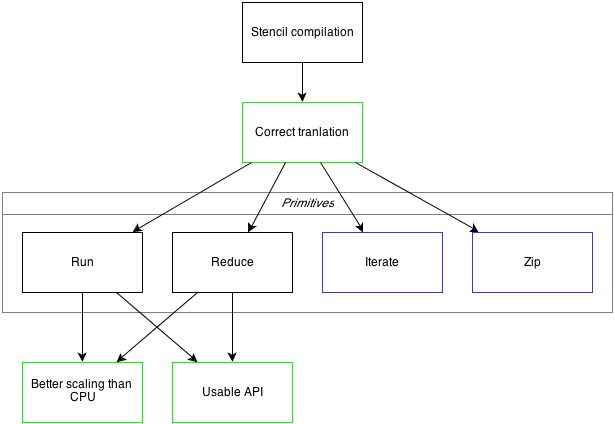
\includegraphics[width=\textwidth ]{figs/ypnos-task-dependency.pdf}
  \caption{This figure depicts the major task dependencies. The black boxes
    represent functional requirements, whereas the green boxes depict
    non-functional ones. Blue boxes are extensions.}
  \label{fig:task-dep}
\end{figure}

\section{Choice of Tools}

In this project I made use of both development tools, such as programming
languages and source control, as well as libraries for software reuse. Below, I
discuss the advantages and disadvantages of the tools, languages, and libraries
chosen

To familiarise myself with Ypnos, Accelerate and other tools, I started with
implementing sample functions in both. The main sample function was an average
stencil (which calculates the mean of its neighbour cell). Example code for this
stencil was given in \autoref{lst:ypsyn1} and will be discussed in detail in
\autoref{sec:introduction-ypnos}.

\subsection{Programming Languages}

Haskell was the obvious choice of programming language, given that Ypnos is
already developed in it. Having not programmed in Haskell before, I had to
become familiar with its more advanced features which were required by my
project (see \autoref{chap:impl}): \emph{type classes}, \emph{type families} and
\emph{data families}.

Haskell has excellent tools for developing compilers: strong typing, pattern
matching and mature parsing libraries
(Parsec\footnote{\url{http://hackage.haskell.org/package/parsec}}).
Furthermore, using the same language as the original implementation allowed for
much code reuse.

\subsection{Development Tools}

To aid the fetching of dependencies and the building of various targets I used
the \emph{Cabal} build system for
Haskell\footnote{\url{http://www.haskell.org/cabal/}}. Cabal features automatic
dependencies resolution and fetching as well as project building tools. By
writing some toy functions to test my knowledge of the Ypnos language I was also
able to set up a test build system in Cabal that I would later use in the rest
of my project. Cabal was chosen as it allowed me to automatically fetch and
install all the dependencies for my project as well as manage their versions and
compatibility.

\emph{Git} version control was used extensively throughout this project for
logging and backup. Although I was already quite familiar with this system, the
project allowed me to make use of some of Git's more advanced features such as
\emph{stashing}, \emph{sub-projects} and \emph{branching}. It was chosen
primarily for these advanced features as well as tight integration with free
hosting services such as \emph{Github}. This allowed my project to be frequently
backed up to the cloud.

\subsection{Libraries}
\subsubsection{Accelerate}

\emph{Accelerate} is a Haskell library which provides GPU accelerated array
computations. It is the only GPU programming library in Haskell which is
sufficiently powerful for my needs.

I chose Accelerate because of the native Haskell support and stencil
operations. It allowed me to abstract away from compiling to low-level C code
and, instead, concentrate on translating to a more abstract and general API.

Accelerate is discussed further in \autoref{sec:intr-axle}.

\subsubsection{CUDA}

\emph{CUDA} is a General Purpose GPU platform for NVidia devices\cite{cuda}. It
is the oldest framework of its kind but has recently been joined by the more
cross-platform OpenCL. The reason I chose CUDA over OpenCL was that the library
support in Haskell had the most stable support for it (though some experimental
support for OpenCL also exists).

As I do not own a machine with a CUDA enabled graphics card, I was using a
remote machine located in the Computer Laboratory. The sample functions allowed
me to set up the machine with the drivers and configuration required in order to
run the Accelerate library.

\section{Software Engineering Techniques}

This section highlights the software engineering approach taken in the
development of this project.

\subsection{Iterative Development}
\label{sec:iterdev}

Given my unfamiliarity with Haskell and GPU programming I followed the
\emph{iterative} model~\cite{cockburn08} to integrate exploration with
development. The end goal is to satisfy the project requirements. This and the
time constraints are the limiting factors of the iterative cycle.

\begin{figure}
  \centering
  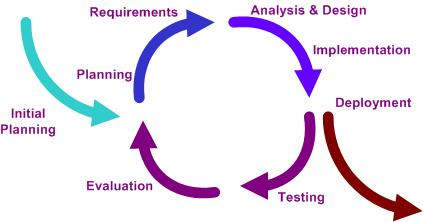
\includegraphics{./figs/Iterative_development_model_V2.jpg}
  \caption{One possible iterative development cycle. In the case of my project
    the deployment stage happened at the deadline and did not include a roll-out
    to actual customers. \\ \emph{Image courtesy of Wikipedia}}
  \label{fig:iterative}
\end{figure}

An iteratively developed project starts with an inception phase in which initial
requirements and goals are layed out. The project then proceeds through cycles
which consist of the following stages (see \autoref{fig:iterative}):

\begin{itemize}
\item
  Gathering requirements
\item
  Design
\item
  Coding
\item
  Testing
\item
  Evaluation
\end{itemize}

The first and last stages in the cycle merge together as requirements for the
next iteration feed off the examination of the last. After each cycle there is
an optional deployment phase in which the product is released. This phase is
omitted from the project.

Throughout the project various solution were attempted in phases and
re-evaluated based on issues found in the last iteration.  Iteration finished
when the requirements were met and the time limit reach.

\subsection{Test-Driven Development}
\label{sec:tdd}

The correctness of my implementation was a central goal. In order to achieve
this I took a test-driven approach to development: while writing the
implementation I was simultaneously writing unit tests for the code.  The
approach allowed me to quickly and effectively find bugs which had not already
been found by the Haskell type system.

\emph{QuickCheck} is the Haskell unit testing library\cite{claessen2011} used
throughout this project. QuickCheck and the testing methodology are discussed in
more detail in \autoref{sec:correctness}.

\section{Introduction to Ypnos}
\label{sec:introduction-ypnos}

Ypnos is an existing language with a fully formed syntax and a partial reference
implementation. Before I could start coding the translation from Ypnos to GPU, I
first had to understand and appreciate the reasoning behind the current choices
in the language and implementation.
\begin{figure}[!h]
\centering
% Define block styles
\tikzstyle{block} = [rectangle, draw,
    text width=6em, text centered, minimum height=4em]
\tikzstyle{ypnos} = [block, fill=blue!20]
\tikzstyle{haskell} = [block, fill=yellow!20]
\tikzstyle{bin} = [block, fill=gray!30]
\tikzstyle{surround} = [block, fill=gray!20]
\tikzstyle{line} = [draw, -latex']

\begin{tikzpicture}[row sep=0.5em]
  % Place nodes
  \def\x{7em}
  \node (9) {};
  \matrix[right=of 9] (1)
  {
    \node (title1) {Phase 1};\\
    \node [ypnos] (ypnos1) {Ypnos syntax}; \\
    \node [haskell] (haskell1) {Haskell code}; \\
    \node [ypnos] (libs) {Ypnos primitives}; \\
  };
  \matrix[right=\x of 1] (2)
  {
    \node (title2) {Phase 2}; \\
    \node [haskell] (haskell2) {Haskell code}; & \\
    \node [ypnos] (libs2) {Ypnos primitives}; & \\
  };
  \matrix[right=\x of 2] (3)
  {
    \node (title3) {Phase 3}; \\
    \node [bin] (bin) {Binary};\\
  };
  \begin{pgfonlayer}{background}
    \node [surround] (hasprim1) [fit = (haskell1) (libs)] {};
    \node [surround] (hasprim2) [fit = (haskell2) (libs2)] {};
    \node [surround] (background1) [fit = (title1) (hasprim1)] {};
    \node [surround] (background2) [fit = (title2) (hasprim2)] {};
    \node [surround] (background3) [fit = (title3) (bin)] {};
    \node [haskell] (hasprim1) [fit = (haskell1) (libs)] {};
    \node [haskell] (hasprim2) [fit = (haskell2) (libs2)] {};
  \end{pgfonlayer}
  % Draw edges
  \path [line] (background1) --
  node [midway, text width=6em, text centered, below] {Compile-time macros}
  (background2);
  \path [line] (background2) --
  node  [midway, below] {Compile} (background3);
\end{tikzpicture}
\caption{The compilation stages of an Ypnos program.\label{fig:comp-stages}}
\end{figure}

Ypnos consists of a library with various primitives used as the building blocks
of programs. Ypnos also provides some custom syntax via macros (see
\autoref{fig:comp-stages}).

\subsection{Grids}

The core data type in Ypnos is the \emph{grid}. As previously mentioned in
\autoref{sec:ypnos}, the grid is Ypnos' generalisation of the array. Unlike
the array, an Ypnos grid is implementation agnostic and could be implemented
differently with different backends.

Ypnos is designed with higher dimensions in mind so the grid may be
multi-dimensional (1D, 2D, etc.). In theory, the variable dimensionality of the
grids allows Ypnos stencil operations to be n-dimensional (although the
implementation doesn't currently support this).

\subsection{Parallelisation}

The stencil as a pattern is particularly good at exposing SIMD parallelism. On
systems like GPUs the amount of data sharing allowed is
restricted\footnote{Access to global shared memory (between thread blocks) is
  expensive. Instead thread block local memory should be used.}, which means
that operations on the different cores must be highly data parallel.

By \emph{subdivision} we are able to split a large grid into many subgrids (see
\autoref{fig:sten-decomp}). The stencils can operate over their subgrids in
parallel because the write-back points of each stencil never overlap. Therefore,
the stencils can safely read from a shared source grid.

\begin{figure}[h]
\centering
\begin{subfigure}{0.45\textwidth}
\centering
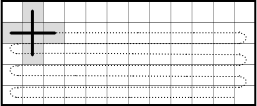
\includegraphics[width=0.95\textwidth]{figs/stencil-diagram.pdf}
\caption{Before subdivision}
\end{subfigure}
~
\begin{subfigure}{0.45\textwidth}
\centering
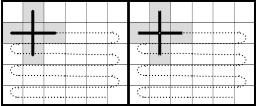
\includegraphics[width=0.95\textwidth]{figs/stencil-parallelised.pdf}
\caption{After subdivision}
\end{subfigure}
\caption{Subdivision of a grid for a 5-point stencil. The cursor location is
  shifted across the whole grid to produce a new grid.}
\label{fig:sten-decomp}
\end{figure}

\subsection{Stencil Syntax}

The Ypnos language provides a custom syntax for defining stencil functions as
well as a collection of primitive operations for their manipulation and use.

The code for a simple two dimensional averaging stencil is shown in
\autoref{lst:ypsyn2}.

\begin{hlisting}[label={lst:ypsyn2},caption={The simple mean function from \autoref{lst:ypsyn1}}]
avg2D :: Grid (Dim X :* Dim Y) a -> a
avg2D = [fun| X*Y:|_  a _|
                  |b @c d|
                  |_  e _| -> (a + b + c + d + e )/5|]
out = run avg2D in -- Running the stencil on `in' to produce `out'
\end{hlisting}

Compare this with the much more verbose imperative version of the same stencil
in \autoref{lst:avgimp}.  The \texttt{fun} macro is used to provide a
special \emph{grid pattern} syntax. The basic syntax of Ypnos can be summarised
as follows:

\begin{tabular}{p{0.1\textwidth} p{0.8\textwidth}}

  \texttt{X*Y:} & The syntax defines the dimensionality of the
  stencil. \texttt{X} and \texttt{Y} are both dimension variables (as is
  \texttt{Z}). They are combined usingthe \texttt{*} operator.  \\

\texttt{|} & The arguments are enclosed within pipe characters.  Their
arrangement in code is typically indented to reflect their grid shape.  \\

\texttt{a,b,\_} & Arguments can either be named or wildcard denoted
respectively with either a variable name or an underscore.  \\

\texttt{@} & This annotation denotes the variable is the cursor, the central cell whose position is used for the
result of the stencil (see \autoref{sec:primitives}).  \\

\texttt{->} & Delimiter that separates the grid pattern and the stencil body. It
appears to be normal Haskell syntax apart from recursion and function
definition.
\\

\end{tabular}

A generic stencil has a type of \texttt{Grid D a -> a} where \texttt{D} is the
dimensionality and \texttt{a} -- the element type. The dimensionality would take
the form \texttt{Dim X :* Dim Y} for a 2D grid.

\begin{hflisting}[label=lst:avgimp, caption={An imperative implementation of the
    average function. Note that the \texttt{in} index values have been laid out in the shape of the grid.}]
double in [M][N]; // Input array
double out [M][N]; // Output array
for (i = 1; i < M-1; i++){
  for (j = 1; j < N-1; j++){
    out[i][j] =
                 (in[i-1][j] +
     in[i][j-1] + in[i][j] + in[i][j+1]
                + in[i+1][j]) / 5;
  }
}
\end{hflisting}

\subsection{Primitives}
\label{sec:primitives}

As well as the syntax for stencil functions, Ypnos provides a library of
primitive operations. The primitives can be combined to create complex
accelerated computations over grids. The main primitive in Ypnos is \emph{run}
(see \autoref{lst:run-red}), which applies the stencil computation to a
grid.

\begin{hflisting}[label={lst:run-red}, caption={The basic \texttt{run},
\texttt{reduce} and, \texttt{reduceR} primitive as defined in the original Ypnos
paper\cite{ypnos-damp10}. \texttt{reduceR} provides a more general version of
the reducer allowing for intermediary values.}]

run :: (Grid D a -> b) -> Grid D a -> Grid D b

reduce :: (a -> a -> a) -> Grid D a -> a

reduceR :: Reducer a b -> Grid D a -> a
mkReducer :: exists b. (a -> b -> b)
                    -> (b -> b -> b)
                    ->  b
                    -> (b -> c)
                    -> Reducer a
\end{hflisting}

The application is done by moving the stencil cursor over each location in the
grid (we saw this illustrated in \autoref{fig:sten-decomp}). The arguments of
the stencil are taken from positions in the grid relative to the cursor. The
value is then computed using the specified computation and put into the same
cursor location in a \emph{new} grid.

In some locations near the edge of the grid there may not be enough neighbours
to satisfy a stencil. In this case Ypnos provides a special syntax for dealing
with these \emph{boundaries}. The implementation of boundaries is beyond the
scope of this project. However, a brief description of their behaviour will aid
the reader's understanding.

For each boundary of the grid, outside of which the stencil may access, a value
is computed by a user defined function. The function may use the current
location index and values from the grid (accessed via a specially bound
variable). A common boundary -- the \emph{mirror} boundary -- works by providing
the closest value inside the grid when an outside access is made. This is the
boundary that I have tacitly assumed to be default in my implementation.

Another vital primitive of the Ypnos language is the \emph{reduce} primitive
whose purpose is to summarise the contents of a grid in one value (see
\autoref{lst:run-red}). It may be used to compute functions such as the mean,
sum or minimum/maximum.

The primitive uses an associative operator (of type \texttt{a -> a -> a}) to
combine all the elements of the grid to one value. A more general version of
this operator, \emph{reduceR}, also exists (see \autoref{lst:run-red}),
which supports an intermediary type (or partial value).

The \emph{Reducer} data type takes the following parameters:

\begin{itemize}
\itemsep1pt\parskip0pt\parsep0pt
\item
  a function reducing an element and a partial value to a partial value,
\item
  a function reducing two partial values,
\item
  a default partial value
\item
  and a conversion from a partial value to the final value.
\end{itemize}

This Reducer is passed into the \emph{reduceR} primitive taking the place of the
associative operator in the reduce primitive. Clearly, reduce can be implemented
in terms of reduceR and so the latter is the more general.

\section{Introduction to Accelerate}
\label{sec:intr-axle}

We have already mentioned Accelerate as one of the implementors of stencil
convolution. In fact, Accelerate is an excellent target for intermediary code
compilation. While the stencil semantics of Accelerate and Ypnos differ in some
respects, the former is powerful enough to represent the latter. Therefore, the
project will target the Accelerate language instead of CUDA.

Accelerate uses the Haskell type system to differentiate between arrays
on the CPU and GPU. It does this by introducing a type encapsulating GPU
operations. There is a further \emph{stratification} of this type into
scalar and array values. Scalar computations may be composed into
array computations.

\subsection{GPU Computation}

For a process on the CPU to execute a CUDA program it must first send
the program and the data to the GPU. When the result is ready it must be copied
back into the main memory of the process concerned. I will call these two
procedure \emph{copy-on} and \emph{copy-off} respectively (see
\autoref{fig:copyonoff}).

\begin{figure}[tb]
  \includegraphics[width=\textwidth]{figs/copyonoff.pdf}
  \caption{An illustration of copy-on and copy-off times.  }
  \label{fig:copyonoff}
\end{figure}

Accelerate represents this difference in the type system. The \texttt{Acc} type
denotes an operation on the GPU. For the purposes of Accelerate, the only
operations allowed on the GPU are those over arrays. As such, \texttt{Array sh
  e} denotes an array of shape \texttt{sh} and element type \texttt{e}.
\texttt{Acc (Array sh e)} denotes the same but in GPU memory and encapsulate an
operation. This means that when such an array is evaluated a CUDA program must
be executed on the GPU.

Arrays are signalled for use on the GPU via the \texttt{use} primitive.  They
are copied-on, executed and copied-off via \texttt{run}. This primitive is
responsible for the run-time compilation and actual data transfer. All other
operations build an abstract syntax tree (AST) to be compiled by the
\texttt{run} primitive. Together \texttt{use} and \texttt{run} form the
constructors and destructors of the \texttt{Acc} data type (see
\autoref{lst:runuse}).

\begin{hflisting}[label={lst:runuse}, caption=The basic constructors and
  destructors for moving arrays too and from the GPU in Accelerate.]
use :: Array sh e -> Acc (Array sh e)
run :: Acc (Array sh e) -> Array sh e
\end{hflisting}

\subsection{Stratified Language}

The main form of operation in Accelerate is over arrays. However, it is often
desirable to build arrays out of multiple scalar values or functions over
scalars. A classic example of this is the map function which transforms an
entire array by a function over the individual values\footnote{In fact, the map
  function is conceptually similar to stencil application. The difference being
  that stencils take into account the neighbourhood of a cell to compute
  the next value whereas map takes only the central value.}(\autoref{lst:map}). For this reason, in addition to the \texttt{Acc} type,
Accelerate also provides the \texttt{Exp} type where the former represents
collective operations and the latter represents scalar computations. The two
types correspond to the two different types of AST built: one for scalar and the
other for array operations.

\begin{hflisting}[label={lst:map}, caption=The type of the \texttt{map}
  operation as defined by Accelerate.]
map :: (Exp a -> Exp b) -> Acc (Array sh a) -> Acc (Array sh b)
\end{hflisting}

Scalar operations do not support any type of iteration or recursion in order to
prevent divergent operation at run-time. However, most other Haskell code is
allowed. This is achieved by the Haskell type class mechanism (for ad-hoc
polymorphism, discussed further in \autoref{sec:typeclasses})-- Accelerate
provides instances of \texttt{Exp a} for most common classes.

For example, to support addition, subtraction and other numerical operations,
Accelerate provides an instance of the type class \texttt{Num}. This means that
operations can be typed as shown in \autoref{lst:num}.

\begin{hlisting}[label={lst:num}, caption=The type of addition overloaded by Accelerate.]
(+) :: Exp a -> Exp a -> Exp a
1 + 2 + 3 :: Exp Integer
\end{hlisting}

\subsection{Stencil Support}

Whilst \texttt{map} for an array applies a scalar function to every element in
an array, Accelerate provides support for running stencil computations via the
\texttt{stencil} function (see \autoref{lst:sten}).

\begin{hflisting}[label={lst:sten}, caption={The type of the stencil application
  function in Accelerate. Including an example instance of the
  \texttt{Stencil} type class. Many others are also possible.}]
stencil :: Stencil sh a sten =>
           (sten -> Exp b) ->
           Boundary a ->
           Acc (Array sh a) ->
           Acc (Array sh b)

instance Stencil DIM2 a ((Exp a, Exp a, Exp a)
                        ,(Exp a, Exp a, Exp a)
                        ,(Exp a, Exp a, Exp a))
\end{hflisting}

The first parameter is a function which represents the stencil. We see that
\texttt{sten}, the type of the stencil argument, takes the form of a tuple grid
of \texttt{Exp a} element type. This allows Accelerate to use Haskell's function
syntax to define stencils.

The second parameter is the type of boundary. In Accelerate, the types of
boundary allowed are fixed as opposed to Ypnos boundaries which can be fully
specified. One of the types allowed is \texttt{Mirror} (see
\autoref{sec:primitives}).

With these two parameters we have defined an operation which performs the
stencil convolution. An example stencil function is given in
\autoref{lst:ypsten}.

\begin{hlisting}[label={lst:ypsten}, caption={The ``average'' stencil defined
  using Accelerate's syntax.}]
avg :: Exp a => Stencil3x3 a -> Exp a
avg (( _, a, _ )
    ,( b, c, d )
    ,( _, e, _ )) = (a + b + c + d + e) / 5

type Stencil3x3 = ((Exp a, Exp a, Exp a)
                  ,(Exp a, Exp a, Exp a)
                  ,(Exp a, Exp a, Exp a))
\end{hlisting}

\section{Summary}

In this section we have seen an analysis of the project's requirements which
allowed me to prioritise the work for the project. Based on the requirements a
choice of tools and libraries was made. An iterative approach to development was
chosen to meet as many of the requirements as possible in the time given.

At the beginning of the project, time was spent on familiarisation with the
tools and libraries as well as the Ypnos language itself. Complex parts of the
Haskell language were investigated and understood (type classes and
families). The Accelerate library, central to the project, was investigated and
``toy'' programs were implemented in both Ypnos and Accelerate.

\chapter{Implementation}
\label{chap:impl}

The work of the implementation can be roughly split into two large chunks: the
compilation of stencils and the implementation of the primitives. In this
project I am aiming for both an accurate and fast translation as well as one
which is easy for the programmer to use.

In this chapter I will highlight the major implementation approaches taken for
the stencil compilation and primitives as well as an example usage of the
system.

\section{Iterative Development}

The iterative development approach was followed throughout the implementation of
this project. \autoref{tbl:iter} describes the phases of development: each
phase consisted of a working code prototype and a small usability evaluation. In
the following sections I will describe each approach taken in more detail.

\begin{table}
\begin{tabular}{l l | p{11cm}}
  \hline
  Phase 1 & Motivation & Create a working translation and run primitive using Accelerate.\\
  & Produced & The non-unifying approach to primitives and compile time approach to stencil translation with centring (\autoref{sec:non-unify-appr} and \autoref{sec:typesysapp}).
  \\
  Phase 2 & Motivation & Reduce the code changes the programmer must perform and unify the CPU and GPU run primitives.\\
  & Produced & The run and reduce primitives using type class parameters (\autoref{lst:redgrid})
  \\
  Phase 3 & Motivation & Make the return type of the reducer more useful to the user.\\
  & Produced & The run and reduce primitives using data families (\autoref{lst:rundatafam}).
  \\
  Phase 4 & Motivation & Remove the need for the programmer to change many constructors when switching.\\
  & Produced & The final approach using a combination of type synonym families and type class parameters (\autoref{sec:final}).\\
  \hline
\end{tabular}
\caption{The phase of iterative development in this project: for each cycle the motivation and work produced is described. \label{tbl:iter}}
\end{table}

\section{Stencil Compilation}

Compilation of stencils was a central task in this project. The abstract Ypnos
syntax is compiled down to Haskell AST to be run. Accelerate's implementation
has overridden much of the Haskell operators required for this translation
stage, so the bulk of the effort went into producing the functions that contain
the stencil computations. These functions take the form of
\autoref{lst:ypsten}

The arguments are formed as tuples of tuples. The rest of the stencil is normal
Haskell code. However, the return type, \texttt{Exp a}, ensures that all the
operations actually use Accelerate's overridden methods to build an AST. The AST
is then translated at run-time into CUDA code.

Ypnos achieves its custom syntax via Haskell's quasiquoting mechanism, a
language feature which allows the library author to provide custom syntax for
domain specific languages\cite{mainland2007}. The programmer must provide a
parser object (refered to as a quasiquoter). The essential function of a
quasiquoter is to provide an abbreviation for entering the AST manually.

Take, for example, the situation in which we want to write an embedded
language to act as a calculator. We have the AST for our
simple calculator in \autoref{lst:calc}.

\begin{hlisting}[label={lst:calc}, caption={A simple calculator defined using an
  AST (\texttt{Expr}) and using a quasiquoter for abbreviated syntax. The definition of
  \texttt{expr} is omitted.}]
data Expr  =  IntExpr Integer
           |  BinopExpr (Integer -> Integer -> Integer) Expr Expr

e1 = BinopExpr (+) (IntExpr 1) (IntExpr 3)
e2 = [expr| 1 + 3 |]
\end{hlisting}

We see that the quasiquoter \texttt{expr} allows us to abbreviate the expression
\texttt{e1} to the more obvious form of \texttt{e2}.

We could sensibly do the translation from Ypnos to Accelerate stencils in one of
two ways: we (a) use Haskell's type system to mask the difference between the
two operations at compile-time or (b) we use run-time compilation to mask the
difference between the implementations. Benefits and drawbacks of both are
presented in the next section.

\subsection{Centring}
\label{sec:centring}

One way in which Accelerate and Ypnos stencils differ is that the former assumes
that the cursor is at the centre of an odd sized grid ($3 \times 5, 5 \times 5$)
whereas the later allows the user to specify the centre. Ypnos stencils can be
translated to Accelerate stencils by padding the stencil passed to Accelerate
such that the cursor is centred.

Take an example: assume a one dimensional stencil with the cursor at an
off-centre location (denoted by \texttt{c}) -- \autoref{fig:cursor}.

\begin{figure}
  \centering
  \begin{subfigure}[t]{0.45\textwidth}
    \includegraphics[width=\textwidth]{figs/align1.pdf}
    \caption{The stencil before centring. Note the even shape ($4\times1$).}
    \label{fig:cursor}
  \end{subfigure}
  ~
  \begin{subfigure}[t]{0.45\textwidth}
    \includegraphics[width=\textwidth]{figs/align2.pdf}
    \caption{The same stencil after centring. Note the shape is now odd
      ($5\times1$)}
    \label{fig:centredcursor}
  \end{subfigure}
  \caption{Where $a$ is the position of the cursor and $b$ -- the length of the
    stencil.  In this diagram $pad_{start}$ represents the offset which needs to
    be applied to the centre, i.e the amount to pad the start of the
    grid. $pad_{end}$ represents the amount to pad the end of the grid. }
\end{figure}

Now we must determine the padding such that the cursor is centred. This is given
by the following two equations:

\[ pad_{start} = max \{a, b-a-1\} - a \]

\[ pad_{end} = max \{a, b-a-1\} - (b - a - 1) \]

This means that after centring we get \autoref{fig:centredcursor}

In order to implement the centring I had to consider both the one and two
dimensional cases.  It would be quite easy to deal with this in two separate
cases, except it must be possible to extend the approach to higher dimensions. I
considered three principle approaches to doing this: using lists as
intermediaries; using arrays as intermediaries; or operating on the grid
patterns directly via type classes.  Before addressing the approaches I will
mention the types in question (see \autoref{lst:gridpattern}).

\begin{hlisting}[label={lst:gridpattern}, caption=The data type which stores
  the grid patterns in Ypnos. Notice that the dimensionality is not exposed in
  the type but hidden.]
data GridPattern = GridPattern1D DimTag [VarP] |
                   GridPattern2D DimTag DimTag [[VarP]]
\end{hlisting}

\texttt{GridPattern} is the type in the Ypnos AST corresponding to the parsed
pattern of arguments. We see that it takes both a 1D and 2D form where the
variables (their type is \texttt{VarP}) are a list and a list of lists
respectively. We may also note that the dimensionality is expressed directly in
the constructor and as such is not present in the type.

The pattern of arguments in Accelerate is expressed as a tuple in the 1D case
and a tuple of tuples in the 2D case. This representation contains no explicit
information about which variables are cursors as we discussed in the previous
section.

\subsubsection{Type Classes}
\label{sec:typeclasses}

Haskell provides both \emph{parametric} and \emph{ad-hoc} polymorphism. The
former is provided by default in function definitions: each function is made to
work over the most general type possible. The latter is provided via the
mechanism of \emph{type classes}.  I required ad-hoc polymorphism in order to
operate differently on patterns of different dimensionalities.

A type class is declared in two parts: interface and instance. An interface has
a number of type parameters (also called indices) and function type
declarations. It is then possible to declare which types are instances of which
class. This is done by providing concrete types for the indices and concrete
definitions for the functions. \autoref{lst:typeclass} gives an example of a
type class declaration and instance.

\begin{hlisting}[label=lst:typeclass, caption={An example type class for
    equality. Showing the declaration and the instance for integers. Where
    \texttt{integerEq} is the implementation of integer equality on the target
    machine.}]
class Eq a where
  (==) :: a -> a -> Bool

instance Eq Integer where
  x == y =  x `integerEq` y

\end{hlisting}

\subsubsection{Type Families}
\label{sec:typefam}

Type families (also known as indexed type families) allow us to apply the same
kind of parameterisation as in type class to the
types\cite{chakravarty05}. Formally, type families are type functions from one
or more types to a single type. As with type classes there are both head
declarations and instances which define the family. The declaration describes
the \emph{``kind''}\footnote{A kind is the type theoretic name for a type for
  types. \texttt{*} denotes the kind of base types in Haskell.} of the family
and defines how many type arguments are taken.

Type families come in two flavours: data families and type synonym families. The
former allows the data type to be declared differently for different indexes,
whereas the latter allows different types to be synonymous.
\autoref{lst:datafam} gives an example of a data family being used to expose
the dimensionality of a pattern. This allows for the use of ad-hoc polymorphism
later on.

\begin{hlisting}[label=lst:datafam, caption=The data family declares tw<
  different constructors for 1D and 2D lists. The dimensionality of the list is
  exposed in the type.]
data family GridPatt :: * -> * -> *
data instance GridPatt (Int) a     = GridPatt1D Int [a]
data instance GridPatt (Int,Int) a = GridPatt2D (Int, Int) [[a]]
\end{hlisting}

Both flavours can be associated with a type class. In this case the index of the
type class must form part of the index of the type family. The interface and
instance declarations of the type family are bound to the corresponding
declarations of the type class. \autoref{lst:assoctypefam} gives an example
of an associated data family for patterns as opposed to it standing alone in
\autoref{lst:datafam}. The usage of type synonym families will be discussed
in detail in \autoref{sec:intr-type-class}.

\begin{hlisting}[label=lst:assoctypefam, caption={The data family from
    \autoref{lst:datafam} has now been associated with the class
    \texttt{GridIx} to provide the function \texttt{size} for various
    dimensionalities.}]
class (Ix i, Num i, ElMax i) => GridIx i where
    data GridPatt :: * -> * -> *
    size :: GridPatt i a -> i

instance GridIx (Int) where
    data GridPatt (Int) a = GridPatt1D Int [a]
    size (GridPatt1D s _) = s
\end{hlisting}

\subsubsection{Intermediate Approaches}

The first approach to centring taken involved first converting from grid
patterns into lists, then balancing these lists, and finally converting them
into the centred tuples needed for the Accelerate functional representation. In
order to do this I would have to define functions for measuring the location of
the cursor, and padding the lists before and after. This approach proved
difficult as lists did not explicitly incorporate their dimensionality in the
type. This made it hard to treat the 1D and 2D cases differently.

The second approach attempted to use existing array code in order to avoid
writing such functions. The hope was that by converting to arrays, rather than
lists, functions for appending and prepending rows and columns would already
exist. However, this was not the case and I would have had to write these
myself. As such, the intermediary array stage was not the best choice.

\subsubsection{Direct Approach}

The third and final approach was to operate directly on the lists extracted from
the \texttt{GridPattern} types. As previously mentioned, to retain
dimensionality information in the type system a type class was required.  I
designed a class \texttt{GridIx} (see \autoref{lst:gridix}) to perform the
basic operations -- \texttt{addBefore}, \texttt{addAfter}, \texttt{find} and
\texttt{size} -- in a dimension-sensitive way while still being polymorphic.

\begin{hlisting}[label={lst:gridix}, caption=The class declaration of
  \texttt{GridIx} showing the main functions defined for the grid manipulation
  and an associated data family.]
class (Ix i, Num i, ElMax i) => GridIx i where
    data GridPatt i :: * -> *
    addBefore :: i -> a -> GridPatt i a -> GridPatt i a
    addAfter :: i -> a -> GridPatt i a -> GridPatt i a
    find :: (a -> Bool) -> GridPatt i a -> i
    size :: GridPatt i a -> i
\end{hlisting}

The associated data type \texttt{GridPatt} would take the type of the particular
dimensionality of list that is appropriate for a given instance. In the case of
the index type \texttt{Int} we would get \texttt{GridPatt Int a = {[}a{]}} and
in the case of \texttt{(Int, Int)} we get \texttt{{[}{[}a{]}{]}}. This approach
allows the algorithms for centring to be described more generally regardless of
the number of dimensions actually involved.

This is the best and most efficient approach in terms of code reuse. This is why
I adopted this approach in the centring used for compile-time stencil
translation (described next).

\subsection{Compile-time Approach to Translation}
\label{sec:typesysapp}

As we saw in the previous section, the types of the Ypnos CPU stencil and the
Accelerate library's stencil differ wildly. \autoref{lst:avgsten} shows the
difference for the \texttt{avg}\footnote{For the sake of simplicity I have
  excluded the type constraints relating to boundaries as these are long
  and complicated.}  stencil.

\begin{hlisting}[label={lst:avgsten}, caption={The average function implemented
    on both the CPU and GPU. Note the difference in types. The constraints are
    simplified.}]
avgCPU :: (Array a, Floating a) => Grid (Dim X :* Dim Y) a ->     a
avgGPU ::      Floating (Exp a) =>            Stencil3x3 a -> Exp a
\end{hlisting}

In the GPU case we see that the type (once expanded) is tuples of tuples of
\texttt{Exp a}. On the other hand, in the Ypnos case we see that arguments take
the form of a grid, which is exactly the same type as the grids it operates on.

The Ypnos grid type is a \emph{comonad}, a functional programming design pattern
arising from Category Theory. The run primitive is an operation of the comonad,
\texttt{cobind} (\autoref{lst:cobind}).

\begin{hflisting}[label={lst:cobind}, caption={The definition of cobind. Let
    \texttt{D} be a grid of a certain dimension and \texttt{a} and \texttt{b} be
    the types of that grid.}]
cobind :: (D a -> b) -> D a -> D b
\end{hflisting}

The type system approach (or compile-time approach) means that Ypnos stencil
syntax is translated directly to a function with Accelerate type
(e.g. \texttt{avgGPU}) by using a different quasiquoter. This was implemented by
me in the \texttt{funGPU} quasiquoter (see \autoref{sec:usage} for usage
examples). Advanced type-system features in Haskell are used to unify the two
types of stencils. The pros and cons of this approach will be discussed in
\autoref{sec:prims}.

Unfortunately, by translating directly to the Accelerate stencil type we lose
the comonadic nature of the type. This is a shame, because this type is both
informative to the programmer (as it is a functional pattern), yet flexible
enough that by changing the instance of \texttt{D} we change the implementation.

The advantage of this method is that all the translation effort is done at
compile-time allowing the running of the stencil to be more efficient.

\subsection{Run-time Approach to Translation}
\label{sec:runtimetrans}

The second approach to the translation of stencils was to keep the types the
same as Ypnos' original implementation.  This is alluring as it allows us to
both expose more information to the user through the program's type and maintain
the theoretic underpinnings of Ypnos -- the comonadic structure. In order to
achieve this, some run-time conversions had to be done.

As already seen, we would like the \texttt{run} primitive to take the
form given in \autoref{lst:run2}

\begin{hflisting}[label={lst:run2}, caption=The comonadic run type. Changing the
  type of \texttt{g} could change the backend used.]
run :: Comonad g => (g a -> b) -> g a -> g b
\end{hflisting}

We have also seen that Accelerate does not accept stencils of this type (see
\autoref{sec:typesysapp}).  To solve this we previously broke the
comonadicity of the operation but we could attempt to preserve it by introducing
an \emph{arrow} data constructor to abstract the differences in type between the
notion of a stencil function\ in Accelerate and Ypnos. This changes the run
function to that seen in \autoref{lst:runarr}.

\begin{hlisting}[label={lst:runarr}, caption=The type run is generalised to
  using the \texttt{arrow} type.]
run :: Comonad g => (g a `arrow` b) -> g a -> g b
\end{hlisting}

The \texttt{arrow} constructor is parametrized on both \texttt{g a} and
\texttt{b}. To build up an instance of \texttt{arrow} we must pass in the
stencil function to a special constructor. The constructor chosen decides the
implementation used.

While previously (\autoref{sec:typesysapp}) we had to use different versions
of the quasiquoter to produce different stencils at compile-time, we now use the
same quasiquoter but convert the function at run-time. We achieve this by taking
advantage of Haskell's polymorphism which allows a function over type \texttt{a}
to specialise to a function of type \texttt{Exp a'}. This generalisation
combined with the arrow data constructor allows our stencil functions to have
the type in \autoref{lst:arrow-sten}

\begin{hlisting}[label={lst:arrow-sten}, caption=Here we see the type the
  stencil must have in Accelerate (\texttt{stencil}) and the type we can
  generalise to using the \texttt{arrow} type (\texttt{stencil'}).]
stencil :: Comonad g => g (Exp a) -> Exp b
stencil' :: Comonad g => g a `arrow` b
\end{hlisting}

Because of the arrow type, \texttt{stencil} and \texttt{stencil'} can now have
the same type.

The type of stencil accepted by Accelerate is still not of the form \texttt{g
  (Exp a) -\textgreater{} Exp b}. A conversion function builds an Accelerate
stencil (call it \emph{stencil A}) at run-time using the stencil encapsulated in
the arrow data type (call it \emph{stencil B}). Stencil A's arguments are used
to build up a grid of type \texttt{g (Exp a)}, then stencil B is used on this
grid to produce the result of type \texttt{Exp b}, finally this is returned as
stencil A's result. So stencil A behaves as a wrapper around stencil B.

While this run-time conversion creates an overhead, it also simplifies the types
significantly. A technique called deforestation may be used to mitigate the
overhead\footnote{Deforestation is also known as ``short cut fusion''. It is
  essentially an optimisation which eliminates intermediate data
  structures.}. Such optimisation is beyond the scope of this project due to
time constraints.

\section{Primitives}
\label{sec:prims}

The primitives are the second core component of the port to GPU. The
implementation of the primitives had two potential approaches: the first was to
re-implement the primitives in a separate module (a non-unifying approach). In
this case, the user would import whichever implementation they required. This
approach had some drawbacks -- for example, it required the user to change much
of their code between implementations.

This led to the second approach of extracting the functionality of the primitive
into a type class. This solution required the use of some complicated type
features in order to make the types unify. This lead to a further three
possibilities: (a) using a type class parameter for unification, (b) associating
a type family and (c) associating a data type.

The resultant approach was a hybrid of these. In this section I will detail all
the approaches taken and at the end of this section I will discuss the
trade-offs which lead to the final approach.

\subsection{Non-unifying Approach}
\label{sec:non-unify-appr}

The run primitive implemented in Phase 1 (see \autoref{tbl:iter}) used the
compile-time implementation of the stencil function
(\autoref{sec:typesysapp}). At the highest level this meant that the function
\texttt{run} had type given in \autoref{lst:runtype}.

\begin{hlisting}[label={lst:runtype}, caption=The type of run required by Accelerate.]
run :: (Stencil sh x sten) => (sten -> Exp y) -> Grid d x -> Grid d y
\end{hlisting}

However, we see that the type variable \texttt{sh} (required by Accelerate) and
\texttt{d} (required by Ypnos) do not unify requiring another constraint to
reconcile the two. Furthermore, constraints need to then be added for the types
of \texttt{x} and \texttt{y} to satisfy Accelerates \texttt{stencil}
function. In the end this type becomes unwieldy -- it is not straight-forward
for the user to write in their code.

Similar problems would have plagued the implementation of the \texttt{reduce}
primitive. However, having first seen the implementation of the \texttt{run}
primitive I decided that a different approach was necessary so this incarnation
of the \texttt{reduce} primitive was never implemented.

\subsection{Introducing Type Classes}
\label{sec:intr-type-class}

In this project I am aiming to make both an accurate and fast translation as
well as one which is easy for the programmer to use.  With the previous approach
we saw how this did not work for two reasons: (a) the run primitive I
implemented was not related (as far as Haskell was concerned) to the original
CPU primitive, and (b) the types of the two primitives differed, which could
cause compilation to fail if they were swapped.

The ideal would be a function which behaves differently under certain program
conditions. The perfect tool for this job is ad-hoc polymorphism which is
provided in Haskell via type classes (see \autoref{lst:avgsten}). The result is
an implementation of the primitive which changes dependent on a particular type
parameter. The obvious parameter in our case is the grid type, that is, have
different grid types for different backends.

We have seen this before: in some of the code examples I have used the notation
``Comonad g'' to refer to a grid which implements the primitives of Ypnos. This
was a type class approach. However, we run into the same problems as with
stencil translation (see \autoref{sec:runtimetrans}), namely the types of
stencil required by Accelerate and Ypnos differ.

\subsubsection{Type Class Parameter}

\begin{hflisting}[label={lst:redgrid}, caption={The \texttt{ReduceGrid} type
class defined with type parameters for each variable: \texttt{a}, \texttt{b} and
\texttt{c}. The \texttt{RunGrid} type class has type parameter \texttt{grid} and
\texttt{sten} where the later is fully determined by the former.}]
class ReduceGrid grid a b c | grid -> a,
                              grid -> b,
                              grid -> c where
    reduceG :: Reducer a b c-> grid -> c

data Reducer a b c where
    Reducer ::   (a -> b -> b)
              -> (b -> b -> b)
              -> b
              -> (b -> c)
              -> Reducer a b c

instance ReduceGrid CPUGrid a b c where
    reduceG = undefined -- Not implemented
instance ReduceGrid GPUGrid (Exp a) (Exp b) (Exp c) where
    reduceG = undefined -- Not implemented

class RunGrid grid sten | grid -> sten where
    runG :: sten -> grid -> grid

instance RunGrid CPUGrid CPUStencil
instance RunGrid GPUGrid GPUStencil
\end{hflisting}

The approach taken in Phase 2 to reconciling the stencil uses Haskell type
classes parametrized by more than one type. This allows us to abstract over
parts of the type that change to give a unified type. As the reduce primitive
was the first to bring about such issues, let's examine how this approach can be
applied to it (see \autoref{lst:redgrid}).

In this approach we are able to have instances for \texttt{Reducer} for the CPU
and GPU based on the grid type yet we also change the types of values accepted
by the functions of the Reducer. These types correspond to different types of
functions (\texttt{Exp a}) which tells Haskell to use Accelerate's overloaded
versions of operators.

We also see that the \texttt{RunGrid} type class is treated in a similar manner:
the type of grid uniquely determines the type of stencil function required. This
is achieved in Haskell using a \emph{functional dependency} (\texttt{grid ->
  sten}) meaning that the \texttt{grid} parameter uniquely determines the
\texttt{sten} parameter\cite{jones2000}. We see this a couple of times in the
given example.

Unlike the \texttt{reduceG} example, Haskell cannot, without help from the
programmer, choose a different quasiquoter (as is required with the static
approach as seen in \autoref{sec:typesysapp}).

\needspace{3\baselineskip}
In theory, this approach should work, however, it brings some usability
problems. Let's further examine the type of the \texttt{reduceG} primitive
when applied to \texttt{GPUGrid}s (see \autoref{lst:redgpu})

\begin{hflisting}[label={lst:redgpu}, caption={The type of the reducer once the
    Accelerate types are applied.}]
Reducer :: (Exp a -> Exp b -> Exp b)
        -> (Exp b -> Exp b -> Exp b)
        -> (Exp b) -- Default value
        -> (Exp b -> Exp c)
        -> Reducer (Exp a) (Exp b) (Exp c)
reduceG :: Reducer (Exp a) (Exp b) (Exp c)
        -> GPUGrid
        -> Exp c -- Return value
\end{hflisting}

Notice that both the return value and default value of the reducer have type
\texttt{Exp}, which is problematic, as \emph{lifting} and
\emph{unlifting}\footnote{Lifting is the process of promoting something of type
  \texttt{a} to type \texttt{Exp a}. Unlifting is the inverse process. Both
  aren't always possible.}  is not easy for the user to do and the wrapped value
is not particularly useful or meaningful once returned to the user. One approach
to changing this would be to introduce type parameters for the functions rather
than the values. However, the approach taken next offers greater flexibility.

\subsubsection{Associated Type Families}
\label{sec:assoctypefam}

We already encountered associated type families in
\autoref{sec:typefam}. Here we will be using type synonym families as
opposed to data families (Phase 4). These allow the unification of the different
function types required (see \autoref{lst:typesynfam} for an example of type
synonyms families unifying different function types).

\begin{hflisting}[label=lst:typesynfam, caption=The type synonym family is used
  as a type function. It is used to work out the element type of a collection.
  Here the \texttt{Fun} family (representing a one-argument function) can take
  two forms depending on the compilation target.]

type family Fun :: * -> * -> * -> *
type instance Fun CPUGrid a b = (a -> b)
type instance Fun GPUGrid a b = (Exp a -> Exp b)

\end{hflisting}

\needspace{7\baselineskip}
The ideal type for the \texttt{Reducer} in the GPU implementation is given in
\autoref{lst:reduceideal}

\begin{hlisting}[label={lst:reduceideal}, caption={The optimal type for the
    reduce primitive under Accelerate.}]
Reducer :: (Exp a -> Exp b -> Exp b)
        -> (Exp b -> Exp b -> Exp b)
        -> b -- Unlifted default
        -> (Exp b -> Exp c)
        -> Reducer a b c

reduceG :: Reducer a b c -> GPUGrid -> c -- Unlifted return
\end{hlisting}

\needspace{14\baselineskip}

This make the default easier to provide and result easier to use. By examining
this we can deduce that there are actually two types of abstract function
involved: 1- and 2-argument functions of \texttt{Exp}s. If we implement these as
two associated type families we get the behaviour required (see
\autoref{lst:redtypefam})

\begin{hlisting}[label={lst:redtypefam}, caption={The application of type
    families to the reduce primitive.}]
Reducer :: Fun2 g a b b
        -> Fun2 g b b b
        -> b
        -> Fun1 g b c
        -> Reducer g a b c

class ReduceGrid g where
    type Fun1 g a b
    type Fun2 g a b c
    reduceG :: Reducer g a b c -> g -> c
\end{hlisting}

Next I wanted to extend this approach to the run primitive. However, with run we
do not simply have a conversion of types, but also conditions on those types
(called constraints in Haskell). It is possible to encode constraints in a type
family method using a Haskell language extension called
\emph{ConstraintKinds}. This allows us to define a type family which has the
\emph{kind} of \texttt{Constraint} instead of the usual \texttt{*} (denoting
type as seen in \autoref{sec:typefam}). An example of the \texttt{RunGrid}
class modified in this way is given in \autoref{lst:constkind}.

\begin{hlisting}[label={lst:constkind}, caption={The application of type
    families to the run primitive.}]
class RunGrid g where
    type ConStencil g a b sten :: Constraint
    type Stencil g a b sten :: *
    run :: ConStencil g a b => (Stencil g a b) -> g x -> g y

instance RunGrid g where
    type ConStencil g a b sten = (Stencil sh a ~ sten, ShapeOf g ~ sh)
    type Stencil g a b sten = sten -> Exp b
\end{hlisting}

As we see, using associated type families is not general because we are exposing
\texttt{sten} -- a type variable which has no relevance to the CPU
implementation. Though it can be safely ignored, it exposes too much of the
underlying type difference which we are coding against and so does not decouple
the two implementations. As we will see in \autoref{sec:final}, this problem
can be mitigated by taking a hybrid approach.

\subsubsection{Associated data families}
\label{sec:assoc-data-fam}

Associated type families make the type of the stencil function explicit again
(Phase 3), as with the type class parameter. To achieve this we can make use of
associated data families (see \autoref{sec:typefam}). These work in much the
same way as type families, but rather than binding a particular synonym to a
class we bind a data type definition.

\autoref{lst:rundatafam} shows the \texttt{RunGrid} type class defined using
data families. We can see that the data family has replaced both the type and
constraint families from \autoref{sec:assoctypefam}.

\begin{hflisting}[label=lst:rundatafam,
caption=RunGrid with associated data family.]
class RunGrid g where
    data Sten g a b :: *
    runG :: Sten g a b -> g a -> g b
\end{hflisting}

This is done with \emph{generalized algebraic data types} (GADTs, another
Haskell type extension) which, amongst other things, allow us to place arbitrary
type constraints on constructors (\autoref{lst:stendatafam}).

\begin{hlisting}[label=lst:stendatafam,
caption={An example of a stencil data type for the GPU. Note the argument it takes is a stencil function (of type \texttt{sten -> Exp b}) where \texttt{sten} has been constrained in the required way.}]
data Sten (Array sh) a b where
        Sten :: (Shape sh, Stencil sh a sten,  -- constraints
                 Elt a, Elt b) =>              -- |
                (sten -> Exp b)
                -> Sten (Array sh) a b
\end{hlisting}

This allows for much cleaner implementation on our part but requires the
programmer to use different data constructors for the different implementations
(CPU versus GPU stencil functions). This is manageable when we are only dealing
with the different stencil types, however, if we add in the different types of
reduction function too, the programmer must make too many code changes.

\subsection{Final implementation}
\label{sec:final}

\begin{hflisting}[label=lst:final, caption={The final signatures of the
  \texttt{RunGrid} and \texttt{ReduceGrid} classes.}]
class RunGrid g arrow | arr -> g where
    type RunCon g arrow x y :: Constraint
    runG :: RunCon g arrow x y =>
            (x `arr` y)
            -> g x -> g y

class ReduceGrid g where
    type ConstFun1 g a b :: Constraint
    type ConstFun2 g a b c :: Constraint
    type Fun1 g a b
    type Fun2 g a b c
    reduceG :: Reducer g a c -> g a -> c
\end{hflisting}

The final implementation was a trade off between approaches. It combines the
type parameter for the \texttt{arrow} type\footnote{This is effectively the same
  as having used an associated data type, except a type synonym could be
  passed.} in the \texttt{RunGrid} class with associated type families for
constraints and generalized functions in the \texttt{ReduceGrid} class (see
\autoref{lst:final}).

The \texttt{RunGrid} class makes use of functional dependencies to ensure that
the \texttt{arrow} constructor the programmer specifies fully determines the
grid implmentation to be used. When using generalised constructors and
destructors (\autoref{sec:usage}) this means that if the programmer is
building their grids from lists then the correct implementation's grid will be
decided based on the \texttt{arrow} type used.

By using a type and not type synonyms for the stencil function I have eliminated
the need to expose a type variable in the declaration for type synonyms (as seen
in \autoref{sec:assoctypefam}). Now this can be neatly encapsulated within a
GADT.

\section{Usage}
\label{sec:usage}

The examples in \autoref{lst:example} are taken directly from the unit tests
for the application. They show the usage of the generalized constructors as well
as the \texttt{run} and \texttt{reduce} primitives. As we can see the user
doesn't have to deal with any of the types we mentioned previously.

\begin{hflisting}[label=lst:example,
caption=Usage of the final system taken from the unit tests.]

-- Take a list of integers and their dimensions and return the sum.
sum :: [Int] -> (Int, Int) -> Int
sum xs (x,y) =  reduceG (mkReducer (+) (+) 0 id) arr
    where arr = fromList (Z :. x :. y) (cycle xs)

-- Run a floating point stencil of any type
runF sten xs (x, y) = gridData (runG sten xs')
    where xs' = listGrid (Dim X :* Dim Y)
                         (0, 0) (x, y)
                         (cycle xs)
                         mirror

-- The average stencil for GPU
avgGPU = [funGPU| X*Y:|a  b c|
                      |d @e f|
                      |g  h i| ->
        (a + b + c + d + e + f + g + h + i)/9|]

-- The average stencil for CPU
avgCPU = [funCPU| X*Y:|a  b c|
                      |d @e f|
                      |g  h i| ->
        (a + b + c + d + e + f + g + h + i)/9|]

-- Run the average function on the GPU
runAvgGPU = runF (GPUArr avgGPU)

-- Run the average function on the CPU
runAvgCPU = runF (CPUArr avgCPU)

\end{hflisting}

\section{Summary}

Recall from \autoref{sec:introduction-ypnos} that Ypnos is a collection of
syntax extensions and a library of primitives. On top of the previous
implementation, this project implemented: changes to the syntax extensions to
allow the generation of GPU stencils (by implementing the \texttt{funGPU}
quasiquoter), library generalisation and API refinement, a re-factoring of CPU
primitives to fit the new API, and a set of new GPU primitives. See
\autoref{fig:files} for a complete summary of the changes introduced by this
project.

This chapter outlined: stencil compilation and the primitive implementation
(reduce and run). Stencil compilation was attempted in a compile-time and
run-time fashion with centring. Moreover, primitives were implemented in a
non-unifying way and then variously unified: type class parameters, associated
types and data families.

The pros and cons of each approach were discussed and at the end of the chapter
I described the final approach chosen. The chapter is rounded off with a brief
usage example for the translation, primitives, constructors and
destructors.

\begin{figure}[p]
\tikzstyle{every node}=[draw=black,thick,anchor=west]
\tikzstyle{created}=[draw=green,fill=green!30]
\tikzstyle{modified}=[draw=yellow,fill=yellow!30]
\begin{tikzpicture}[%
  grow via three points={one child at (0.5,-0.7) and
  two children at (0.5,-0.7) and (0.5,-1.4)},
  edge from parent path={(\tikzparentnode.south) |- (\tikzchildnode.west)}]
  \node {ypnos}
  child { node [created] {ypnos.cabal -- build file}}
  child { node [created] {benchmarks}
    child { node [created] {Benchmark.hs -- benchmark harness}}
    child { node [created] {Makefile}}
    child { node [created] {plot.py -- plotting functions}}
  }
  child [missing] {}
  child [missing] {}
  child [missing] {}
  child { node [] {src}
    child { node [] {Ypnos}
      child { node [modified] {Core -- modified to provide unifying types}
        child { node [] {Boundary.lhs}}
        child { node [modified] {Combinators.lhs}}
        child { node [] {Dimensions.lhs}}
        child { node [modified] {Grid.lhs}}
        child { node [] {Types.lhs}}
      }
      child [missing] {}
      child [missing] {}
      child [missing] {}
      child [missing] {}
      child [missing] {}
      child { node [created] {CUDA/Expr -- the core contribution}
        child { node [created] {Combinators.hs -- primitives}}
        child { node [created] {Fun.hs -- stencil translation}}
      }
      child [missing] {}
      child [missing] {}
      child { node [created] {Examples -- used for testing.}
        child { node [created] {Reductions.hs}}
        child { node [created] {Stencils.hs}}
      }
      child [missing] {}
      child [missing] {}
      child { node [modified] {Expr}
        child { node [] {Boundary.lhs}}
        child { node [] {Expr.lhs}}
        child { node [modified] {Fun.lhs}}
      }
    }
  }
  child [missing] {}
  child [missing] {}
  child [missing] {}
  child [missing] {}
  child [missing] {}
  child [missing] {}
  child [missing] {}
  child [missing] {}
  child [missing] {}
  child [missing] {}
  child [missing] {}
  child [missing] {}
  child [missing] {}
  child [missing] {}
  child [missing] {}
  child [missing] {}
  child [missing] {}
  child { node [created] {testsuite}
    child { node [created] {Test.hs}}
    child { node [created] {Testing/Ypnos/CUDA/Expr -- tests for all functionality implemented}
      child { node [created] {Combinators.hs}}
      child { node [created] {Fun.hs}}
    }
    child [missing] {}
    child [missing] {}
    child { node [created] {UnitTest.hs}}
  };

\end{tikzpicture}
\caption{The file tree of the final Ypnos project showing all work done. White
  files are unchanged from the original implementation. Green files are
  completely new and created by me. Yellow files were modified from the
  original.}
\label{fig:files}
\end{figure}

\chapter{Evaluation}
\label{chap:evaluation}

The main aims of this project were to produce a correct translation and speed up
over the CPU implementation (see \autoref{sec:reqanal}). In order to test
these two goals I have implemented unit tests throughout the course of this
project and implemented an evaluation suite of programs.

This section discusses the performance evaluation and measures taken to ensure a
correct translation. At the end of the chapter I will highlight the usability
evaluation conducted using the method of \emph{cognitive dimensions}.

\section{Performance}

Before the evaluation I postulated that the GPU should provide a speed up over
the CPU due to its capacity for parallel computation. More specifically, I
expected better scaling in the GPU case compared with the CPU.

\subsection{Methodology}

To measure the run-time I used the \emph{Criterion} library\cite{criterion}
which provides functions for:

\begin{itemize}
\itemsep1pt\parskip0pt\parsep0pt
\item Estimating the cost of a single call to the \texttt{clock} function.  The
  function that times the CPU and GPU.
\item Estimating the clock resolution.
\item Running Haskell functions and timing them discounting the above variations
  in order to get a sample of data.
\item Analysing the sample using \emph{bootstrapping}\cite{efron1981} to
  calculate the mean and confidence interval.
\end{itemize}

In my experimental setup I am using a confidence interval of 95\% and a sample
size (for bootstrapping) of 100 and a resample size of 100,000. The result from
Criterion is a mean with a confidence interval of 95\%. I will use these results
to compare the performance of the various functions implemented.

The machine being used for benchmarking was provided by the Computer Laboratory
and remotely hosted, with specifications:

\begin{itemize}
\itemsep1pt\parskip0pt\parsep0pt
\item
  Ubuntu Linux 12.04 64-bit edition
\item
  Quad core Intel Core i5-2400S CPU clocked at 2.50GHz with a 6M cache
\item
  16GB of core memory
\item Nvidia GeForce 9600 GT graphics card featuring 64 G94 cores with a 512 MB
  framebuffer.
\end{itemize}

\subsection{Overhead}

In order to show the speed-up, I must first discount the effects of copying to
and from the GPU\footnote{Though this is an important factor when considering
  CPU versus GPU, it was also a factor I could not control in this
  project. Therefore, I decided to discount it from my measurements.}. This was
done via an \texttt{identity} function implemented in Accelerate. The identity
function works by copying the data from the CPU to the GPU, performing no
operations on the GPU, then copying the data back. This will allow us to have a
base measure of how fast our computations run without overhead.

\subsection{Benchmark suite}

The benchmark suite must test the speed-up of both primitives: \texttt{run} and
\texttt{reduce}. I have implemented a set of representative functions for each
primitive to test speed across a representative set of calculations. These
functions include:

\begin{itemize}
\itemsep1pt\parskip0pt\parsep0pt
\item \textbf{The Average Stencil} (5-point version, \autoref{lst:example}) that
  we have seen in the previous sections. This function is representative of
  convolution style operations which we may wish to perform on the data. It
  operates over floating point numbers which is a common use case for scientific
  computing.
\item \textbf{The Game of Life Stencil} (\autoref{chap:life}) makes use
  of various boolean functions as well as (externally declared) functions used
  to count the number of \emph{true} values in a list.
\item \textbf{The Total Reducer} (\autoref{lst:example}) when normalised gives
  the mean which constitute one of the most common reduction operations over
  grids.
\end{itemize}

\subsection{Results}

\subsubsection{Run}

\begin{figure}[h]
  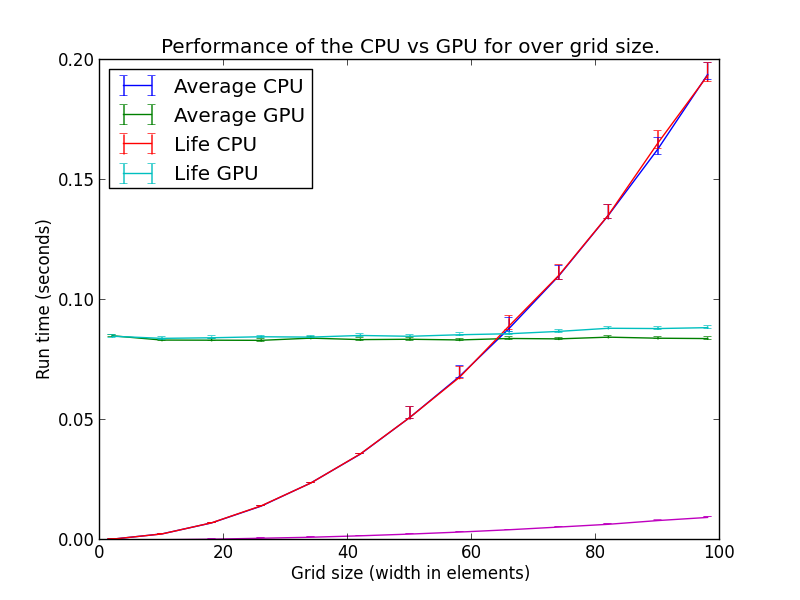
\includegraphics[width=\textwidth]{figs/run_performance.pdf}
  \caption{This plot shows the performance of the CPU versus the GPU
    implementations of the run primitive as it degrades with the grid size
    increasing. The grids are square in shape and the size given is for one of
    its dimensions. For comparison, both the average and game of life stencils
    are depicted. Also shown is the copy-on/off times for the GPU. Error bars
    are shown but most are vanishingly small.}
  \label{fig:runperf100}
\end{figure}

\begin{figure}[h]
  \includegraphics[width=\textwidth]{figs/run_performance2.pdf}
  \caption{This plot shows the performance of the GPU implementations of the run
    primitive as it degrades with a larger scale of grid size. Here we can see
    that both the Game of Life and average function diverge from the base
    measurement. Game of Life degrades the worst due to function calling
    overheads in its implementation. The CPU is not depicted as it grows too
    quickly, dwarfing the GPU measurements. }
  \label{fig:runperf1000}
\end{figure}

\begin{figure}[h]
  \includegraphics[width=\textwidth]{figs/run_performance3.pdf}
  \caption{Here we see the performance of the GPU on the same 0-1000 scale. Now
    the copy on/off time has been discounted by subtraction.}
  \label{fig:runperf1000dis}
\end{figure}

The results of the benchmarking showed that the GPU implementation outperforms
the CPU for grids of size greater than $30 \times 30$. This is in accordance
with the expected outcome, that the GPU is able to perform better modulo copy
on/off times.

On a scale of 0-100 (see \autoref{fig:runperf100}), the slowdown of the GPU
is barely visible above random variation. However, on a greater scale
(\autoref{fig:runperf1000}) it is clear that there is an increase in run
time.

The base measurement is the copy on/off time. We see that on the smaller scale
of analysis the base and actual stencils show little difference in performance
signifying that most of the time is spent in copying (between 20-50\% depending
on the stencil). On the greater scale we see how the stencil computations
actually diverge from the base as GPU computation time starts to become
significant. This can be seen more clearly in \autoref{fig:runperf1000dis}
where the copy on/off time has been discounted.

From the graphs we see that copy on/off time does not account for all the
overhead in the GPU computation. I hypothesise that this is due to a copy on/off
time for code as well as data (which was not accounted for in my
calculations). This is supported by the fact that the Game of Life has a greater
overhead at zero than the average function, because the implementation has
greater code size.

\subsubsection{Reduce}

\begin{figure}[h]
  \includegraphics[width=\textwidth]{figs/reduce_performance.pdf}
  \caption{This plot shows the performance of the CPU versus GPU versions of a
    reduction function. The reduction function given in this case in the sum
    function.}
  \label{fig:reduceperf}
\end{figure}

As we can see from \autoref{fig:reduceperf}, the performance of the reduce
primitive on the GPU also exceeds that of the CPU at $80\times80$ grid
size. This is a consequence of the fact that the reduction calculations are much
less intensive than those of the stencil function or the Game of Life.

\subsection{Deducing a model}

A future goal of this project might be to automatically decide when a certain
workload is best suited to the CPU or GPU. The experiments in this section have
already given us an insight into this: once grid size goes beyond a certain
size, the GPU should be used. We also saw that the complexity of the program
contributes to both the overhead and the scalability. However, at small values
of grid size the overhead of the GPU is most significant and so the degradation
can be ignored.

In order to deduce a model which could be used for switching between CPU and GPU
we must determine (a) an approximation function for the CPU's scalability, which
is mostly dependent on the grid size and (b) the overhead particular to our
program on the GPU, which depends on compiled code size as well as the grid
size. We will ignore (b) seeing as the evaluation was not sufficient to
determine this. (a) can be found by fitting a quadratic to the curve. This has
been done in \autoref{fig:fitting} and we can see that the quadratic
polynomial fits almost perfectly. The coefficients of this polynomial are given
by~\autoref{eq:quad}

\begin{equation} \label{eq:quad}
y = a x^2 + b x + c
\end{equation}
In this equation we can interpret $c$ as being the overhead for the CPU. The
coefficients are:
\begin{align*}
a & = & 3.23223432 \times 10^{-6}\\
b & = & -9.23861372 \times 10^{-6}\\
c & = & 1.56150424 \times 10^{-4}\\
\end{align*}

Knowing the particular overhead of our function, y, (as we have assumed) we are
now able to use \autoref{eq:quad} to calculate the grid size, $x$, for
which we should switch to using the GPU. We set $y$ to the run time of the GPU
operation (which we assumed is constant). Take $y=1.54 \times 10^{-3}$, as is
the case for the average stencil, then we get the resultant switching grid size
$x=22.17$ which agrees with the graph in \autoref{fig:runperf100}.

\begin{figure}[h]
  \includegraphics[width=\textwidth]{figs/run_performance_fit.pdf}
  \caption{Least square error fitting of a linear and quadratic curve to the
    performance data for the CPU implementation of the average function.}
  \label{fig:fitting}
\end{figure}

\section{Correctness}
\label{sec:correctness}

A central goal of the project was to produce a correct translation from Ypnos to
Accelerate. Already, by choosing a type safe language such as Haskell I vastly
reduced the number of run-time errors. To catch the rest I made use of
\emph{unit testing} and \emph{Test Driven Development} (TDD,
\autoref{sec:tdd}). Clearly, unit testing can only provide a partial assurance
of correctness and not a guarantee. However, I decided that a formal proof
(which could give these guarantees) was beyond the scope of this project. In
writing these tests I have assumed that the original CPU implementation was
correct and could be compared against as a gold standard\footnote{However, in
  running my tests I uncovered a bug in the implementation of boundaries which
  had to be fixed before this assumption could hold.}.

The testing framework used works slightly differently to other unit testing
frameworks. In a standard framework the user provides test cases which
incorporate both the test data (sometimes generated) and assertions. In
Haskell's \emph{QuickCheck} we only provide axioms about our functions and let
the framework provide the data based on the type.

Typically, QuickCheck will generate hundreds of test samples to verify a
particular axiom. This provides a better assurance than ordinary unit
testing as, via the random process, QuickCheck often comes up with corner
cases the programmer may not have devised themselves.

The following sections of my project required unit testing:

\begin{itemize}
\item The centring algorithm for grid patterns, as this contains a large part of
  the translations complexity.
\item The \texttt{funGPU} quasiquoter.
\item The \texttt{run} primitive.
\item The \texttt{reduce} primitive.
\end{itemize}

The approach taken to testing the grid patterns was to ensure that the
transformation:

\begin{itemize}
\item
  Starts with a grid that has certain properties (a precondition):
  regular size, positive size, has a cursor.
\item
  Maintains the regularity of size: the length of each row is the same.
\item
  Centres the cursor, given the original grid had a cursor.
\item
  Both roffset and coffset are always positive on such a grid (see
  \autoref{sec:centring} for an explanation of these two values).
\end{itemize}

The assumption was that grid patterns given to the transformation procedures
would be correct to begin with. As such, to improve the amount of test data
generated, I enforced these properties at the generation level. This is safe as
the grid patterns are generated through the CPU translation which I was assuming
to be correct.

To test the primitives I used a standard testing approach of comparing against a
reference implementation. For the \texttt{reduce} primitive I compare against
Haskell's built-in reduce function as I can safely assume this to be
correct. For the \texttt{run} primitive I originally intended to test against
the Ypnos CPU implementation.

The run primitive is tested by running the average function on a randomly
generated grid. The grid is passed to the GPU and CPU implementations of
\texttt{avg}. The resulting grid is then compared between the two and any
difference counts as a failure.

The same procedure is used for the reduce primitive. We use a one-dimensional
grid for this case as the built-in Haskell function we are comparing against is
one-dimensional. The resulting reduced values are compared and a failure is
registered if they should differ.

\section{Usability}

While not mentioned in my original proposal, the usability to the programmer is
another non-functional requirement. This project lacked time for a full
usability study. Instead, evaluated the usability using the method of
\emph{Cognitive Dimensions}~\cite{green96}, to compare the various approaches
already discussed.

Cognitive Dimensions of notations (CD) provide a light-weight vocabulary for
discussing various factors of programming language design. As Ypnos is
essentially a programming language (albeit, one embedded in Haskell) it makes
sense to use this technique. It works by specifying a number of properties of a
notation (\emph{dimensions}, a complete list can be found in
Green\cite{green96}) which must, in general, be traded off against one
another. For this reason it is important to understand the representative tasks
and the user that will be performing them. Then design decisions in the language
can be compared and evaluated using the dimensions relative to the tasks.

\subsection{System = Language + Environment}

It is important to note that CD relates to a whole system, not just the
language. We define the system to be the combination of programming language and
the programming environments. For example, programming over the phone versus
programming in a visual editor. For the purposes of discussing only the language
changes that I have introduced I will fix the environment and assume that it has
the following features:

\begin{itemize}
\item
  Screen-based text editor (e.g.~Vim, Emacs or TextMate)
\item
  Search and replace functionality (including regular expressions)
\end{itemize}

\subsection{Methodology}

I used the following procedure in evaluating the changes to Ypnos using
CD:

\begin{itemize}
\item
  Identify the relevant users of my system and sketch out a basic user
  profile.
\item
  Select the relevant task of these users on the part of the language I
  implemented.
\item
  Highlight which cognitive dimensions are most important to the selected tasks.
\item
  Show a comparison of the various approaches to this implementation.
\item
  Conclude which approach was taken and why.
\end{itemize}

\subsection{User profiles}

I have decided that given the applications to scientific computing and graphics,
the two main types of users would be scientists simulating physical systems and
graphics programmers developing graphics algorithms. I have included two user
stories for our two representative users:

\begin{shadequote}
  Kiaran is a physical scientist who is writing a simulation of a fluid dynamics
  system. He has a little Haskell experience already but has mostly used other
  languages such as Matlab and Fortran. He chose Ypnos/Haskell because he knew
  it would allow him to easily switch between a CPU implementation on his
  machine and a GPU implementation on the simulation machine he is using.
\end{shadequote}

\begin{shadequote}
  Noemi is writing a graphics transformation for a photo editing package. The
  photos her users edit are typically very large but she still would like to
  provide real-time performance with her algorithms. Noemi has a GPU in her
  computer, so she will be writing for this to ensure that her performance is
  good. However, she also wants her system to work on machines that do not have
  a compatible GPU. She already has experience in Haskell and is familiar with
  more complex features and extensions such as type and data families. She has
  picked Ypnos/Haskell because of its syntax and multiple backends.
\end{shadequote}

We can see that there are many tasks that these users would want to
perform with our system: coding up a filter into a stencil (Noemi),
writing a complex reduction to determine the state of the system
(Kiaran), debugging to find out why they get the wrong values (both).
However, I will be ignoring all tasks that involve parts of the system
which I did not implement. This leaves us with one central task for the
two use cases: converting between GPU and CPU.

The cognitive dimensions relevant to this task are:

\begin{tabular}{p{0.35\textwidth} p{0.6\textwidth}}
  Low repetition viscosity & to allow the programmer to easily change the
  implementation without changing too many points in code.
  \\
  Little to no imposed lookahead & allowing the programmer to use one
  implementation without having to think about later switching.
  \\
  Consistency & the programs syntax or usage does not change from CPU to
  GPU, e.g. changing only constructor names.
  \\
  Terseness & the syntax to specify the implementation does not get in the
  way of coding the stencils.
  \\
  Closeness of mapping & the model presented to the programmer through the API
  should map well to their mental model for these types of operation,
  e.g. comonadic operations.
  \\
\end{tabular}

The various approaches to provide an API to the programmer were discussed in the
\autoref{chap:impl}. They essentially boiled down to the following three
approaches: choosing the different implementation based on importing (also
called the non-unifying approach, see \autoref{sec:non-unify-appr}), using
type classes with associated data families (\autoref{sec:assoc-data-fam})
and using type classes with associated type families
(\autoref{sec:assoctypefam} and \autoref{sec:final}). For the sake of
comparison I will also include the approach of the programmer re-coding their
implementation in Accelerate for the GPU.

The results of the evaluation are briefly summarised in
\autoref{tbl:cogcompbrief}, for a full discussion see \autoref{tbl:cogcomp}
in the Appendix. An informal usability analysis such as this one was performed
at the end of each iterative development phase in order to inform the next
prototype.

\begin{longtable}{r | l l l l}
\hline

CD & Accelerate & Non-unifying & Data families & Type families

\\ \hline

Repetition viscosity & \textbf{Worst} & & & \textbf{Best}
\\

Imposed lookahead & \textbf{Worst} & \textbf{Best} & \textbf{Best} &
\textbf{Best}
\\

Consistency & \textbf{Worst} & & & \textbf{Best}
\\

Terseness & \textbf{Worst} & & & \textbf{Best}
\\

Hidden dependencies & \textbf{Best} & \textbf{Worst} & \textbf{Best} &
\textbf{Worst}
\\

Abstraction gradient & \textbf{Best} & & &
\\

Closeness of mapping & \textbf{Best} & \textbf{Worst} & \textbf{Worst} &
\textbf{Worst}
\\
\hline

\caption{A short comparison of the different APIs using cognitive
  dimensions. \label{tbl:cogcompbrief}}
\end{longtable}

\subsection{Discussion of Usability}

As we now can see, the best approach for our users is that of associated type
families with the data constructor for the stencil function. This approach is
best in the viscosity, imposed lookahead, consistency and terseness
dimensions. However, for this it has compromised in hidden dependencies,
abstraction and closeness of mapping.

The \emph{hidden dependency} problems are mitigated by the Haskell compiler
which warns and throws errors when there is a conflict in these dependencies,
e.g. if the user uses different \texttt{Sten} type constructors on the same grid
(see \autoref{lst:stendatafam}). While a little increase in hidden
dependencies is necessary to reduce viscosity, there could be room for
improvement here by making the types more consistent. This would help us remove
the dependencies due to the changing types and constraints.

Given that our example users are fairly advanced, the increase in
\emph{abstraction} should not be a problem, however, we should be aware of this
extra difficulty to learning the language. Advanced features such as type
families are hidden from the users in most cases, so Kiaran should not have a
problem.

The \emph{closeness of mapping} is an issue that is not inherent in the
implementation, but rather an artifact of it. With more time on this
project I would try to re-introduce the comonadic types to the type
family approach. This could require using a lower level implementation
rather than using Accelerate. For this reason getting a closer mapping
was beyond the scope of this project.

\section{Summary}

In this chapter we saw how the performance of my GPU implementation surpasses
that of the CPU for larger grid sizes. This holds for both the run and reduce
primitives. I demonstrated the testing approach taken and discussed how this can
provide some assurance as to the correctness of the translation. Finally, I
conducted usability evaluation using the method of cognitive dimensions.

In summary, this chapter demonstrated all the requirements of the project
(\autoref{sec:reqanal} and original proposal in \autoref{chap:prop}) have been
fulfilled:
\begin{enumerate}
\item Compilation of Ypnos code and implementation of the run primitive on the
  GPU.
\item Implementation of the reduce primitive on the GPU.
\item Better scaling than the current single threaded implementation when
  accounting for copy-on/off times.
\item The translation correctly preserves the semantics of Ypnos.
\end{enumerate}

Furthermore, I have demonstrated the usability of my API, a goal which was not
originally stated.

\chapter{Conclusion}

During this project I have learnt a large number of new and complicated
technologies from a field of computer science previously unknown to me. Having
only experienced the ML functional programming from Part Ia, diving into
Haskell's intricate type system has been an enlightening experience which has
taught me much about my personal software engineering approach and the type
systems of other languages.

\section{Accomplishments}

In this project I have managed to accomplish all the goals laid out by the
original proposal: a correct translation and run primitives which out-perform
their CPU counterparts. Furthermore, I conducted usability evaluation which was
not originally conceived as a requirement.

Aside from the mechanical goals of the project I have also deepened my own
knowledge of computer science and software engineering. I can now add Haskell to
the list of languages I am intimately familiar with. My experience with Haskell
has given me a better understanding of the type theoretic decisions that
underpin other more common languages (such as the various types of polymorphism
used in OOP). Furthermore, my software engineering approaches have been improved
by often needing to re-factor code and design complex systems such as the
centring algorithm.

I consider the project a success in that it both accomplished the requirements
(see \autoref{chap:evaluation}), providing a step forward for the Ypnos
programming language, and helped me learn much about Haskell and GPU
computation.

\section{Lessons Learnt}

In completing this project I have learnt the importance of having a strong plan
to stick to. I realised as I went further into this project that I had not
allocated enough time to researching and learning a new programming
ecosystem. Particularly, I had severely underestimated the time it would take to
get familiar with the complex type theory underlying the Haskell compiler.

Furthermore, if I were to repeat the project I would set out better procedures
for making notes and documenting the project as it progressed. The time required
to compile all the information for the dissertation and understand the different
approaches taken in the implementation was significantly more than I had
previously anticipated. In future work I will endeavour to keep a more complete
diary with frequent reviews of all the work accomplished so far and how it all
fits together.

\section{Future Work}

While all the goals of this project have been achieved, the path of accelerating
Ypnos on the GPU is by no means complete. A number of extensions from the
original proposal still have not been attempted, which include:

\begin{itemize}
\item The \texttt{iterate} primitive which would allow more efficient execution
  of pipelined operations.
\item The \texttt{zip} primitive which would allow implementation of more
  complicated algorithms which require multiple parameters. This would allow
  programs such as \emph{Canny edge detection} to be implemented.
\end{itemize}

Further to the original extensions, during the course of the project more
possible avenues for exploration were discovered. Further exploration may be
possible in:

\begin{itemize}
\item
  Attempting to expose the comonadic nature of operations in the type given to
  the programmer.
\item
  Deducing a full model for the GPU computation overhead.
\item
  Automatic selection of the backend dependent on static program analysis.
\end{itemize}

\printbibliography[heading=bibintoc]

\appendix

\chapter{Original Proposal}
\label{chap:prop}


% Draft #2


% Main document

\bibliographystyle{plain}

\section*{Introduction, The Problem To Be Addressed}

In recent years, Moore's law has begun to plateau. As a result the hardware 
industry has increasingly been turning to MIMD and SIMD architectures as a 
solution.  Some of the highest performing SIMD implementations today are 
provided by GPUs and can be harnessed via GPGPU languages such as CUDA and 
OpenCL.  However, taking advantage of GPGPU is hard as it requires knowledge of 
the low-level concepts of these languages. It is also not portable between 
different hardware and methods of concurrency.

Structured grids are a common computational pattern for scientific parallel 
computation. They allow us to specify \emph{stencils} or \emph{kernels} which 
are local computations that compute a new value from neighboring cells.  
Stencils are promoted to operations over the whole array by application to 
every index.  Many algorithms can be described in this way including the 
Gaussian blur filter, edge detection as well as scientific applications such as 
fluid dynamics. It is also possible to highly parallelize this computation by 
splitting the grid into smaller chunks and running the stencil on each 
separately.

Ypnos \cite{ypnos} is an Embedded Domain Specific Language in the Haskell 
programming language that is capable of describing and running these kernels 
over a grid.  It defines a syntax and various primitives for the structured 
grid computation.  

A kernel is described using a modified Haskell function syntax. The following 
is a kernel used to compute the Gaussian of a grid. The arguments are written 
as a grid and the central point is annotated with \verb|@|. It also denotes the 
location where the kernels return value is written in the new grid.

\begin{verbatim}
ave2D :: Grid (X * Y) Double -> Double
ave2D (X * Y): | _  t _ | = (t+l+c+r+b)/5.0
               | l @c r |
               | _  b _ |
\end{verbatim}

The \emph{run} primitive is used to lift the stencil to a grid operation and 
\emph{iterate} primitive simply recursively applies run. The \emph{reduce} 
primitive allows us to summarise the data so that we can calculate means, sums, 
minimums or maximums. This result is often used as a stopping condition for 
iteration.

The \emph{zip} and \emph{unzip} primitives allow us to pair and unpair the 
values of two grids respectively. This is useful when dealing with multiple 
inter-related quantities as is the case in a physical system with force, 
acceleration and velocity.

Due to the declarative syntax and its purity the order of application of the 
stencils is not important. The author of an Ypnos program does not need to 
worry about the method of concurrency underpinning their program. This allows 
the implementers of Ypnos to use whichever method is most appropriate for the 
given work load and computer. As many computers these days are equipped with 
very advanced GPUs capable of general purpose computation, the Ypnos language 
should be able to use these to accelerate its calculations.

\section*{Starting Point}

\begin{itemize}

\item I have had experience of functional programming from the course as well 
as having completed some Haskell tutorials. 

\item I have experience of building a compiler from Part IB supervision work.

\item During the course of an 11 week internship I learnt to plan, implement, 
document and test my own project.

\item I have already read the Ypnos paper and am familiar with the constructs 
of the language as well its primitives.

\item At present Ypnos has been partially implemented in a single threaded 
fashion on the CPU. The proof-of-concept is only partially implemented. This 
implementation can be taken as both the starting point and the benchmark for 
the new implementation.

\item A Haskell ESDL already exists for compiling array computations to CUDA 
code. The library, ``accelerate'' \cite{accel}, takes an AST and produces code
to run on the GPU.  I will use this library as a back-end to avoid writing a 
compiler to CUDA code directly.

\end{itemize}

\section*{Resources Required}

\begin{itemize} 

\item For this project I shall require my own laptop computer that runs Arch 
Linux for the bulk of development work. 

\item Backup will be to github, the SRCF and/or the MCS. Should my computer 
fail I will be able to use the MCS computers for the project.

\item I require an Nvidia GPU in order to test the code produced. This will be 
provided by Dominic Orchard and I will have access to the machine via SSH for 
testing purposes.

\end{itemize}

\section*{Work to be done}

The project breaks down into the following sub-projects:

\begin{enumerate}

\item Write unit tests that can be used to check the correctness of my 
implementation. The tests will cover micro aspects of the programming language 
such as: constants, unary application, binary application, indexing, 
conditionals, local let-binding, etc.

\item The implementation of the main compilation. This involves writing a 
compilation pass that can take the Ypnos AST and produce a correspondent 
``accelerate'' AST.

\item The implementation of the basic \emph{run} and \emph{reduce} primitives 
as well as any combinators for constructing and deconstructing arrays from raw 
data. The combinators may be written in the ``accelerate'' language directly.

\item The testing of the implementation to check that it works correctly and is 
faster than the original modulo data copying. This will need a test bench to be 
constructed that includes various well know stencil computations. The test 
bench will include the following programs as a minimum: the Game of Life, 
Gaussian blur, Canny edge detection, and (if zip/unzip are implemented) the 
difference of Gaussians.

\end{enumerate}

\section*{Success Criterion for the Main Result}

The project will be a success if:

\begin{enumerate}

\item It can compile Ypnos code and implements the \emph{run} primitive on the 
GPU.

\item It implements the \emph{reduce} primitive on the GPU.

\item It scales better than the current single threaded implementation on large 
work loads. That is to say that when the domain size is increased, the 
difference in computation time increases too. However, this must take into 
account the time required to copy data on and off the GPU.

\item It does all of the above correctly and passes the initial unit tests.

\end{enumerate}

\section*{Possible Extensions}

If the main aim for this project is achieved then I shall try to implement 
further primitives of the Ypnos language. The programmer will then be able to 
take advantage of the speed gains of the GPU pipeline. I will attempt them in 
this order:

\begin{enumerate}

\item The ``iterate'' primitive. This will eliminate the need to copy data 
between the CPU and GPU at each step.

\item The ``zip'' primitive.

\end{enumerate}

I may also attempt to enhance the compiler to decide at compile-time whether to 
use the GPU or CPU dependant on the size of computation required.

\section*{Timetable: Workplan and Milestones to be achieved.}

Planned starting date is 19/10/2011 when the proposal is accepted.

\subsection*{Michaelmas weeks 2-4} Learn to write and read Haskell code. Write 
some programs in Ypnos. Try to understand the existing code base. Start writing 
a unit testing suite.

\subsection*{Michaelmas weeks 5-6} Finish writing the unit testing suite by 
including Gaussian blur and Game of Life programs. Get familiar with the 
``accelerate'' ESDL by reading the paper and writing some toy programs. 

\subsection*{Michaelmas weeks 7-8} Start implementation of the compiler from 
the Ypnos AST to the ``accelerate'' AST. Most basic operations should translate 
correctly by this point.

\subsection*{Michaelmas vacation} Finish the compiler and begin work on 
implementing the run and reduce primitives.

\subsection*{Lent weeks 0-2} Finish the primitives if necessary. Write the 
progress report. Start work on the basic test bench.

\subsection*{Lent weeks 3-5} Finalise the main test bench and run experiments.  
Analyse the performance and scalability of the approach. Make improvements to 
the code as necessary to achieve the main aim of the project. 

\subsection*{Lent weeks 6-8} If there is time then the main extensions may be 
implemented at this point.

\subsection*{Easter vacation} Write the main chapters of the dissertation.

\subsection*{Easter term 0-2} Elaborate on the existing tests bench and run 
final experiments. Complete the dissertation.

\subsection*{Easter term 3} Proof reading and then an early submission.  

\bibliography{refs}


\chapter{Full Cognitive Dimension Analysis}
\label{chap:cogdim}

\newcommand{\sideways}[1]{
  \parbox[t]{2mm}{{\rotatebox[origin=r]{90}{#1}}}}
\newlength{\fstcollen}
\newlength{\sndcollen}
\setlength{\fstcollen}{0.5cm}
\setlength{\sndcollen}{(\textwidth-\fstcollen-2cm)/4}
\begin{longtable}{r | p{\sndcollen} p{\sndcollen} p{\sndcollen} p{\sndcollen}}
\hline\noalign{\medskip}

\sideways{CD}
 &
Accelerate
 &
Non-unifying
 &
Data families
 &
Type families (only stencil data type)

\\\noalign{\medskip}
\hline\noalign{\medskip}

\sideways{Repetition viscosity}
 &
\textbf{Worst}

Clearly here we have a very high viscosity: each function must be re-written in terms of new syntax and run in different ways.
 &
We have improved the viscosity significantly. The user must only
implement their stencils in one language but they must still change all
the imports and correct type errors.
 &
Data families worsen the viscosity over the import method as we must now
change all the data constructors as opposed to the imports. In real code
there will be more of these than import locations.
 &
\textbf{Best}

Here we have the least repetition viscosity of all the approaches. We
now only need to change the quasi quoter to change the whole
implementation.

\\\noalign{\medskip}

\sideways{Imposed lookahead}
 &
\textbf{Worst}

The user must know ahead of time that they will be writing in two
languages to be sure to minimize duplication of code and structure their
program correctly.
 &
\textbf{Best}

There is practially no imposed lookahead as we can simply swap out the
implementation by importing from different places.
 &
\textbf{Best}

We do not have imposed lookahead as we can easily swap the constructors.
 &
\textbf{Best}

There is little imposed lookahead in theory, though some operations are
currently not supported in the GPU implementation. (TODO: link to more)
Some types may not be supported easily in both implementations so this
should be considered too.

\\\noalign{\medskip}

\sideways{Consistency}
 &
\textbf{Worst}

The syntaxes are different and so are fairly inconsistent. There are,
however, some similarities between the two in their stencil
representation.
 &
Consistency is improved as the syntax is now uniform but types are not
uniform.
 &
The syntax and usage is the same except for changing the constructors
which is inconsistent.
 &
\textbf{Best}

We have eliminated the inconsistency in usage of the data families. Now
the approach is almost entirely consistent except for the types.

\\\noalign{\medskip}

\sideways{Terseness}
 &
\textbf{Worst}

A lot of code is written by the user to cope with the two different
implementations.
 &
Changing requires a fair bit of code to be changed as we may be
importing many different things from the Ypnos libraries and all these
things must be changed.
 &
We require a lot of code to express the swap from CPU to GPU.
 &
\textbf{Best}

The syntax for switching is minimally terse.

\\\noalign{\medskip}

\sideways{Hidden dependencies}
 &
\textbf{Best}

No hidden dependencies. It is very clear and explicit what is going on.
 &
\textbf{Worst}

Many hidden dependencies are introduced as the types of the different
imported functions do not necessarily match. This can cause failures in
many different places on changing the import.
 &
\textbf{Best}

Here the dependencies introduced in the type system by the import
approach have been made explicit by data constructors.
 &
\textbf{Worst}

More hidden dependencies are introduced. Types change without the users knowing
due to different type and constraint families. This might affect some programs.

\\\noalign{\medskip}

\sideways{Abstraction gradient}
 &
\textbf{Best}

The abstraction is at its most basic level -- choosing between Ypnos or
Accelerate. The user must get to grips with these abstractions as a
minimum.
 &
The abstraction level is fairly low as it uses only simple Haskell
constructs.
 &
The user must now be familiar with the idea of an associated data family
and GADT which are quite advanced Haskell type features.
 &

The abstraction here is perhaps highest of all as it uses the most
advanced type features.

\\\noalign{\medskip}

\sideways{Closeness of mapping}
 &
\textbf{Best}

This way we preserve the comonadic nature of the operations in the type
so that it is obvious to the user what is going on.
 &
\textbf{Worst}

The comonadicity is lost due to having to change the types to suit the
accelerate implementation.
 &
\textbf{Worst}

The comonadicity is lost also.
 &
\textbf{Worst}

The comonadicity is lost.

\\\noalign{\medskip}
\hline
\noalign{\medskip}
\caption{Comparison of the different API using cognitive dimensions. \label{tbl:cogcomp}}
\end{longtable}


\end{document}
}

\usepackage{fancyheadings}
\pagestyle{fancy}

\title{GPU Accelerating the Ypnos Programming Language}
\author{Samuel Pattuzzi\\ Robinson College}
\date{\today}
%TC:endignore

\begin{document}
\frontmatter

\input{title.tex}

\listoftodos

\chapter{Proforma}

{\large
\begin{tabular}{p{0.3\textwidth} p{0.7\textwidth}}
  Name:               & \bf Samuel Pattuzzi                                 \\
  College:            & \bf Robinson College                                \\
  Project Title:      & \bf \thetitle \\
  Examination:        & \bf Part II Project, June 2013                      \\
  Word Count:         & \bf \wordcount                                      \\
  Project Originator: & D.A. Orchard                                        \\
  Supervisor:         & D.A. Orchard                                        \\
\end{tabular}
}

\section*{Original Aims of the Project}

Creating a backend to the Ypnos programming language to support GPU accelerated
computation. This will require the implementation of translation from the Ypnos
stencil syntax to GPU code. Furthermore, it will require, as a minimum, two
language primitives to be implemented: \emph{run} and \emph{reduce}. Both the
translation and primitives must be correct and, furthermore, outperform the CPU
implementation.

\section*{Work Completed}

The criteria set out in the proposal were met. A backend consisting of a
compilation stage and two primitives was implemented. The correctness of the
implementation was checked by unit testing and benchmarks showed that the
performance of the GPU backend exceeded that of the CPU. In addition, a
usability analysis of the library was performed.

\section*{Special Difficulties}

None.

\newpage
\section*{Declaration}

I, Samuel Pattuzzi of Robinson College, being a candidate for Part II of the
Computer Science Tripos, hereby declare that this dissertation and the work
described in it are my own work, unaided except as may be specified below, and
that the dissertation does not contain material that has already been used to
any substantial extent for a comparable purpose.

I give permission for my dissertation to be made available in the archive
area of the Laboratory's website.

\begin{tabbing}
\bigskip \\
Signed   \= \\
\medskip \\
Date \> \thedate \\
\end{tabbing}

\cleardoublepage
{
 \hypersetup{linkcolor=black}
\setcounter{tocdepth}{2}
\tableofcontents
}
\cleardoublepage


\mainmatter

\chapter{Introduction}

In this project I created a compiler\footnote{We take compiler to mean the
  translation from Ypnos AST to an intermediary and so not the whole compiler
  stack.} for the Ypnos programming language that targets modern GPUs (Graphical
Processing Units) allowing for massive speed-ups of programs in this
language. The language allows programmers to use a very concise syntax to
describe certain types of parallel grid operations. Using this syntax it is now
possible to target machines both with and without compatible GPUs.

\section{Motivation}

GPUs have always been excellent exploiters of SIMD parallelism for graphics
applications. In recent years, however, the GPU pipeline has become more general
than ever. Beyond just providing programmable shaders\footnote{A shader is a
  small program used in graphics applications for simulating lighting effects on
  scenes and objects.} the platform has been opened up, allowing general
programming of GPUs, such as video codec acceleration and even scientific
computing. The ubiquity and low cost of this hardware creates an opportunity for
researchers, professionals and hobbyists alike.

The programming model enforced by the APIs of a GPU can be a significant hurdle
to programming. The APIs of such general purpose GPU (GPGPU) tends to be
low-level but at the same time restricted in ways that may be unfamiliar to the
user. Particularly, memory access within a thread is limited to allow effective
parallelism.

An alternative to using these lowest level APIs is higher level computational
paradigms which expose the SIMD parallelism of a program. Often these paradigms
are not as powerful, but allow for very concise programs within a certain field
of interest. For example, in the field of scientific computing many operations
can be described in terms of matrix operations, so a matrix manipulation library
could expose the SIMD parallelism needed.

The approach taken in the Ypnos programming language is to target a type of
computation common to graphics algorithms and scientific models. By taking a
simple and easy to learn paradigm and combining it with a declarative API, Ypnos
is able to exploit as much SIMD parallelism as needed under the
surface.

Furthermore, Ypnos is back-end agnostic, meaning its programs can easily be
transported from a GPU to a multi-core CPU or even clustered computers. Prior to
this project, Ypnos supported only CPU execution; this project implements a GPU
backend.

\section{Related work}

Ypnos was originally proposed by Orchard et al.\cite{ypnos-damp10}, as a
language embedded within Haskell with a CPU prototype. Haskell supports GPU
computation via the Accelerate library~\cite{acc-damp11}. I will briefly
introduce the reader to both, giving a grounding for the work to come.

\subsection{Ypnos}
\label{sec:ypnos}

\begin{hflisting}[label={lst:ypsyn1},caption={A simple mean function. Computes
    the mean of the neighbourhood of cells.}, float=h]
avg2D :: Grid (Dim X :* Dim Y) a -> a
avg2D = [fun| X*Y:|_  a _|
                  |b @c d|
                  |_  e _| -> (a + b + c + d + e )/5|]
out = run avg2D in -- Running the stencil on `in' to produce `out'
\end{hflisting}

\emph{Stencil computations} are an idiom used in parallel programming.  They
comprise a \emph{kernel} (or \emph{stencil}) which is applied to each element of
an array\footnote{In Ypnos, arrays are known as \emph{grids} to abstract from
  the implementation details.} of data. The kernel computes a new value for an
array location using its old value and the old values of its neighbouring
cells. Convolutions are a well-known example of stencil computation. An example
stencil is given in \autoref{lst:ypsyn1}. A more in depth explanation is given
in \autoref{sec:introduction-ypnos}.

The idiom is particularly useful in the fields of graphical processing and
scientific computing, where some typical applications include Gaussian blur,
Laplacian of Gaussian (an example of differential equation approximation), edge
detection and many other filter based methods. In the scientific domain, they
are used in the simulation of physical systems via fluid, stress or heat
dynamics.

Ypnos is an \emph{embedded domain specific language} (EDSL) for stencil
computations embedded within the Haskell programming
language~\cite{ypnos-damp10, ypnos-dsl11}. This allows Ypnos to share much of
the syntax and implementation of its host language. Haskell is a particularly
good fit for stencil computations as its purity allows the programmer to write
parallel programs without worrying about the interaction and sharing of state.

\subsection{Accelerate}

\emph{Accelerate}~\cite{acc-damp11} is also an EDSL for the Haskell language.
It implements parallel array computations on the GPU. Modern GPUs provide vast
amounts of SIMD parallelism via general purpose interfaces (GPGPU). Accelerate
uses matrix operations to expose SIMD parallelism to the GPU. This model is
easier for a programmer with a mathematical background to understand and exploit
error free.

Accelerate primarily targets GPUs which support NVIDIA's CUDA extension for
GPGPU programming. The library uses algorithmic skeletons for online CUDA code
generation~\cite{cole1989}. It provides operations such as \texttt{map},
\texttt{zip} and \texttt{fold} and implements its own stencil convolution
function.

We will revisit Accelerate in \autoref{sec:intr-axle}.


\chapter{Preparation}

This chapter introduces the subject detail required to understand the subsequent
chapters of the dissertation. This includes a brief introduction to some of
Haskell's more advanced features, the Ypnos programming language and the
Accelerate library.

Furthermore, this chapter discusses some of the foundational planning and design
choices. This includes the analysis of the initial system requirements, choice
of tools, libraries, programming languages, as well as software engineering
methodology.

\section{Requirements Analysis}
\label{sec:reqanal}

\newcommand{\low}{\ding{108}}
\newcommand{\medium}{\low\low}
\newcommand{\high}{\low\medium}

\newcommand{\mc}[1]{\multicolumn{2}{p{8cm}|}{#1}}
\newcommand{\stripe}[1]{\hline\multicolumn{5}{c}{#1}\\\hline}
\newcommand{\tblheaders}[1]{#1\\ \hline}
\newcommand{\tick}{\ding{52}}

\begin{table}[h]
\centering
\caption{Categorization of the main project requirements. The \emph{Ext} column marks requirements which are considered extensions.\label{tbl:reqanal}}
\begin{tabular}{l l|l|l|l|l}
  \tblheaders{\mc{\textbf{Requirements}} & \textbf{Priority} & \textbf{Difficulty} & \textbf{Risk} & \textbf{Ext}}

  \stripe{\textbf{Functional}}

  \mc{Stencil compilation -- compilation of Ypnos stencil syntax to functions runnable on the GPU.} & \high & \high & \medium &  \\

  \mc{Primitive support -- implementation of the primitive functions on the GPU:} & & & \\
  & Run & \high & \medium & \medium &  \\
  & Reduce & \high & \medium & \medium & \\
  & Iterate & \low & \low & \low & \tick \\
  & Zip & \low & \high & \low & \tick \\

  \stripe{\textbf{Non-Functional}}

  \mc{Correct translation -- ensure that the stencil translation is correct.} & \high & \medium & \high & \\

  \mc{Better scaling than CPU -- verify that the GPU implementation outperforms the CPU implementation.} & \high & \medium & \medium & \\

  \mc{Usable API -- ensure that the API presented to the programmer is usable.} & \medium & \medium & \medium & \tick \\

\end{tabular}
\end{table}

Requirements analysis undertaken in the early stages of this project allowed me
to proceed smoothly and identify potential points of failure early. Each major
goal of the project was categorized according to priority, difficulty and risk
(see \autoref{tbl:reqanal}).

The \emph{priority} signifies the importance to the completion of the project:
essential requirements have been marked as high and optional extensions as
low. Other important factors not mentioned in the proposal have also been
included and marked as medium priority. The \emph{difficulty} gave an estimate
of how hard certain requirements would be to achieve and so help provide an
estimate of how much resource should be dedicated. The \emph{risk} embodies the
initial uncertainty about the implementation details. A high risk requirement is
one that could easily take more time than initially foreseen.

The goals were further divided into \emph{functional} and \emph{non-functional}
requirements. Functional requirements specify what had to be implemented and
built during the course of the project. Non-functional requirements specify how
the system should perform and be tested.

An extra requirement was introduced since the proposal, namely a \emph{usable
  API}. Practically, this means that converting between CPU and GPU
implementations of the same program should require minimal code changes.

High risk and high priority requirements needed special attention to prevent the
project from falling behind schedule. In scheduling the tasks, I took a
risk-driven approach: trying to implement the highest risk functional
requirements first and test the highest risk non-functional requirements
early. At the same time, to ensure compilation correctness I took a test-driven
approach to development. I will talk about this in more detail in
\autoref{sec:tdd}.

From the dependency analysis of \autoref{fig:task-dep} a clear ordering to
the tasks is visible. The following order was adopted for the project: stencil
compilation, correctness verification, essential primitives, evaluation,
extensions.

\begin{figure}[h]
  \centering
  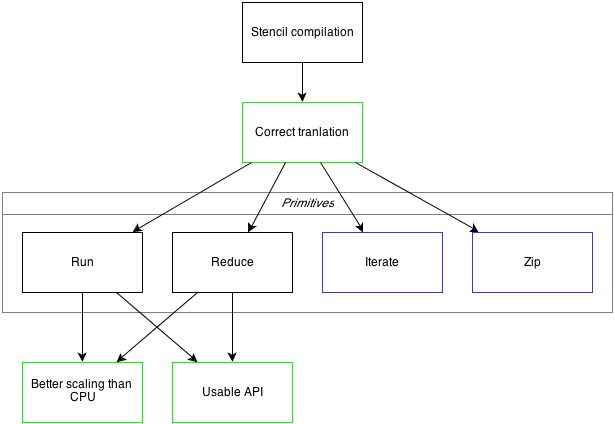
\includegraphics[width=\textwidth ]{figs/ypnos-task-dependency.pdf}
  \caption{This figure depicts the major task dependencies. The black boxes
    represent functional requirements, whereas the green boxes depict
    non-functional ones. Blue boxes are extensions.}
  \label{fig:task-dep}
\end{figure}

\section{Choice of Tools}

In this project I made use of both development tools, such as programming
languages and source control, as well as libraries for software reuse. Below, I
discuss the advantages and disadvantages of the tools, languages, and libraries
chosen

To familiarise myself with Ypnos, Accelerate and other tools, I started with
implementing sample functions in both. The main sample function was an average
stencil (which calculates the mean of its neighbour cell). Example code for this
stencil was given in \autoref{lst:ypsyn1} and will be discussed in detail in
\autoref{sec:introduction-ypnos}.

\subsection{Programming Languages}

Haskell was the obvious choice of programming language, given that Ypnos is
already developed in it. Having not programmed in Haskell before, I had to
become familiar with its more advanced features which were required by my
project (see \autoref{chap:impl}): \emph{type classes}, \emph{type families} and
\emph{data families}.

Haskell has excellent tools for developing compilers: strong typing, pattern
matching and mature parsing libraries
(Parsec\footnote{\url{http://hackage.haskell.org/package/parsec}}).
Furthermore, using the same language as the original implementation allowed for
much code reuse.

\subsection{Development Tools}

To aid the fetching of dependencies and the building of various targets I used
the \emph{Cabal} build system for
Haskell\footnote{\url{http://www.haskell.org/cabal/}}. Cabal features automatic
dependencies resolution and fetching as well as project building tools. By
writing some toy functions to test my knowledge of the Ypnos language I was also
able to set up a test build system in Cabal that I would later use in the rest
of my project. Cabal was chosen as it allowed me to automatically fetch and
install all the dependencies for my project as well as manage their versions and
compatibility.

\emph{Git} version control was used extensively throughout this project for
logging and backup. Although I was already quite familiar with this system, the
project allowed me to make use of some of Git's more advanced features such as
\emph{stashing}, \emph{sub-projects} and \emph{branching}. It was chosen
primarily for these advanced features as well as tight integration with free
hosting services such as \emph{Github}. This allowed my project to be frequently
backed up to the cloud.

\subsection{Libraries}
\subsubsection{Accelerate}

\emph{Accelerate} is a Haskell library which provides GPU accelerated array
computations. It is the only GPU programming library in Haskell which is
sufficiently powerful for my needs.

I chose Accelerate because of the native Haskell support and stencil
operations. It allowed me to abstract away from compiling to low-level C code
and, instead, concentrate on translating to a more abstract and general API.

Accelerate is discussed further in \autoref{sec:intr-axle}.

\subsubsection{CUDA}

\emph{CUDA} is a General Purpose GPU platform for NVidia devices\cite{cuda}. It
is the oldest framework of its kind but has recently been joined by the more
cross-platform OpenCL. The reason I chose CUDA over OpenCL was that the library
support in Haskell had the most stable support for it (though some experimental
support for OpenCL also exists).

As I do not own a machine with a CUDA enabled graphics card, I was using a
remote machine located in the Computer Laboratory. The sample functions allowed
me to set up the machine with the drivers and configuration required in order to
run the Accelerate library.

\section{Software Engineering Techniques}

This section highlights the software engineering approach taken in the
development of this project.

\subsection{Iterative Development}
\label{sec:iterdev}

Given my unfamiliarity with Haskell and GPU programming I followed the
\emph{iterative} model~\cite{cockburn08} to integrate exploration with
development. The end goal is to satisfy the project requirements. This and the
time constraints are the limiting factors of the iterative cycle.

\begin{figure}
  \centering
  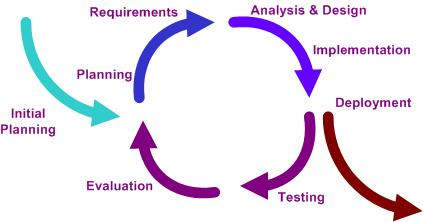
\includegraphics{./figs/Iterative_development_model_V2.jpg}
  \caption{One possible iterative development cycle. In the case of my project
    the deployment stage happened at the deadline and did not include a roll-out
    to actual customers. \\ \emph{Image courtesy of Wikipedia}}
  \label{fig:iterative}
\end{figure}

An iteratively developed project starts with an inception phase in which initial
requirements and goals are layed out. The project then proceeds through cycles
which consist of the following stages (see \autoref{fig:iterative}):

\begin{itemize}
\item
  Gathering requirements
\item
  Design
\item
  Coding
\item
  Testing
\item
  Evaluation
\end{itemize}

The first and last stages in the cycle merge together as requirements for the
next iteration feed off the examination of the last. After each cycle there is
an optional deployment phase in which the product is released. This phase is
omitted from the project.

Throughout the project various solution were attempted in phases and
re-evaluated based on issues found in the last iteration.  Iteration finished
when the requirements were met and the time limit reach.

\subsection{Test-Driven Development}
\label{sec:tdd}

The correctness of my implementation was a central goal. In order to achieve
this I took a test-driven approach to development: while writing the
implementation I was simultaneously writing unit tests for the code.  The
approach allowed me to quickly and effectively find bugs which had not already
been found by the Haskell type system.

\emph{QuickCheck} is the Haskell unit testing library\cite{claessen2011} used
throughout this project. QuickCheck and the testing methodology are discussed in
more detail in \autoref{sec:correctness}.

\section{Introduction to Ypnos}
\label{sec:introduction-ypnos}

Ypnos is an existing language with a fully formed syntax and a partial reference
implementation. Before I could start coding the translation from Ypnos to GPU, I
first had to understand and appreciate the reasoning behind the current choices
in the language and implementation.
\begin{figure}[!h]
\centering
% Define block styles
\tikzstyle{block} = [rectangle, draw,
    text width=6em, text centered, minimum height=4em]
\tikzstyle{ypnos} = [block, fill=blue!20]
\tikzstyle{haskell} = [block, fill=yellow!20]
\tikzstyle{bin} = [block, fill=gray!30]
\tikzstyle{surround} = [block, fill=gray!20]
\tikzstyle{line} = [draw, -latex']
\resizebox {\textwidth} {!} {
\begin{tikzpicture}[row sep=0.5em]
  % Place nodes
  \def\x{7em}
  \matrix[anchor=base west] (1)
  {
    \node (title1) {Phase 1};\\
    \node [ypnos] (ypnos1) {Ypnos syntax}; \\
    \node [haskell] (haskell1) {Haskell code}; \\
    \node [ypnos] (libs) {Ypnos primitives}; \\
  };
  \matrix[right=\x of 1] (2)
  {
    \node (title2) {Phase 2}; \\
    \node [haskell] (haskell2) {Haskell code}; \\
    \node [ypnos] (libs2) {Ypnos primitives}; \\
  };
  \matrix[right=\x of 2] (3)
  {
    \node (title3) {Phase 3}; \\
    \node [bin] (bin) {Binary};\\
  };
  \begin{pgfonlayer}{background}
    \node [surround] (hasprim1) [fit = (haskell1) (libs)] {};
    \node [surround] (hasprim2) [fit = (haskell2) (libs2)] {};
    \node [surround] (background1) [fit = (title1) (hasprim1)] {};
    \node [surround] (background2) [fit = (title2) (hasprim2)] {};
    \node [surround] (background3) [fit = (title3) (bin)] {};
    \node [haskell] (hasprim1) [fit = (haskell1) (libs)] {};
    \node [haskell] (hasprim2) [fit = (haskell2) (libs2)] {};
  \end{pgfonlayer}
  % Draw edges
  \path [line] (background1) --
  node [midway, text width=6em, text centered, below] {Compile-time macros}
  (background2);
  \path [line] (background2) --
  node  [midway, below] {Compile} (background3);
\end{tikzpicture}
}
\caption{The compilation stages of an Ypnos program.\label{fig:comp-stages}}
\end{figure}

Ypnos consists of a library with various primitives used as the building blocks
of programs. Ypnos also provides some custom syntax via macros (see
\autoref{fig:comp-stages}).

\subsection{Grids}

The core data type in Ypnos is the \emph{grid}. As previously mentioned in
\autoref{sec:ypnos}, the grid is Ypnos' generalisation of the array. Unlike
the array, an Ypnos grid is implementation agnostic and could be implemented
differently with different backends.

Ypnos is designed with higher dimensions in mind so the grid may be
multi-dimensional (1D, 2D, etc.). In theory, the variable dimensionality of the
grids allows Ypnos stencil operations to be n-dimensional (although the
implementation doesn't currently support this).

\subsection{Parallelisation}

The stencil as a pattern is particularly good at exposing SIMD parallelism. On
systems like GPUs the amount of data sharing allowed is
restricted\footnote{Access to global shared memory (between thread blocks) is
  expensive. Instead thread block local memory should be used.}, which means
that operations on the different cores must be highly data parallel.

By \emph{subdivision} we are able to split a large grid into many subgrids (see
\autoref{fig:sten-decomp}). The stencils can operate over their subgrids in
parallel because the write-back points of each stencil never overlap. Therefore,
the stencils can safely read from a shared source grid.

\begin{figure}[h]
\centering
\begin{subfigure}{0.45\textwidth}
\centering
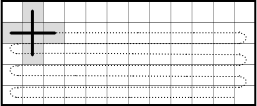
\includegraphics[width=0.95\textwidth]{figs/stencil-diagram.pdf}
\caption{Before subdivision}
\end{subfigure}
~
\begin{subfigure}{0.45\textwidth}
\centering
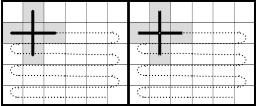
\includegraphics[width=0.95\textwidth]{figs/stencil-parallelised.pdf}
\caption{After subdivision}
\end{subfigure}
\caption{Subdivision of a grid for a 5-point stencil. The cursor location is
  shifted across the whole grid to produce a new grid.}
\label{fig:sten-decomp}
\end{figure}

\subsection{Stencil Syntax}

The Ypnos language provides a custom syntax for defining stencil functions as
well as a collection of primitive operations for their manipulation and use.

The code for a simple two dimensional averaging stencil is shown in
\autoref{lst:ypsyn2}.

\begin{hlisting}[label={lst:ypsyn2},caption={The simple mean function from \autoref{lst:ypsyn1}}]
avg2D :: Grid (Dim X :* Dim Y) a -> a
avg2D = [fun| X*Y:|_  a _|
                  |b @c d|
                  |_  e _| -> (a + b + c + d + e )/5|]
out = run avg2D in -- Running the stencil on `in' to produce `out'
\end{hlisting}

Compare this with the much more verbose imperative version of the same stencil
in \autoref{lst:avgimp}.  The \texttt{fun} macro is used to provide a
special \emph{grid pattern} syntax. The basic syntax of Ypnos can be summarised
as follows:

\begin{tabular}{p{0.1\textwidth} p{0.8\textwidth}}

  \texttt{X*Y:} & The syntax defines the dimensionality of the
  stencil. \texttt{X} and \texttt{Y} are both dimension variables (as is
  \texttt{Z}). They are combined usingthe \texttt{*} operator.  \\

\texttt{|} & The arguments are enclosed within pipe characters.  Their
arrangement in code is typically indented to reflect their grid shape.  \\

\texttt{a,b,\_} & Arguments can either be named or wildcard denoted
respectively with either a variable name or an underscore.  \\

\texttt{@} & This annotation denotes the variable is the cursor, the central cell whose position is used for the
result of the stencil (see \autoref{sec:primitives}).  \\

\texttt{->} & Delimiter that separates the grid pattern and the stencil body. It
appears to be normal Haskell syntax apart from recursion and function
definition.
\\

\end{tabular}

A generic stencil has a type of \texttt{Grid D a -> a} where \texttt{D} is the
dimensionality and \texttt{a} -- the element type. The dimensionality would take
the form \texttt{Dim X :* Dim Y} for a 2D grid.

\begin{hflisting}[label=lst:avgimp, caption={An imperative implementation of the
    average function. Note that the \texttt{in} index values have been laid out in the shape of the grid.}]
double in [M][N]; // Input array
double out [M][N]; // Output array
for (i = 1; i < M-1; i++){
  for (j = 1; j < N-1; j++){
    out[i][j] =
                 (in[i-1][j] +
     in[i][j-1] + in[i][j] + in[i][j+1]
                + in[i+1][j]) / 5;
  }
}
\end{hflisting}

\subsection{Primitives}
\label{sec:primitives}

As well as the syntax for stencil functions, Ypnos provides a library of
primitive operations. The primitives can be combined to create complex
accelerated computations over grids. The main primitive in Ypnos is \emph{run}
(see \autoref{lst:run-red}), which applies the stencil computation to a
grid.

\begin{hflisting}[label={lst:run-red}, caption={The basic \texttt{run},
\texttt{reduce} and, \texttt{reduceR} primitive as defined in the original Ypnos
paper\cite{ypnos-damp10}. \texttt{reduceR} provides a more general version of
the reducer allowing for intermediary values.}]

run :: (Grid D a -> b) -> Grid D a -> Grid D b

reduce :: (a -> a -> a) -> Grid D a -> a

reduceR :: Reducer a b -> Grid D a -> a
mkReducer :: exists b. (a -> b -> b)
                    -> (b -> b -> b)
                    ->  b
                    -> (b -> c)
                    -> Reducer a
\end{hflisting}

The application is done by moving the stencil cursor over each location in the
grid (we saw this illustrated in \autoref{fig:sten-decomp}). The arguments of
the stencil are taken from positions in the grid relative to the cursor. The
value is then computed using the specified computation and put into the same
cursor location in a \emph{new} grid.

In some locations near the edge of the grid there may not be enough neighbours
to satisfy a stencil. In this case Ypnos provides a special syntax for dealing
with these \emph{boundaries}. The implementation of boundaries is beyond the
scope of this project. However, a brief description of their behaviour will aid
the reader's understanding.

For each boundary of the grid, outside of which the stencil may access, a value
is computed by a user defined function. The function may use the current
location index and values from the grid (accessed via a specially bound
variable). A common boundary -- the \emph{mirror} boundary -- works by providing
the closest value inside the grid when an outside access is made. This is the
boundary that I have tacitly assumed to be default in my implementation.

Another vital primitive of the Ypnos language is the \emph{reduce} primitive
whose purpose is to summarise the contents of a grid in one value (see
\autoref{lst:run-red}). It may be used to compute functions such as the mean,
sum or minimum/maximum.

The primitive uses an associative operator (of type \texttt{a -> a -> a}) to
combine all the elements of the grid to one value. A more general version of
this operator, \emph{reduceR}, also exists (see \autoref{lst:run-red}),
which supports an intermediary type (or partial value).

The \emph{Reducer} data type takes the following parameters:

\begin{itemize}
\itemsep1pt\parskip0pt\parsep0pt
\item
  a function reducing an element and a partial value to a partial value,
\item
  a function reducing two partial values,
\item
  a default partial value
\item
  and a conversion from a partial value to the final value.
\end{itemize}

This Reducer is passed into the \emph{reduceR} primitive taking the place of the
associative operator in the reduce primitive. Clearly, reduce can be implemented
in terms of reduceR and so the latter is the more general.

\section{Introduction to Accelerate}
\label{sec:intr-axle}

We have already mentioned Accelerate as one of the implementors of stencil
convolution. In fact, Accelerate is an excellent target for intermediary code
compilation. While the stencil semantics of Accelerate and Ypnos differ in some
respects, the former is powerful enough to represent the latter. Therefore, the
project will target the Accelerate language instead of CUDA.

Accelerate uses the Haskell type system to differentiate between arrays
on the CPU and GPU. It does this by introducing a type encapsulating GPU
operations. There is a further \emph{stratification} of this type into
scalar and array values. Scalar computations may be composed into
array computations.

\subsection{GPU Computation}

For a process on the CPU to execute a CUDA program it must first send
the program and the data to the GPU. When the result is ready it must be copied
back into the main memory of the process concerned. I will call these two
procedure \emph{copy-on} and \emph{copy-off} respectively (see
\autoref{fig:copyonoff}).

\begin{figure}[tb]
  \includegraphics[width=\textwidth]{figs/copyonoff.pdf}
  \caption{An illustration of copy-on and copy-off times.  }
  \label{fig:copyonoff}
\end{figure}

Accelerate represents this difference in the type system. The \texttt{Acc} type
denotes an operation on the GPU. For the purposes of Accelerate, the only
operations allowed on the GPU are those over arrays. As such, \texttt{Array sh
  e} denotes an array of shape \texttt{sh} and element type \texttt{e}.
\texttt{Acc (Array sh e)} denotes the same but in GPU memory and encapsulate an
operation. This means that when such an array is evaluated a CUDA program must
be executed on the GPU.

Arrays are signalled for use on the GPU via the \texttt{use} primitive.  They
are copied-on, executed and copied-off via \texttt{run}. This primitive is
responsible for the run-time compilation and actual data transfer. All other
operations build an abstract syntax tree (AST) to be compiled by the
\texttt{run} primitive. Together \texttt{use} and \texttt{run} form the
constructors and destructors of the \texttt{Acc} data type (see
\autoref{lst:runuse}).

\begin{hflisting}[label={lst:runuse}, caption=The basic constructors and
  destructors for moving arrays too and from the GPU in Accelerate.]
use :: Array sh e -> Acc (Array sh e)
run :: Acc (Array sh e) -> Array sh e
\end{hflisting}

\subsection{Stratified Language}

The main form of operation in Accelerate is over arrays. However, it is often
desirable to build arrays out of multiple scalar values or functions over
scalars. A classic example of this is the map function which transforms an
entire array by a function over the individual values\footnote{In fact, the map
  function is conceptually similar to stencil application. The difference being
  that stencils take into account the neighbourhood of a cell to compute
  the next value whereas map takes only the central value.}(\autoref{lst:map}). For this reason, in addition to the \texttt{Acc} type,
Accelerate also provides the \texttt{Exp} type where the former represents
collective operations and the latter represents scalar computations. The two
types correspond to the two different types of AST built: one for scalar and the
other for array operations.

\begin{hflisting}[label={lst:map}, caption=The type of the \texttt{map}
  operation as defined by Accelerate.]
map :: (Exp a -> Exp b) -> Acc (Array sh a) -> Acc (Array sh b)
\end{hflisting}

Scalar operations do not support any type of iteration or recursion in order to
prevent divergent operation at run-time. However, most other Haskell code is
allowed. This is achieved by the Haskell type class mechanism (for ad-hoc
polymorphism, discussed further in \autoref{sec:typeclasses})-- Accelerate
provides instances of \texttt{Exp a} for most common classes.

For example, to support addition, subtraction and other numerical operations,
Accelerate provides an instance of the type class \texttt{Num}. This means that
operations can be typed as shown in \autoref{lst:num}.

\begin{hlisting}[label={lst:num}, caption=The type of addition overloaded by Accelerate.]
(+) :: Exp a -> Exp a -> Exp a
1 + 2 + 3 :: Exp Integer
\end{hlisting}

\subsection{Stencil Support}

Whilst \texttt{map} for an array applies a scalar function to every element in
an array, Accelerate provides support for running stencil computations via the
\texttt{stencil} function (see \autoref{lst:sten}).

\begin{hflisting}[label={lst:sten}, caption={The type of the stencil application
  function in Accelerate. Including an example instance of the
  \texttt{Stencil} type class. Many others are also possible.}]
stencil :: Stencil sh a sten =>
           (sten -> Exp b) ->
           Boundary a ->
           Acc (Array sh a) ->
           Acc (Array sh b)

instance Stencil DIM2 a ((Exp a, Exp a, Exp a)
                        ,(Exp a, Exp a, Exp a)
                        ,(Exp a, Exp a, Exp a))
\end{hflisting}

The first parameter is a function which represents the stencil. We see that
\texttt{sten}, the type of the stencil argument, takes the form of a tuple grid
of \texttt{Exp a} element type. This allows Accelerate to use Haskell's function
syntax to define stencils.

The second parameter is the type of boundary. In Accelerate, the types of
boundary allowed are fixed as opposed to Ypnos boundaries which can be fully
specified. One of the types allowed is \texttt{Mirror} (see
\autoref{sec:primitives}).

With these two parameters we have defined an operation which performs the
stencil convolution. An example stencil function is given in
\autoref{lst:ypsten}.

\begin{hlisting}[label={lst:ypsten}, caption={The ``average'' stencil defined
  using Accelerate's syntax.}]
avg :: Exp a => Stencil3x3 a -> Exp a
avg (( _, a, _ )
    ,( b, c, d )
    ,( _, e, _ )) = (a + b + c + d + e) / 5

type Stencil3x3 = ((Exp a, Exp a, Exp a)
                  ,(Exp a, Exp a, Exp a)
                  ,(Exp a, Exp a, Exp a))
\end{hlisting}

\section{Summary}

In this section we have seen an analysis of the project's requirements which
allowed me to prioritise the work for the project. Based on the requirements a
choice of tools and libraries was made. An iterative approach to development was
chosen to meet as many of the requirements as possible in the time given.

At the beginning of the project, time was spent on familiarisation with the
tools and libraries as well as the Ypnos language itself. Complex parts of the
Haskell language were investigated and understood (type classes and
families). The Accelerate library, central to the project, was investigated and
``toy'' programs were implemented in both Ypnos and Accelerate.

\chapter{Implementation}
\label{chap:impl}

The work of the implementation can be roughly split into two large chunks: the
compilation of stencils and the implementation of the primitives. In this
project I am aiming for both an accurate and fast translation as well as one
which is easy for the programmer to use.

In this chapter I will highlight the major implementation approaches taken for
the stencil compilation and primitives as well as an example usage of the
system.

\section{Iterative Development}

The iterative development approach was followed throughout the implementation of
this project. \autoref{tbl:iter} describes the phases of development: each
phase consisted of a working code prototype and a small usability evaluation. In
the following sections I will describe each approach taken in more detail.

\begin{table}[h]
\begin{tabularx}{\textwidth}{ll|X}
  \hline
  Phase 1 & Motivation & Create a working translation and run primitive using Accelerate.\\
  & Produced & The non-unifying approach to primitives and compile time approach to stencil translation with centring (\autoref{sec:non-unify-appr} and \autoref{sec:typesysapp}).
  \\
  Phase 2 & Motivation & Reduce the code changes the programmer must perform and unify the CPU and GPU run primitives.\\
  & Produced & The run and reduce primitives using type class parameters (\autoref{lst:redgrid})
  \\
  Phase 3 & Motivation & Make the return type of the reducer more useful to the user.\\
  & Produced & The run and reduce primitives using data families (\autoref{lst:rundatafam}).
  \\
  Phase 4 & Motivation & Remove the need for the programmer to change many constructors when switching.\\
  & Produced & The final approach using a combination of type synonym families and type class parameters (\autoref{sec:final}).\\
  \hline
\end{tabularx}
\caption{The phase of iterative development in this project: for each cycle the motivation and work produced is described. \label{tbl:iter}}
\end{table}

\section{Stencil Compilation}

Compilation of stencils was a central task in this project. The abstract Ypnos
syntax is compiled down to Haskell AST to be run. Accelerate's implementation
has overridden much of the Haskell operators required for this translation
stage, so the bulk of the effort went into producing the functions that contain
the stencil computations. These functions take the form of
\autoref{lst:ypsten}

The arguments are formed as tuples of tuples. The rest of the stencil is normal
Haskell code. However, the return type, \texttt{Exp a}, ensures that all the
operations actually use Accelerate's overridden methods to build an AST. The AST
is then translated at run-time into CUDA code.

Ypnos achieves its custom syntax via Haskell's quasiquoting mechanism, a
language feature which allows the library author to provide custom syntax for
domain specific languages\cite{mainland2007}. The programmer must provide a
parser object (refered to as a quasiquoter). The essential function of a
quasiquoter is to provide an abbreviation for entering the AST manually.

Take, for example, the situation in which we want to write an embedded
language to act as a calculator. We have the AST for our
simple calculator in \autoref{lst:calc}.

\begin{hlisting}[label={lst:calc}, caption={A simple calculator defined using an
  AST (\texttt{Expr}) and using a quasiquoter for abbreviated syntax. The definition of
  \texttt{expr} is omitted.}]
data Expr  =  IntExpr Integer
           |  BinopExpr (Integer -> Integer -> Integer) Expr Expr

e1 = BinopExpr (+) (IntExpr 1) (IntExpr 3)
e2 = [expr| 1 + 3 |]
\end{hlisting}

We see that the quasiquoter \texttt{expr} allows us to abbreviate the expression
\texttt{e1} to the more obvious form of \texttt{e2}.

We could sensibly do the translation from Ypnos to Accelerate stencils in one of
two ways: we (a) use Haskell's type system to mask the difference between the
two operations at compile-time or (b) we use run-time compilation to mask the
difference between the implementations. Benefits and drawbacks of both are
presented in the next section.

\subsection{Centring}
\label{sec:centring}

One way in which Accelerate and Ypnos stencils differ is that the former assumes
that the cursor is at the centre of an odd sized grid ($3 \times 5, 5 \times 5$)
whereas the later allows the user to specify the centre. Ypnos stencils can be
translated to Accelerate stencils by padding the stencil passed to Accelerate
such that the cursor is centred.

Take an example: assume a one dimensional stencil with the cursor at an
off-centre location (denoted by \texttt{c}) -- \autoref{fig:cursor}.

\begin{figure}
  \centering
  \begin{subfigure}[t]{0.45\textwidth}
    \includegraphics[width=\textwidth]{figs/align1.pdf}
    \caption{The stencil before centring. Note the even shape ($4\times1$).}
    \label{fig:cursor}
  \end{subfigure}
  ~
  \begin{subfigure}[t]{0.45\textwidth}
    \includegraphics[width=\textwidth]{figs/align2.pdf}
    \caption{The same stencil after centring. Note the shape is now odd
      ($5\times1$)}
    \label{fig:centredcursor}
  \end{subfigure}
  \caption{Where $a$ is the position of the cursor and $b$ -- the length of the
    stencil.  In this diagram $pad_{start}$ represents the offset which needs to
    be applied to the centre, i.e the amount to pad the start of the
    grid. $pad_{end}$ represents the amount to pad the end of the grid. }
\end{figure}

Now we must determine the padding such that the cursor is centred. This is given
by the following two equations:

\[ pad_{start} = max \{a, b-a-1\} - a \]

\[ pad_{end} = max \{a, b-a-1\} - (b - a - 1) \]

This means that after centring we get \autoref{fig:centredcursor}

In order to implement the centring I had to consider both the one and two
dimensional cases.  It would be quite easy to deal with this in two separate
cases, except it must be possible to extend the approach to higher dimensions. I
considered three principle approaches to doing this: using lists as
intermediaries; using arrays as intermediaries; or operating on the grid
patterns directly via type classes.  Before addressing the approaches I will
mention the types in question (see \autoref{lst:gridpattern}).

\begin{hlisting}[label={lst:gridpattern}, caption=The data type which stores
  the grid patterns in Ypnos. Notice that the dimensionality is not exposed in
  the type but hidden.]
data GridPattern = GridPattern1D DimTag [VarP] |
                   GridPattern2D DimTag DimTag [[VarP]]
\end{hlisting}

\texttt{GridPattern} is the type in the Ypnos AST corresponding to the parsed
pattern of arguments. We see that it takes both a 1D and 2D form where the
variables (their type is \texttt{VarP}) are a list and a list of lists
respectively. We may also note that the dimensionality is expressed directly in
the constructor and as such is not present in the type.

The pattern of arguments in Accelerate is expressed as a tuple in the 1D case
and a tuple of tuples in the 2D case. This representation contains no explicit
information about which variables are cursors as we discussed in the previous
section.

\subsubsection{Type Classes}
\label{sec:typeclasses}

Haskell provides both \emph{parametric} and \emph{ad-hoc} polymorphism. The
former is provided by default in function definitions: each function is made to
work over the most general type possible. The latter is provided via the
mechanism of \emph{type classes}.  I required ad-hoc polymorphism in order to
operate differently on patterns of different dimensionalities.

A type class is declared in two parts: interface and instance. An interface has
a number of type parameters (also called indices) and function type
declarations. It is then possible to declare which types are instances of which
class. This is done by providing concrete types for the indices and concrete
definitions for the functions. \autoref{lst:typeclass} gives an example of a
type class declaration and instance.

\begin{hlisting}[label=lst:typeclass, caption={An example type class for
    equality. Showing the declaration and the instance for integers. Where
    \texttt{integerEq} is the implementation of integer equality on the target
    machine.}]
class Eq a where
  (==) :: a -> a -> Bool

instance Eq Integer where
  x == y =  x `integerEq` y

\end{hlisting}

\subsubsection{Type Families}
\label{sec:typefam}

Type families (also known as indexed type families) allow us to apply the same
kind of parameterisation as in type class to the
types\cite{chakravarty05}. Formally, type families are type functions from one
or more types to a single type. As with type classes there are both head
declarations and instances which define the family. The declaration describes
the \emph{``kind''}\footnote{A kind is the type theoretic name for a type for
  types. \texttt{*} denotes the kind of base types in Haskell.} of the family
and defines how many type arguments are taken.

Type families come in two flavours: data families and type synonym families. The
former allows the data type to be declared differently for different indexes,
whereas the latter allows different types to be synonymous.
\autoref{lst:datafam} gives an example of a data family being used to expose
the dimensionality of a pattern. This allows for the use of ad-hoc polymorphism
later on.

\begin{hlisting}[label=lst:datafam, caption=The data family declares tw<
  different constructors for 1D and 2D lists. The dimensionality of the list is
  exposed in the type.]
data family GridPatt :: * -> * -> *
data instance GridPatt (Int) a     = GridPatt1D Int [a]
data instance GridPatt (Int,Int) a = GridPatt2D (Int, Int) [[a]]
\end{hlisting}

Both flavours can be associated with a type class. In this case the index of the
type class must form part of the index of the type family. The interface and
instance declarations of the type family are bound to the corresponding
declarations of the type class. \autoref{lst:assoctypefam} gives an example
of an associated data family for patterns as opposed to it standing alone in
\autoref{lst:datafam}. The usage of type synonym families will be discussed
in detail in \autoref{sec:intr-type-class}.

\begin{hlisting}[label=lst:assoctypefam, caption={The data family from
    \autoref{lst:datafam} has now been associated with the class
    \texttt{GridIx} to provide the function \texttt{size} for various
    dimensionalities.}]
class (Ix i, Num i, ElMax i) => GridIx i where
    data GridPatt :: * -> * -> *
    size :: GridPatt i a -> i

instance GridIx (Int) where
    data GridPatt (Int) a = GridPatt1D Int [a]
    size (GridPatt1D s _) = s
\end{hlisting}

\subsubsection{Intermediate Approaches}

The first approach to centring taken involved first converting from grid
patterns into lists, then balancing these lists, and finally converting them
into the centred tuples needed for the Accelerate functional representation. In
order to do this I would have to define functions for measuring the location of
the cursor, and padding the lists before and after. This approach proved
difficult as lists did not explicitly incorporate their dimensionality in the
type. This made it hard to treat the 1D and 2D cases differently.

The second approach attempted to use existing array code in order to avoid
writing such functions. The hope was that by converting to arrays, rather than
lists, functions for appending and prepending rows and columns would already
exist. However, this was not the case and I would have had to write these
myself. As such, the intermediary array stage was not the best choice.

\subsubsection{Direct Approach}

The third and final approach was to operate directly on the lists extracted from
the \texttt{GridPattern} types. As previously mentioned, to retain
dimensionality information in the type system a type class was required.  I
designed a class \texttt{GridIx} (see \autoref{lst:gridix}) to perform the
basic operations -- \texttt{addBefore}, \texttt{addAfter}, \texttt{find} and
\texttt{size} -- in a dimension-sensitive way while still being polymorphic.

\begin{hlisting}[label={lst:gridix}, caption=The class declaration of
  \texttt{GridIx} showing the main functions defined for the grid manipulation
  and an associated data family.]
class (Ix i, Num i, ElMax i) => GridIx i where
    data GridPatt i :: * -> *
    addBefore :: i -> a -> GridPatt i a -> GridPatt i a
    addAfter :: i -> a -> GridPatt i a -> GridPatt i a
    find :: (a -> Bool) -> GridPatt i a -> i
    size :: GridPatt i a -> i
\end{hlisting}

The associated data type \texttt{GridPatt} would take the type of the particular
dimensionality of list that is appropriate for a given instance. In the case of
the index type \texttt{Int} we would get \texttt{GridPatt Int a = {[}a{]}} and
in the case of \texttt{(Int, Int)} we get \texttt{{[}{[}a{]}{]}}. This approach
allows the algorithms for centring to be described more generally regardless of
the number of dimensions actually involved.

This is the best and most efficient approach in terms of code reuse. This is why
I adopted this approach in the centring used for compile-time stencil
translation (described next).

\subsection{Compile-time Approach to Translation}
\label{sec:typesysapp}

As we saw in the previous section, the types of the Ypnos CPU stencil and the
Accelerate library's stencil differ wildly. \autoref{lst:avgsten} shows the
difference for the \texttt{avg}\footnote{For the sake of simplicity I have
  excluded the type constraints relating to boundaries as these are long
  and complicated.}  stencil.

\begin{hlisting}[label={lst:avgsten}, caption={The average function implemented
    on both the CPU and GPU. Note the difference in types. The constraints are
    simplified.}]
avgCPU :: (Array a, Floating a) => Grid (Dim X :* Dim Y) a ->     a
avgGPU ::      Floating (Exp a) =>            Stencil3x3 a -> Exp a
\end{hlisting}

In the GPU case we see that the type (once expanded) is tuples of tuples of
\texttt{Exp a}. On the other hand, in the Ypnos case we see that arguments take
the form of a grid, which is exactly the same type as the grids it operates on.

The Ypnos grid type is a \emph{comonad}, a functional programming design pattern
arising from Category Theory. The run primitive is an operation of the comonad,
\texttt{cobind} (\autoref{lst:cobind}).

\begin{hflisting}[label={lst:cobind}, caption={The definition of cobind. Let
    \texttt{D} be a grid of a certain dimension and \texttt{a} and \texttt{b} be
    the types of that grid.}]
cobind :: (D a -> b) -> D a -> D b
\end{hflisting}

The type system approach (or compile-time approach) means that Ypnos stencil
syntax is translated directly to a function with Accelerate type
(e.g. \texttt{avgGPU}) by using a different quasiquoter. This was implemented by
me in the \texttt{funGPU} quasiquoter (see \autoref{sec:usage} for usage
examples). Advanced type-system features in Haskell are used to unify the two
types of stencils. The pros and cons of this approach will be discussed in
\autoref{sec:prims}.

Unfortunately, by translating directly to the Accelerate stencil type we lose
the comonadic nature of the type. This is a shame, because this type is both
informative to the programmer (as it is a functional pattern), yet flexible
enough that by changing the instance of \texttt{D} we change the implementation.

The advantage of this method is that all the translation effort is done at
compile-time allowing the running of the stencil to be more efficient.

\subsection{Run-time Approach to Translation}
\label{sec:runtimetrans}

The second approach to the translation of stencils was to keep the types the
same as Ypnos' original implementation.  This is alluring as it allows us to
both expose more information to the user through the program's type and maintain
the theoretic underpinnings of Ypnos -- the comonadic structure. In order to
achieve this, some run-time conversions had to be done.

As already seen, we would like the \texttt{run} primitive to take the
form given in \autoref{lst:run2}

\begin{hflisting}[label={lst:run2}, caption=The comonadic run type. Changing the
  type of \texttt{g} could change the backend used.]
run :: Comonad g => (g a -> b) -> g a -> g b
\end{hflisting}

We have also seen that Accelerate does not accept stencils of this type (see
\autoref{sec:typesysapp}).  To solve this we previously broke the
comonadicity of the operation but we could attempt to preserve it by introducing
an \emph{arrow} data constructor to abstract the differences in type between the
notion of a stencil function\ in Accelerate and Ypnos. This changes the run
function to that seen in \autoref{lst:runarr}.

\begin{hlisting}[label={lst:runarr}, caption=The type run is generalised to
  using the \texttt{arrow} type.]
run :: Comonad g => (g a `arrow` b) -> g a -> g b
\end{hlisting}

The \texttt{arrow} constructor is parametrized on both \texttt{g a} and
\texttt{b}. To build up an instance of \texttt{arrow} we must pass in the
stencil function to a special constructor. The constructor chosen decides the
implementation used.

While previously (\autoref{sec:typesysapp}) we had to use different versions
of the quasiquoter to produce different stencils at compile-time, we now use the
same quasiquoter but convert the function at run-time. We achieve this by taking
advantage of Haskell's polymorphism which allows a function over type \texttt{a}
to specialise to a function of type \texttt{Exp a'}. This generalisation
combined with the arrow data constructor allows our stencil functions to have
the type in \autoref{lst:arrow-sten}

\begin{hlisting}[label={lst:arrow-sten}, caption=Here we see the type the
  stencil must have in Accelerate (\texttt{stencil}) and the type we can
  generalise to using the \texttt{arrow} type (\texttt{stencil'}).]
stencil :: Comonad g => g (Exp a) -> Exp b
stencil' :: Comonad g => g a `arrow` b
\end{hlisting}

Because of the arrow type, \texttt{stencil} and \texttt{stencil'} can now have
the same type.

The type of stencil accepted by Accelerate is still not of the form \texttt{g
  (Exp a) -\textgreater{} Exp b}. A conversion function builds an Accelerate
stencil (call it \emph{stencil A}) at run-time using the stencil encapsulated in
the arrow data type (call it \emph{stencil B}). Stencil A's arguments are used
to build up a grid of type \texttt{g (Exp a)}, then stencil B is used on this
grid to produce the result of type \texttt{Exp b}, finally this is returned as
stencil A's result. So stencil A behaves as a wrapper around stencil B.

While this run-time conversion creates an overhead, it also simplifies the types
significantly. A technique called deforestation may be used to mitigate the
overhead\footnote{Deforestation is also known as ``short cut fusion''. It is
  essentially an optimisation which eliminates intermediate data
  structures.}. Such optimisation is beyond the scope of this project due to
time constraints.

\section{Primitives}
\label{sec:prims}

The primitives are the second core component of the port to GPU. The
implementation of the primitives had two potential approaches: the first was to
re-implement the primitives in a separate module (a non-unifying approach). In
this case, the user would import whichever implementation they required. This
approach had some drawbacks -- for example, it required the user to change much
of their code between implementations.

This led to the second approach of extracting the functionality of the primitive
into a type class. This solution required the use of some complicated type
features in order to make the types unify. This lead to a further three
possibilities: (a) using a type class parameter for unification, (b) associating
a type family and (c) associating a data type.

The resultant approach was a hybrid of these. In this section I will detail all
the approaches taken and at the end of this section I will discuss the
trade-offs which lead to the final approach.

\subsection{Non-unifying Approach}
\label{sec:non-unify-appr}

The run primitive implemented in Phase 1 (see \autoref{tbl:iter}) used the
compile-time implementation of the stencil function
(\autoref{sec:typesysapp}). At the highest level this meant that the function
\texttt{run} had type given in \autoref{lst:runtype}.

\begin{hlisting}[label={lst:runtype}, caption=The type of run required by Accelerate.]
run :: (Stencil sh x sten) => (sten -> Exp y) -> Grid d x -> Grid d y
\end{hlisting}

However, we see that the type variable \texttt{sh} (required by Accelerate) and
\texttt{d} (required by Ypnos) do not unify requiring another constraint to
reconcile the two. Furthermore, constraints need to then be added for the types
of \texttt{x} and \texttt{y} to satisfy Accelerates \texttt{stencil}
function. In the end this type becomes unwieldy -- it is not straight-forward
for the user to write in their code.

Similar problems would have plagued the implementation of the \texttt{reduce}
primitive. However, having first seen the implementation of the \texttt{run}
primitive I decided that a different approach was necessary so this incarnation
of the \texttt{reduce} primitive was never implemented.

\subsection{Introducing Type Classes}
\label{sec:intr-type-class}

In this project I am aiming to make both an accurate and fast translation as
well as one which is easy for the programmer to use.  With the previous approach
we saw how this did not work for two reasons: (a) the run primitive I
implemented was not related (as far as Haskell was concerned) to the original
CPU primitive, and (b) the types of the two primitives differed, which could
cause compilation to fail if they were swapped.

The ideal would be a function which behaves differently under certain program
conditions. The perfect tool for this job is ad-hoc polymorphism which is
provided in Haskell via type classes (see \autoref{lst:avgsten}). The result is
an implementation of the primitive which changes dependent on a particular type
parameter. The obvious parameter in our case is the grid type, that is, have
different grid types for different backends.

We have seen this before: in some of the code examples I have used the notation
``Comonad g'' to refer to a grid which implements the primitives of Ypnos. This
was a type class approach. However, we run into the same problems as with
stencil translation (see \autoref{sec:runtimetrans}), namely the types of
stencil required by Accelerate and Ypnos differ.

\subsubsection{Type Class Parameter}

\begin{hflisting}[label={lst:redgrid}, caption={The \texttt{ReduceGrid} type
class defined with type parameters for each variable: \texttt{a}, \texttt{b} and
\texttt{c}. The \texttt{RunGrid} type class has type parameter \texttt{grid} and
\texttt{sten} where the later is fully determined by the former.}]
class ReduceGrid grid a b c | grid -> a,
                              grid -> b,
                              grid -> c where
    reduceG :: Reducer a b c-> grid -> c

data Reducer a b c where
    Reducer ::   (a -> b -> b)
              -> (b -> b -> b)
              -> b
              -> (b -> c)
              -> Reducer a b c

instance ReduceGrid CPUGrid a b c where
    reduceG = undefined -- Not implemented
instance ReduceGrid GPUGrid (Exp a) (Exp b) (Exp c) where
    reduceG = undefined -- Not implemented

class RunGrid grid sten | grid -> sten where
    runG :: sten -> grid -> grid

instance RunGrid CPUGrid CPUStencil
instance RunGrid GPUGrid GPUStencil
\end{hflisting}

The approach taken in Phase 2 to reconciling the stencil uses Haskell type
classes parametrized by more than one type. This allows us to abstract over
parts of the type that change to give a unified type. As the reduce primitive
was the first to bring about such issues, let's examine how this approach can be
applied to it (see \autoref{lst:redgrid}).

In this approach we are able to have instances for \texttt{Reducer} for the CPU
and GPU based on the grid type yet we also change the types of values accepted
by the functions of the Reducer. These types correspond to different types of
functions (\texttt{Exp a}) which tells Haskell to use Accelerate's overloaded
versions of operators.

We also see that the \texttt{RunGrid} type class is treated in a similar manner:
the type of grid uniquely determines the type of stencil function required. This
is achieved in Haskell using a \emph{functional dependency} (\texttt{grid ->
  sten}) meaning that the \texttt{grid} parameter uniquely determines the
\texttt{sten} parameter\cite{jones2000}. We see this a couple of times in the
given example.

Unlike the \texttt{reduceG} example, Haskell cannot, without help from the
programmer, choose a different quasiquoter (as is required with the static
approach as seen in \autoref{sec:typesysapp}).

\needspace{3\baselineskip}
In theory, this approach should work, however, it brings some usability
problems. Let's further examine the type of the \texttt{reduceG} primitive
when applied to \texttt{GPUGrid}s (see \autoref{lst:redgpu})

\begin{hflisting}[label={lst:redgpu}, caption={The type of the reducer once the
    Accelerate types are applied.}]
Reducer :: (Exp a -> Exp b -> Exp b)
        -> (Exp b -> Exp b -> Exp b)
        -> (Exp b) -- Default value
        -> (Exp b -> Exp c)
        -> Reducer (Exp a) (Exp b) (Exp c)
reduceG :: Reducer (Exp a) (Exp b) (Exp c)
        -> GPUGrid
        -> Exp c -- Return value
\end{hflisting}

Notice that both the return value and default value of the reducer have type
\texttt{Exp}, which is problematic, as \emph{lifting} and
\emph{unlifting}\footnote{Lifting is the process of promoting something of type
  \texttt{a} to type \texttt{Exp a}. Unlifting is the inverse process. Both
  aren't always possible.}  is not easy for the user to do and the wrapped value
is not particularly useful or meaningful once returned to the user. One approach
to changing this would be to introduce type parameters for the functions rather
than the values. However, the approach taken next offers greater flexibility.

\subsubsection{Associated Type Families}
\label{sec:assoctypefam}

We already encountered associated type families in
\autoref{sec:typefam}. Here we will be using type synonym families as
opposed to data families (Phase 4). These allow the unification of the different
function types required (see \autoref{lst:typesynfam} for an example of type
synonyms families unifying different function types).

\begin{hflisting}[label=lst:typesynfam, caption=The type synonym family is used
  as a type function. It is used to work out the element type of a collection.
  Here the \texttt{Fun} family (representing a one-argument function) can take
  two forms depending on the compilation target.]

type family Fun :: * -> * -> * -> *
type instance Fun CPUGrid a b = (a -> b)
type instance Fun GPUGrid a b = (Exp a -> Exp b)

\end{hflisting}

\needspace{7\baselineskip}
The ideal type for the \texttt{Reducer} in the GPU implementation is given in
\autoref{lst:reduceideal}

\begin{hlisting}[label={lst:reduceideal}, caption={The optimal type for the
    reduce primitive under Accelerate.}]
Reducer :: (Exp a -> Exp b -> Exp b)
        -> (Exp b -> Exp b -> Exp b)
        -> b -- Unlifted default
        -> (Exp b -> Exp c)
        -> Reducer a b c

reduceG :: Reducer a b c -> GPUGrid -> c -- Unlifted return
\end{hlisting}

\needspace{14\baselineskip}

This make the default easier to provide and result easier to use. By examining
this we can deduce that there are actually two types of abstract function
involved: 1- and 2-argument functions of \texttt{Exp}s. If we implement these as
two associated type families we get the behaviour required (see
\autoref{lst:redtypefam})

\begin{hlisting}[label={lst:redtypefam}, caption={The application of type
    families to the reduce primitive.}]
Reducer :: Fun2 g a b b
        -> Fun2 g b b b
        -> b
        -> Fun1 g b c
        -> Reducer g a b c

class ReduceGrid g where
    type Fun1 g a b
    type Fun2 g a b c
    reduceG :: Reducer g a b c -> g -> c
\end{hlisting}

Next I wanted to extend this approach to the run primitive. However, with run we
do not simply have a conversion of types, but also conditions on those types
(called constraints in Haskell). It is possible to encode constraints in a type
family method using a Haskell language extension called
\emph{ConstraintKinds}. This allows us to define a type family which has the
\emph{kind} of \texttt{Constraint} instead of the usual \texttt{*} (denoting
type as seen in \autoref{sec:typefam}). An example of the \texttt{RunGrid}
class modified in this way is given in \autoref{lst:constkind}.

\begin{hlisting}[label={lst:constkind}, caption={The application of type
    families to the run primitive.}]
class RunGrid g where
    type ConStencil g a b sten :: Constraint
    type Stencil g a b sten :: *
    run :: ConStencil g a b => (Stencil g a b) -> g x -> g y

instance RunGrid g where
    type ConStencil g a b sten = (Stencil sh a ~ sten, ShapeOf g ~ sh)
    type Stencil g a b sten = sten -> Exp b
\end{hlisting}

As we see, using associated type families is not general because we are exposing
\texttt{sten} -- a type variable which has no relevance to the CPU
implementation. Though it can be safely ignored, it exposes too much of the
underlying type difference which we are coding against and so does not decouple
the two implementations. As we will see in \autoref{sec:final}, this problem
can be mitigated by taking a hybrid approach.

\subsubsection{Associated data families}
\label{sec:assoc-data-fam}

Associated type families make the type of the stencil function explicit again
(Phase 3), as with the type class parameter. To achieve this we can make use of
associated data families (see \autoref{sec:typefam}). These work in much the
same way as type families, but rather than binding a particular synonym to a
class we bind a data type definition.

\autoref{lst:rundatafam} shows the \texttt{RunGrid} type class defined using
data families. We can see that the data family has replaced both the type and
constraint families from \autoref{sec:assoctypefam}.

\begin{hflisting}[label=lst:rundatafam,
caption=RunGrid with associated data family.]
class RunGrid g where
    data Sten g a b :: *
    runG :: Sten g a b -> g a -> g b
\end{hflisting}

This is done with \emph{generalized algebraic data types} (GADTs, another
Haskell type extension) which, amongst other things, allow us to place arbitrary
type constraints on constructors (\autoref{lst:stendatafam}).

\begin{hlisting}[label=lst:stendatafam,
caption={An example of a stencil data type for the GPU. Note the argument it takes is a stencil function (of type \texttt{sten -> Exp b}) where \texttt{sten} has been constrained in the required way.}]
data Sten (Array sh) a b where
        Sten :: (Shape sh, Stencil sh a sten,  -- constraints
                 Elt a, Elt b) =>              -- |
                (sten -> Exp b)
                -> Sten (Array sh) a b
\end{hlisting}

This allows for much cleaner implementation on our part but requires the
programmer to use different data constructors for the different implementations
(CPU versus GPU stencil functions). This is manageable when we are only dealing
with the different stencil types, however, if we add in the different types of
reduction function too, the programmer must make too many code changes.

\subsection{Final implementation}
\label{sec:final}

\begin{hflisting}[label=lst:final, caption={The final signatures of the
  \texttt{RunGrid} and \texttt{ReduceGrid} classes.}]
class RunGrid g arrow | arr -> g where
    type RunCon g arrow x y :: Constraint
    runG :: RunCon g arrow x y =>
            (x `arr` y)
            -> g x -> g y

class ReduceGrid g where
    type ConstFun1 g a b :: Constraint
    type ConstFun2 g a b c :: Constraint
    type Fun1 g a b
    type Fun2 g a b c
    reduceG :: Reducer g a c -> g a -> c
\end{hflisting}

The final implementation was a trade off between approaches. It combines the
type parameter for the \texttt{arrow} type\footnote{This is effectively the same
  as having used an associated data type, except a type synonym could be
  passed.} in the \texttt{RunGrid} class with associated type families for
constraints and generalized functions in the \texttt{ReduceGrid} class (see
\autoref{lst:final}).

The \texttt{RunGrid} class makes use of functional dependencies to ensure that
the \texttt{arrow} constructor the programmer specifies fully determines the
grid implmentation to be used. When using generalised constructors and
destructors (\autoref{sec:usage}) this means that if the programmer is
building their grids from lists then the correct implementation's grid will be
decided based on the \texttt{arrow} type used.

By using a type and not type synonyms for the stencil function I have eliminated
the need to expose a type variable in the declaration for type synonyms (as seen
in \autoref{sec:assoctypefam}). Now this can be neatly encapsulated within a
GADT.

\section{Usage}
\label{sec:usage}

The examples in \autoref{lst:example} are taken directly from the unit tests
for the application. They show the usage of the generalized constructors as well
as the \texttt{run} and \texttt{reduce} primitives. As we can see the user
doesn't have to deal with any of the types we mentioned previously.

\begin{hflisting}[label=lst:example,
caption=Usage of the final system taken from the unit tests.]

-- Take a list of integers and their dimensions and return the sum.
sum :: [Int] -> (Int, Int) -> Int
sum xs (x,y) =  reduceG (mkReducer (+) (+) 0 id) arr
    where arr = fromList (Z :. x :. y) (cycle xs)

-- Run a floating point stencil of any type
runF sten xs (x, y) = gridData (runG sten xs')
    where xs' = listGrid (Dim X :* Dim Y)
                         (0, 0) (x, y)
                         (cycle xs)
                         mirror

-- The average stencil for GPU
avgGPU = [funGPU| X*Y:|a  b c|
                      |d @e f|
                      |g  h i| ->
        (a + b + c + d + e + f + g + h + i)/9|]

-- The average stencil for CPU
avgCPU = [funCPU| X*Y:|a  b c|
                      |d @e f|
                      |g  h i| ->
        (a + b + c + d + e + f + g + h + i)/9|]

-- Run the average function on the GPU
runAvgGPU = runF (GPUArr avgGPU)

-- Run the average function on the CPU
runAvgCPU = runF (CPUArr avgCPU)

\end{hflisting}

\section{Summary}

Recall from \autoref{sec:introduction-ypnos} that Ypnos is a collection of
syntax extensions and a library of primitives. On top of the previous
implementation, this project implemented: changes to the syntax extensions to
allow the generation of GPU stencils (by implementing the \texttt{funGPU}
quasiquoter), library generalisation and API refinement, a re-factoring of CPU
primitives to fit the new API, and a set of new GPU primitives.
\autoref{fig:files} highlights the modules implemented on top of the original
Ypnos implementation.

This chapter outlined: stencil compilation and the primitive implementation
(reduce and run). Stencil compilation was attempted in a compile-time and
run-time fashion with centring. Moreover, primitives were implemented in a
non-unifying way and then variously unified: type class parameters, associated
types and data families.

The pros and cons of each approach were discussed and at the end of the chapter
I described the final approach chosen. The chapter is rounded off with a brief
usage example for the translation, primitives, constructors and
destructors.

\begin{figure}[p]
\tikzstyle{every node}=[draw=black,thick,anchor=west]
\tikzstyle{created}=[draw=green,fill=green!30]
\tikzstyle{modified}=[draw=yellow,fill=yellow!30]
\begin{tikzpicture}[%
  grow via three points={one child at (0.5,-0.7) and
  two children at (0.5,-0.7) and (0.5,-1.4)},
  edge from parent path={(\tikzparentnode.south) |- (\tikzchildnode.west)}]
  \node {ypnos}
  child { node [created] {ypnos.cabal -- build file}}
  child { node [created] {benchmarks}
    child { node [created] {Benchmark.hs -- benchmark harness}}
    child { node [created] {Makefile}}
    child { node [created] {plot.py -- plotting functions}}
  }
  child [missing] {}
  child [missing] {}
  child [missing] {}
  child { node [] {src}
    child { node [] {Ypnos}
      child { node [modified] {Core -- modified to provide unifying types}
        child { node [] {Boundary.lhs}}
        child { node [modified] {Combinators.lhs}}
        child { node [] {Dimensions.lhs}}
        child { node [modified] {Grid.lhs}}
        child { node [] {Types.lhs}}
      }
      child [missing] {}
      child [missing] {}
      child [missing] {}
      child [missing] {}
      child [missing] {}
      child { node [created] {CUDA/Expr -- the core contribution}
        child { node [created] {Combinators.hs -- primitives}}
        child { node [created] {Fun.hs -- stencil translation}}
      }
      child [missing] {}
      child [missing] {}
      child { node [created] {Examples -- used for testing}
        child { node [created] {Reductions.hs}}
        child { node [created] {Stencils.hs}}
      }
      child [missing] {}
      child [missing] {}
      child { node [modified] {Expr}
        child { node [] {Boundary.lhs}}
        child { node [] {Expr.lhs}}
        child { node [modified] {Fun.lhs}}
      }
    }
  }
  child [missing] {}
  child [missing] {}
  child [missing] {}
  child [missing] {}
  child [missing] {}
  child [missing] {}
  child [missing] {}
  child [missing] {}
  child [missing] {}
  child [missing] {}
  child [missing] {}
  child [missing] {}
  child [missing] {}
  child [missing] {}
  child [missing] {}
  child [missing] {}
  child [missing] {}
  child { node [created] {testsuite}
    child { node [created] {Test.hs}}
    child { node [created] {Testing/Ypnos/CUDA/Expr -- tests for all functionality implemented}
      child { node [created] {Combinators.hs}}
      child { node [created] {Fun.hs}}
    }
    child [missing] {}
    child [missing] {}
    child { node [created] {UnitTest.hs}}
  };

\end{tikzpicture}
\caption{The file tree of the final Ypnos project highlighting modules
  added. White files were unchanged from the original implementation, yellow
  files were modified and green files were created from scratch. .}
\label{fig:files}
\end{figure}

\chapter{Evaluation}
\label{chap:evaluation}

The main aims of this project were to produce a correct translation and speed up
over the CPU implementation (see \autoref{sec:reqanal}). In order to test
these two goals I have implemented unit tests throughout the course of this
project and implemented an evaluation suite of programs.

This section discusses the performance evaluation and measures taken to ensure a
correct translation. At the end of the chapter I will highlight the usability
evaluation conducted using the method of \emph{cognitive dimensions}.

\section{Performance}

Before the evaluation I postulated that the GPU should provide a speed up over
the CPU due to its capacity for parallel computation. More specifically, I
expected better scaling in the GPU case compared with the CPU.

\subsection{Methodology}

To measure the run-time I used the \emph{Criterion} library\cite{criterion}
which provides functions for:

\begin{itemize}
\itemsep1pt\parskip0pt\parsep0pt
\item Estimating the cost of a single call to the \texttt{clock} function.  The
  function that times the CPU and GPU.
\item Estimating the clock resolution.
\item Running Haskell functions and timing them discounting the above variations
  in order to get a sample of data.
\item Analysing the sample using \emph{bootstrapping}\cite{efron1981} to
  calculate the mean and confidence interval.
\end{itemize}

In my experimental setup I am using a confidence interval of 95\% and a sample
size (for bootstrapping) of 100 and a resample size of 100,000. The result from
Criterion is a mean with a confidence interval of 95\%. I will use these results
to compare the performance of the various functions implemented.

The machine being used for benchmarking was provided by the Computer Laboratory
and remotely hosted, with specifications:

\begin{itemize}
\itemsep1pt\parskip0pt\parsep0pt
\item
  Ubuntu Linux 12.04 64-bit edition
\item
  Quad core Intel Core i5-2400S CPU clocked at 2.50GHz with a 6M cache
\item
  16GB of core memory
\item Nvidia GeForce 9600 GT graphics card featuring 64 G94 cores with a 512 MB
  framebuffer.
\end{itemize}

\subsection{Overhead}

In order to show the speed-up, I must first discount the effects of copying to
and from the GPU\footnote{Though this is an important factor when considering
  CPU versus GPU, it was also a factor I could not control in this
  project. Therefore, I decided to discount it from my measurements.}. This was
done via an \texttt{identity} function implemented in Accelerate. The identity
function works by copying the data from the CPU to the GPU, performing no
operations on the GPU, then copying the data back. This will allow us to have a
base measure of how fast our computations run without overhead.

\subsection{Benchmark suite}

The benchmark suite must test the speed-up of both primitives: \texttt{run} and
\texttt{reduce}. I have implemented a set of representative functions for each
primitive to test speed across a representative set of calculations. These
functions include:

\begin{itemize}
\itemsep1pt\parskip0pt\parsep0pt
\item \textbf{The Average Stencil} (5-point version, \autoref{lst:example}) that
  we have seen in the previous sections. This function is representative of
  convolution style operations which we may wish to perform on the data. It
  operates over floating point numbers which is a common use case for scientific
  computing.
\item \textbf{The Game of Life Stencil} (\autoref{chap:life}) makes use
  of various boolean functions as well as (externally declared) functions used
  to count the number of \emph{true} values in a list.
\item \textbf{The Total Reducer} (\autoref{lst:example}) when normalised gives
  the mean which constitute one of the most common reduction operations over
  grids.
\end{itemize}

\subsection{Results}

\subsubsection{Run}

\begin{figure}[h]
  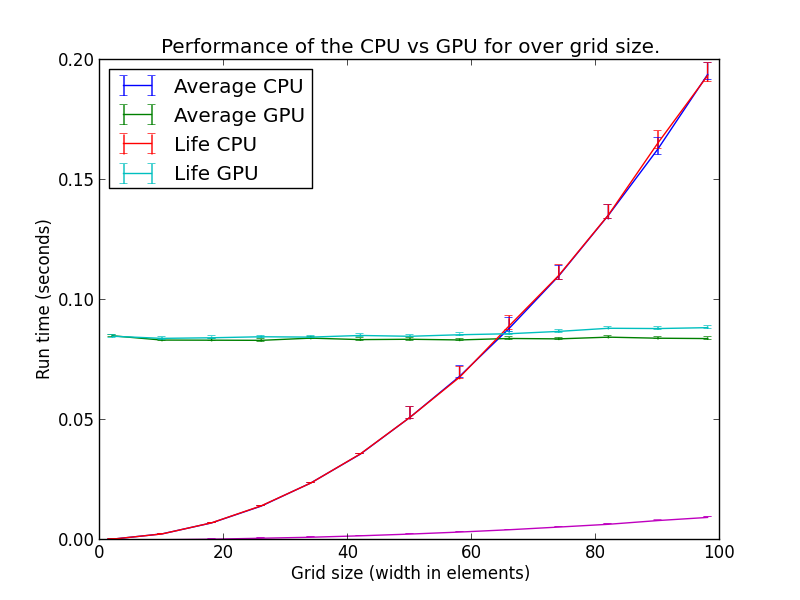
\includegraphics[width=\textwidth]{figs/run_performance.pdf}
  \caption{This plot shows the performance of the CPU versus the GPU
    implementations of the run primitive as it degrades with the grid size
    increasing. The grids are square in shape and the size given is for one of
    its dimensions. For comparison, both the average and game of life stencils
    are depicted. Also shown is the copy-on/off times for the GPU. Error bars
    are shown but most are vanishingly small.}
  \label{fig:runperf100}
\end{figure}

\begin{figure}[h]
  \includegraphics[width=\textwidth]{figs/run_performance2.pdf}
  \caption{This plot shows the performance of the GPU implementations of the run
    primitive as it degrades with a larger scale of grid size. Here we can see
    that both the Game of Life and average function diverge from the base
    measurement. Game of Life degrades the worst due to function calling
    overheads in its implementation. The CPU is not depicted as it grows too
    quickly, dwarfing the GPU measurements. }
  \label{fig:runperf1000}
\end{figure}

\begin{figure}[h]
  \includegraphics[width=\textwidth]{figs/run_performance3.pdf}
  \caption{Here we see the performance of the GPU on the same 0-1000 scale. Now
    the copy on/off time has been discounted by subtraction.}
  \label{fig:runperf1000dis}
\end{figure}

The results of the benchmarking showed that the GPU implementation outperforms
the CPU for grids of size greater than $30 \times 30$. This is in accordance
with the expected outcome, that the GPU is able to perform better modulo copy
on/off times.

On a scale of 0-100 (see \autoref{fig:runperf100}), the slowdown of the GPU
is barely visible above random variation. However, on a greater scale
(\autoref{fig:runperf1000}) it is clear that there is an increase in run
time.

The base measurement is the copy on/off time. We see that on the smaller scale
of analysis the base and actual stencils show little difference in performance
signifying that most of the time is spent in copying (between 20-50\% depending
on the stencil). On the greater scale we see how the stencil computations
actually diverge from the base as GPU computation time starts to become
significant. This can be seen more clearly in \autoref{fig:runperf1000dis}
where the copy on/off time has been discounted.

From the graphs we see that copy on/off time does not account for all the
overhead in the GPU computation. I hypothesise that this is due to a copy on/off
time for code as well as data (which was not accounted for in my
calculations). This is supported by the fact that the Game of Life has a greater
overhead at zero than the average function, because the implementation has
greater code size.

\subsubsection{Reduce}

\begin{figure}[h]
  \includegraphics[width=\textwidth]{figs/reduce_performance.pdf}
  \caption{This plot shows the performance of the CPU versus GPU versions of a
    reduction function. The reduction function given in this case in the sum
    function.}
  \label{fig:reduceperf}
\end{figure}

As we can see from \autoref{fig:reduceperf}, the performance of the reduce
primitive on the GPU also exceeds that of the CPU at $80\times80$ grid
size. This is a consequence of the fact that the reduction calculations are much
less intensive than those of the stencil function or the Game of Life.

\subsection{Deducing a model}

A future goal of this project might be to automatically decide when a certain
workload is best suited to the CPU or GPU. The experiments in this section have
already given us an insight into this: once grid size goes beyond a certain
size, the GPU should be used. We also saw that the complexity of the program
contributes to both the overhead and the scalability. However, at small values
of grid size the overhead of the GPU is most significant and so the degradation
can be ignored.

In order to deduce a model which could be used for switching between CPU and GPU
we must determine (a) an approximation function for the CPU's scalability, which
is mostly dependent on the grid size and (b) the overhead particular to our
program on the GPU, which depends on compiled code size as well as the grid
size. We will ignore (b) seeing as the evaluation was not sufficient to
determine this. (a) can be found by fitting a quadratic to the curve. This has
been done in \autoref{fig:fitting} and we can see that the quadratic
polynomial fits almost perfectly. The coefficients of this polynomial are given
by~\autoref{eq:quad}

\begin{equation} \label{eq:quad}
y = a x^2 + b x + c
\end{equation}
In this equation we can interpret $c$ as being the overhead for the CPU. The
coefficients are:
\begin{align*}
a & = & 3.23223432 \times 10^{-6}\\
b & = & -9.23861372 \times 10^{-6}\\
c & = & 1.56150424 \times 10^{-4}\\
\end{align*}

Knowing the particular overhead of our function, y, (as we have assumed) we are
now able to use \autoref{eq:quad} to calculate the grid size, $x$, for
which we should switch to using the GPU. We set $y$ to the run time of the GPU
operation (which we assumed is constant). Take $y=1.54 \times 10^{-3}$, as is
the case for the average stencil, then we get the resultant switching grid size
$x=22.17$ which agrees with the graph in \autoref{fig:runperf100}.

\begin{figure}[h]
  \includegraphics[width=\textwidth]{figs/run_performance_fit.pdf}
  \caption{Least square error fitting of a linear and quadratic curve to the
    performance data for the CPU implementation of the average function.}
  \label{fig:fitting}
\end{figure}

\section{Correctness}
\label{sec:correctness}

A central goal of the project was to produce a correct translation from Ypnos to
Accelerate. Already, by choosing a type safe language such as Haskell I vastly
reduced the number of run-time errors. To catch the rest I made use of
\emph{unit testing} and \emph{Test Driven Development} (TDD,
\autoref{sec:tdd}). Clearly, unit testing can only provide a partial assurance
of correctness and not a guarantee. However, I decided that a formal proof
(which could give these guarantees) was beyond the scope of this project. In
writing these tests I have assumed that the original CPU implementation was
correct and could be compared against as a gold standard\footnote{However, in
  running my tests I uncovered a bug in the implementation of boundaries which
  had to be fixed before this assumption could hold.}.

The testing framework used works slightly differently to other unit testing
frameworks. In a standard framework the user provides test cases which
incorporate both the test data (sometimes generated) and assertions. In
Haskell's \emph{QuickCheck} we only provide axioms about our functions and let
the framework provide the data based on the type.

Typically, QuickCheck will generate hundreds of test samples to verify a
particular axiom. This provides a better assurance than ordinary unit
testing as, via the random process, QuickCheck often comes up with corner
cases the programmer may not have devised themselves.

The following sections of my project required unit testing:

\begin{itemize}
\item The centring algorithm for grid patterns, as this contains a large part of
  the translations complexity.
\item The \texttt{funGPU} quasiquoter.
\item The \texttt{run} primitive.
\item The \texttt{reduce} primitive.
\end{itemize}

The approach taken to testing the grid patterns was to ensure that the
transformation:

\begin{itemize}
\item
  Starts with a grid that has certain properties (a precondition):
  regular size, positive size, has a cursor.
\item
  Maintains the regularity of size: the length of each row is the same.
\item
  Centres the cursor, given the original grid had a cursor.
\item
  Both roffset and coffset are always positive on such a grid (see
  \autoref{sec:centring} for an explanation of these two values).
\end{itemize}

The assumption was that grid patterns given to the transformation procedures
would be correct to begin with. As such, to improve the amount of test data
generated, I enforced these properties at the generation level. This is safe as
the grid patterns are generated through the CPU translation which I was assuming
to be correct.

To test the primitives I used a standard testing approach of comparing against a
reference implementation. For the \texttt{reduce} primitive I compare against
Haskell's built-in reduce function as I can safely assume this to be
correct. For the \texttt{run} primitive I originally intended to test against
the Ypnos CPU implementation.

The run primitive is tested by running the average function on a randomly
generated grid. The grid is passed to the GPU and CPU implementations of
\texttt{avg}. The resulting grid is then compared between the two and any
difference counts as a failure.

The same procedure is used for the reduce primitive. We use a one-dimensional
grid for this case as the built-in Haskell function we are comparing against is
one-dimensional. The resulting reduced values are compared and a failure is
registered if they should differ.

\section{Usability}

While not mentioned in my original proposal, the usability to the programmer is
another non-functional requirement. This project lacked time for a full
usability study. Instead, evaluated the usability using the method of
\emph{Cognitive Dimensions}~\cite{green96}, to compare the various approaches
already discussed.

Cognitive Dimensions of notations (CD) provide a light-weight vocabulary for
discussing various factors of programming language design. As Ypnos is
essentially a programming language (albeit, one embedded in Haskell) it makes
sense to use this technique. It works by specifying a number of properties of a
notation (\emph{dimensions}, a complete list can be found in
Green\cite{green96}) which must, in general, be traded off against one
another. For this reason it is important to understand the representative tasks
and the user that will be performing them. Then design decisions in the language
can be compared and evaluated using the dimensions relative to the tasks.

\subsection{System = Language + Environment}

It is important to note that CD relates to a whole system, not just the
language. We define the system to be the combination of programming language and
the programming environments. For example, programming over the phone versus
programming in a visual editor. For the purposes of discussing only the language
changes that I have introduced I will fix the environment and assume that it has
the following features:

\begin{itemize}
\item
  Screen-based text editor (e.g.~Vim, Emacs or TextMate)
\item
  Search and replace functionality (including regular expressions)
\end{itemize}

\subsection{Methodology}

I used the following procedure in evaluating the changes to Ypnos using
CD:

\begin{itemize}
\item
  Identify the relevant users of my system and sketch out a basic user
  profile.
\item
  Select the relevant task of these users on the part of the language I
  implemented.
\item
  Highlight which cognitive dimensions are most important to the selected tasks.
\item
  Show a comparison of the various approaches to this implementation.
\item
  Conclude which approach was taken and why.
\end{itemize}

\subsection{User profiles}

I have decided that given the applications to scientific computing and graphics,
the two main types of users would be scientists simulating physical systems and
graphics programmers developing graphics algorithms. I have included two user
stories for our two representative users:

\begin{shadequote}
  Kiaran is a physical scientist who is writing a simulation of a fluid dynamics
  system. He has a little Haskell experience already but has mostly used other
  languages such as Matlab and Fortran. He chose Ypnos/Haskell because he knew
  it would allow him to easily switch between a CPU implementation on his
  machine and a GPU implementation on the simulation machine he is using.
\end{shadequote}

\begin{shadequote}
  Noemi is writing a graphics transformation for a photo editing package. The
  photos her users edit are typically very large but she still would like to
  provide real-time performance with her algorithms. Noemi has a GPU in her
  computer, so she will be writing for this to ensure that her performance is
  good. However, she also wants her system to work on machines that do not have
  a compatible GPU. She already has experience in Haskell and is familiar with
  more complex features and extensions such as type and data families. She has
  picked Ypnos/Haskell because of its syntax and multiple backends.
\end{shadequote}

We can see that there are many tasks that these users would want to
perform with our system: coding up a filter into a stencil (Noemi),
writing a complex reduction to determine the state of the system
(Kiaran), debugging to find out why they get the wrong values (both).
However, I will be ignoring all tasks that involve parts of the system
which I did not implement. This leaves us with one central task for the
two use cases: converting between GPU and CPU.

The cognitive dimensions relevant to this task are:

\begin{tabular}{p{0.35\textwidth} p{0.6\textwidth}}
  Low repetition viscosity & to allow the programmer to easily change the
  implementation without changing too many points in code.
  \\
  Little to no imposed lookahead & allowing the programmer to use one
  implementation without having to think about later switching.
  \\
  Consistency & the programs syntax or usage does not change from CPU to
  GPU, e.g. changing only constructor names.
  \\
  Terseness & the syntax to specify the implementation does not get in the
  way of coding the stencils.
  \\
  Closeness of mapping & the model presented to the programmer through the API
  should map well to their mental model for these types of operation,
  e.g. comonadic operations.
  \\
\end{tabular}

The various approaches to provide an API to the programmer were discussed in the
\autoref{chap:impl}. They essentially boiled down to the following three
approaches: choosing the different implementation based on importing (also
called the non-unifying approach, see \autoref{sec:non-unify-appr}), using
type classes with associated data families (\autoref{sec:assoc-data-fam})
and using type classes with associated type families
(\autoref{sec:assoctypefam} and \autoref{sec:final}). For the sake of
comparison I will also include the approach of the programmer re-coding their
implementation in Accelerate for the GPU.

The results of the evaluation are briefly summarised in
\autoref{tbl:cogcompbrief}, for a full discussion see \autoref{tbl:cogcomp}
in the Appendix. An informal usability analysis such as this one was performed
at the end of each iterative development phase in order to inform the next
prototype.

\begin{longtable}{r | l l l l}
\hline

CD & Accelerate & Non-unifying & Data families & Type families

\\ \hline

Repetition viscosity & \textbf{Worst} & & & \textbf{Best}
\\

Imposed lookahead & \textbf{Worst} & \textbf{Best} & \textbf{Best} &
\textbf{Best}
\\

Consistency & \textbf{Worst} & & & \textbf{Best}
\\

Terseness & \textbf{Worst} & & & \textbf{Best}
\\

Hidden dependencies & \textbf{Best} & \textbf{Worst} & \textbf{Best} &
\textbf{Worst}
\\

Abstraction gradient & \textbf{Best} & & &
\\

Closeness of mapping & \textbf{Best} & \textbf{Worst} & \textbf{Worst} &
\textbf{Worst}
\\
\hline

\caption{A short comparison of the different APIs using cognitive
  dimensions. \label{tbl:cogcompbrief}}
\end{longtable}

\subsection{Discussion of Usability}

As we now can see, the best approach for our users is that of associated type
families with the data constructor for the stencil function. This approach is
best in the viscosity, imposed lookahead, consistency and terseness
dimensions. However, for this it has compromised in hidden dependencies,
abstraction and closeness of mapping.

The \emph{hidden dependency} problems are mitigated by the Haskell compiler
which warns and throws errors when there is a conflict in these dependencies,
e.g. if the user uses different \texttt{Sten} type constructors on the same grid
(see \autoref{lst:stendatafam}). While a little increase in hidden
dependencies is necessary to reduce viscosity, there could be room for
improvement here by making the types more consistent. This would help us remove
the dependencies due to the changing types and constraints.

Given that our example users are fairly advanced, the increase in
\emph{abstraction} should not be a problem, however, we should be aware of this
extra difficulty to learning the language. Advanced features such as type
families are hidden from the users in most cases, so Kiaran should not have a
problem.

The \emph{closeness of mapping} is an issue that is not inherent in the
implementation, but rather an artifact of it. With more time on this
project I would try to re-introduce the comonadic types to the type
family approach. This could require using a lower level implementation
rather than using Accelerate. For this reason getting a closer mapping
was beyond the scope of this project.

\section{Summary}

In this chapter we saw how the performance of my GPU implementation surpasses
that of the CPU for larger grid sizes. This holds for both the run and reduce
primitives. I demonstrated the testing approach taken and discussed how this can
provide some assurance as to the correctness of the translation. Finally, I
conducted usability evaluation using the method of cognitive dimensions.

In summary, this chapter demonstrated all the requirements of the project
(\autoref{sec:reqanal} and original proposal in \autoref{chap:prop}) have been
fulfilled:
\begin{enumerate}
\item Compilation of Ypnos code and implementation of the run primitive on the
  GPU.
\item Implementation of the reduce primitive on the GPU.
\item Better scaling than the current single threaded implementation when
  accounting for copy-on/off times.
\item The translation correctly preserves the semantics of Ypnos.
\end{enumerate}

Furthermore, I have demonstrated the usability of my API, a goal which was not
originally stated.

\chapter{Conclusion}

During this project I have learnt a large number of new and complicated
technologies from a field of computer science previously unknown to me. Having
only experienced the ML functional programming from Part Ia, diving into
Haskell's intricate type system has been an enlightening experience which has
taught me much about my personal software engineering approach and the type
systems of other languages.

\section{Accomplishments}

In this project I have managed to accomplish all the goals laid out by the
original proposal: a correct translation and run primitives which out-perform
their CPU counterparts. Furthermore, I conducted usability evaluation which was
not originally conceived as a requirement.

Aside from the mechanical goals of the project I have also deepened my own
knowledge of computer science and software engineering. I can now add Haskell to
the list of languages I am intimately familiar with. My experience with Haskell
has given me a better understanding of the type theoretic decisions that
underpin other more common languages (such as the various types of polymorphism
used in OOP). Furthermore, my software engineering approaches have been improved
by often needing to re-factor code and design complex systems such as the
centring algorithm.

I consider the project a success in that it both accomplished the requirements
(see \autoref{chap:evaluation}), providing a step forward for the Ypnos
programming language, and helped me learn much about Haskell and GPU
computation.

\section{Lessons Learnt}

In completing this project I have learnt the importance of having a strong plan
to stick to. I realised as I went further into this project that I had not
allocated enough time to researching and learning a new programming
ecosystem. Particularly, I had severely underestimated the time it would take to
get familiar with the complex type theory underlying the Haskell compiler.

Furthermore, if I were to repeat the project I would set out better procedures
for making notes and documenting the project as it progressed. The time required
to compile all the information for the dissertation and understand the different
approaches taken in the implementation was significantly more than I had
previously anticipated. In future work I will endeavour to keep a more complete
diary with frequent reviews of all the work accomplished so far and how it all
fits together.

\section{Future Work}

While all the goals of this project have been achieved, the path of accelerating
Ypnos on the GPU is by no means complete. A number of extensions from the
original proposal still have not been attempted, which include:

\begin{itemize}
\item The \texttt{iterate} primitive which would allow more efficient execution
  of pipelined operations.
\item The \texttt{zip} primitive which would allow implementation of more
  complicated algorithms which require multiple parameters. This would allow
  programs such as \emph{Canny edge detection} to be implemented.
\end{itemize}

Further to the original extensions, during the course of the project more
possible avenues for exploration were discovered. Further exploration may be
possible in:

\begin{itemize}
\item
  Attempting to expose the comonadic nature of operations in the type given to
  the programmer.
\item
  Deducing a full model for the GPU computation overhead.
\item
  Automatic selection of the backend dependent on static program analysis.
\end{itemize}

\printbibliography[heading=bibintoc]

\appendix

\chapter{Original Proposal}
\label{chap:prop}


% Draft #2


% Main document

\bibliographystyle{plain}

\section*{Introduction, The Problem To Be Addressed}

In recent years, Moore's law has begun to plateau. As a result the hardware 
industry has increasingly been turning to MIMD and SIMD architectures as a 
solution.  Some of the highest performing SIMD implementations today are 
provided by GPUs and can be harnessed via GPGPU languages such as CUDA and 
OpenCL.  However, taking advantage of GPGPU is hard as it requires knowledge of 
the low-level concepts of these languages. It is also not portable between 
different hardware and methods of concurrency.

Structured grids are a common computational pattern for scientific parallel 
computation. They allow us to specify \emph{stencils} or \emph{kernels} which 
are local computations that compute a new value from neighboring cells.  
Stencils are promoted to operations over the whole array by application to 
every index.  Many algorithms can be described in this way including the 
Gaussian blur filter, edge detection as well as scientific applications such as 
fluid dynamics. It is also possible to highly parallelize this computation by 
splitting the grid into smaller chunks and running the stencil on each 
separately.

Ypnos \cite{ypnos} is an Embedded Domain Specific Language in the Haskell 
programming language that is capable of describing and running these kernels 
over a grid.  It defines a syntax and various primitives for the structured 
grid computation.  

A kernel is described using a modified Haskell function syntax. The following 
is a kernel used to compute the Gaussian of a grid. The arguments are written 
as a grid and the central point is annotated with \verb|@|. It also denotes the 
location where the kernels return value is written in the new grid.

\begin{verbatim}
ave2D :: Grid (X * Y) Double -> Double
ave2D (X * Y): | _  t _ | = (t+l+c+r+b)/5.0
               | l @c r |
               | _  b _ |
\end{verbatim}

The \emph{run} primitive is used to lift the stencil to a grid operation and 
\emph{iterate} primitive simply recursively applies run. The \emph{reduce} 
primitive allows us to summarise the data so that we can calculate means, sums, 
minimums or maximums. This result is often used as a stopping condition for 
iteration.

The \emph{zip} and \emph{unzip} primitives allow us to pair and unpair the 
values of two grids respectively. This is useful when dealing with multiple 
inter-related quantities as is the case in a physical system with force, 
acceleration and velocity.

Due to the declarative syntax and its purity the order of application of the 
stencils is not important. The author of an Ypnos program does not need to 
worry about the method of concurrency underpinning their program. This allows 
the implementers of Ypnos to use whichever method is most appropriate for the 
given work load and computer. As many computers these days are equipped with 
very advanced GPUs capable of general purpose computation, the Ypnos language 
should be able to use these to accelerate its calculations.

\section*{Starting Point}

\begin{itemize}

\item I have had experience of functional programming from the course as well 
as having completed some Haskell tutorials. 

\item I have experience of building a compiler from Part IB supervision work.

\item During the course of an 11 week internship I learnt to plan, implement, 
document and test my own project.

\item I have already read the Ypnos paper and am familiar with the constructs 
of the language as well its primitives.

\item At present Ypnos has been partially implemented in a single threaded 
fashion on the CPU. The proof-of-concept is only partially implemented. This 
implementation can be taken as both the starting point and the benchmark for 
the new implementation.

\item A Haskell ESDL already exists for compiling array computations to CUDA 
code. The library, ``accelerate'' \cite{accel}, takes an AST and produces code
to run on the GPU.  I will use this library as a back-end to avoid writing a 
compiler to CUDA code directly.

\end{itemize}

\section*{Resources Required}

\begin{itemize} 

\item For this project I shall require my own laptop computer that runs Arch 
Linux for the bulk of development work. 

\item Backup will be to github, the SRCF and/or the MCS. Should my computer 
fail I will be able to use the MCS computers for the project.

\item I require an Nvidia GPU in order to test the code produced. This will be 
provided by Dominic Orchard and I will have access to the machine via SSH for 
testing purposes.

\end{itemize}

\section*{Work to be done}

The project breaks down into the following sub-projects:

\begin{enumerate}

\item Write unit tests that can be used to check the correctness of my 
implementation. The tests will cover micro aspects of the programming language 
such as: constants, unary application, binary application, indexing, 
conditionals, local let-binding, etc.

\item The implementation of the main compilation. This involves writing a 
compilation pass that can take the Ypnos AST and produce a correspondent 
``accelerate'' AST.

\item The implementation of the basic \emph{run} and \emph{reduce} primitives 
as well as any combinators for constructing and deconstructing arrays from raw 
data. The combinators may be written in the ``accelerate'' language directly.

\item The testing of the implementation to check that it works correctly and is 
faster than the original modulo data copying. This will need a test bench to be 
constructed that includes various well know stencil computations. The test 
bench will include the following programs as a minimum: the Game of Life, 
Gaussian blur, Canny edge detection, and (if zip/unzip are implemented) the 
difference of Gaussians.

\end{enumerate}

\section*{Success Criterion for the Main Result}

The project will be a success if:

\begin{enumerate}

\item It can compile Ypnos code and implements the \emph{run} primitive on the 
GPU.

\item It implements the \emph{reduce} primitive on the GPU.

\item It scales better than the current single threaded implementation on large 
work loads. That is to say that when the domain size is increased, the 
difference in computation time increases too. However, this must take into 
account the time required to copy data on and off the GPU.

\item It does all of the above correctly and passes the initial unit tests.

\end{enumerate}

\section*{Possible Extensions}

If the main aim for this project is achieved then I shall try to implement 
further primitives of the Ypnos language. The programmer will then be able to 
take advantage of the speed gains of the GPU pipeline. I will attempt them in 
this order:

\begin{enumerate}

\item The ``iterate'' primitive. This will eliminate the need to copy data 
between the CPU and GPU at each step.

\item The ``zip'' primitive.

\end{enumerate}

I may also attempt to enhance the compiler to decide at compile-time whether to 
use the GPU or CPU dependant on the size of computation required.

\section*{Timetable: Workplan and Milestones to be achieved.}

Planned starting date is 19/10/2011 when the proposal is accepted.

\subsection*{Michaelmas weeks 2-4} Learn to write and read Haskell code. Write 
some programs in Ypnos. Try to understand the existing code base. Start writing 
a unit testing suite.

\subsection*{Michaelmas weeks 5-6} Finish writing the unit testing suite by 
including Gaussian blur and Game of Life programs. Get familiar with the 
``accelerate'' ESDL by reading the paper and writing some toy programs. 

\subsection*{Michaelmas weeks 7-8} Start implementation of the compiler from 
the Ypnos AST to the ``accelerate'' AST. Most basic operations should translate 
correctly by this point.

\subsection*{Michaelmas vacation} Finish the compiler and begin work on 
implementing the run and reduce primitives.

\subsection*{Lent weeks 0-2} Finish the primitives if necessary. Write the 
progress report. Start work on the basic test bench.

\subsection*{Lent weeks 3-5} Finalise the main test bench and run experiments.  
Analyse the performance and scalability of the approach. Make improvements to 
the code as necessary to achieve the main aim of the project. 

\subsection*{Lent weeks 6-8} If there is time then the main extensions may be 
implemented at this point.

\subsection*{Easter vacation} Write the main chapters of the dissertation.

\subsection*{Easter term 0-2} Elaborate on the existing tests bench and run 
final experiments. Complete the dissertation.

\subsection*{Easter term 3} Proof reading and then an early submission.  

\bibliography{refs}


\chapter{Full Cognitive Dimension Analysis}
\label{chap:cogdim}

\newcommand{\sideways}[1]{
  \parbox[t]{2mm}{{\rotatebox[origin=r]{90}{#1}}}}
\newlength{\fstcollen}
\newlength{\sndcollen}
\setlength{\fstcollen}{0.5cm}
\setlength{\sndcollen}{(\textwidth-\fstcollen-2cm)/4}
\begin{longtable}{r | p{\sndcollen} p{\sndcollen} p{\sndcollen} p{\sndcollen}}
\hline\noalign{\medskip}

\sideways{CD}
 &
Accelerate
 &
Non-unifying
 &
Data families
 &
Type families (only stencil data type)

\\\noalign{\medskip}
\hline\noalign{\medskip}

\sideways{Repetition viscosity}
 &
\textbf{Worst}

Clearly here we have a very high viscosity: each function must be re-written in terms of new syntax and run in different ways.
 &
We have improved the viscosity significantly. The user must only
implement their stencils in one language but they must still change all
the imports and correct type errors.
 &
Data families worsen the viscosity over the import method as we must now
change all the data constructors as opposed to the imports. In real code
there will be more of these than import locations.
 &
\textbf{Best}

Here we have the least repetition viscosity of all the approaches. We
now only need to change the quasi quoter to change the whole
implementation.

\\\noalign{\medskip}

\sideways{Imposed lookahead}
 &
\textbf{Worst}

The user must know ahead of time that they will be writing in two
languages to be sure to minimize duplication of code and structure their
program correctly.
 &
\textbf{Best}

There is practially no imposed lookahead as we can simply swap out the
implementation by importing from different places.
 &
\textbf{Best}

We do not have imposed lookahead as we can easily swap the constructors.
 &
\textbf{Best}

There is little imposed lookahead in theory, though some operations are
currently not supported in the GPU implementation. (TODO: link to more)
Some types may not be supported easily in both implementations so this
should be considered too.

\\\noalign{\medskip}

\sideways{Consistency}
 &
\textbf{Worst}

The syntaxes are different and so are fairly inconsistent. There are,
however, some similarities between the two in their stencil
representation.
 &
Consistency is improved as the syntax is now uniform but types are not
uniform.
 &
The syntax and usage is the same except for changing the constructors
which is inconsistent.
 &
\textbf{Best}

We have eliminated the inconsistency in usage of the data families. Now
the approach is almost entirely consistent except for the types.

\\\noalign{\medskip}

\sideways{Terseness}
 &
\textbf{Worst}

A lot of code is written by the user to cope with the two different
implementations.
 &
Changing requires a fair bit of code to be changed as we may be
importing many different things from the Ypnos libraries and all these
things must be changed.
 &
We require a lot of code to express the swap from CPU to GPU.
 &
\textbf{Best}

The syntax for switching is minimally terse.

\\\noalign{\medskip}

\sideways{Hidden dependencies}
 &
\textbf{Best}

No hidden dependencies. It is very clear and explicit what is going on.
 &
\textbf{Worst}

Many hidden dependencies are introduced as the types of the different
imported functions do not necessarily match. This can cause failures in
many different places on changing the import.
 &
\textbf{Best}

Here the dependencies introduced in the type system by the import
approach have been made explicit by data constructors.
 &
\textbf{Worst}

More hidden dependencies are introduced. Types change without the users knowing
due to different type and constraint families. This might affect some programs.

\\\noalign{\medskip}

\sideways{Abstraction gradient}
 &
\textbf{Best}

The abstraction is at its most basic level -- choosing between Ypnos or
Accelerate. The user must get to grips with these abstractions as a
minimum.
 &
The abstraction level is fairly low as it uses only simple Haskell
constructs.
 &
The user must now be familiar with the idea of an associated data family
and GADT which are quite advanced Haskell type features.
 &

The abstraction here is perhaps highest of all as it uses the most
advanced type features.

\\\noalign{\medskip}

\sideways{Closeness of mapping}
 &
\textbf{Best}

This way we preserve the comonadic nature of the operations in the type
so that it is obvious to the user what is going on.
 &
\textbf{Worst}

The comonadicity is lost due to having to change the types to suit the
accelerate implementation.
 &
\textbf{Worst}

The comonadicity is lost also.
 &
\textbf{Worst}

The comonadicity is lost.

\\\noalign{\medskip}
\hline
\noalign{\medskip}
\caption{Comparison of the different API using cognitive dimensions. \label{tbl:cogcomp}}
\end{longtable}


\end{document}
